\documentclass[10pt, a4paper]{article}
\usepackage[slovene]{babel}
\usepackage[T1]{fontenc}
\usepackage[utf8]{inputenc}
\usepackage{lmodern}
\usepackage{amsmath}
\usepackage{amsthm}
\usepackage{amssymb}
\usepackage{parskip}
\usepackage{pgfplots}
\pgfplotsset{compat=1.16}
\usepgfplotslibrary{colormaps,fillbetween}
\usepackage{comment}
\usepackage{graphicx}
\usepackage{booktabs}
\usepackage{array}
\usepackage{subfig}
\usepackage{asymptote}
%\usepackage{mdframed}
%\usepackage{thmbox}

%%%%%%%%%%%%%%%%%%%%%%%%%%%%%%%%%%%%%%%%%%%%%%%%%%%%%%%%%%%%%%%%%%%%%%

\usepackage[top=105pt, bottom=75pt, left=75pt, right=75pt]{geometry}
\setlength{\headsep}{15pt}
\setlength{\footskip}{45pt}

\usepackage{xcolor}
\usepackage{lipsum}
%\usepackage{unicode-math}

\usepackage{ifthen}
\usepackage{tikz}
\usepackage{amsfonts}
\usetikzlibrary{calc}
\usetikzlibrary{cd}
\usetikzlibrary{babel}
\usetikzlibrary{arrows,arrows.meta,bending,decorations.markings,intersections}
\definecolor{fcolor}{RGB}{0,255,255}

\tikzset{% https://tex.stackexchange.com/a/430239
    arc arrow/.style args={%
    to pos #1 with length #2}{
    decoration={
        markings,
         mark=at position 0 with {\pgfextra{%
         \pgfmathsetmacro{\tmpArrowTime}{#2/(\pgfdecoratedpathlength)}
         \xdef\tmpArrowTime{\tmpArrowTime}}},
        mark=at position {#1-\tmpArrowTime} with {\coordinate(@1);},
        mark=at position {#1-2*\tmpArrowTime/3} with {\coordinate(@2);},
        mark=at position {#1-\tmpArrowTime/3} with {\coordinate(@3);},
        mark=at position {#1} with {\coordinate(@4);
        \draw[-{Stealth[length=#2,bend]}]       
        (@1) .. controls (@2) and (@3) .. (@4);},
        },
     postaction=decorate,
     },arr/.style={arc arrow=to pos #1 with length 2.3mm}
}
%%%%%%%%%%%%%%%%%%%%%%%%%%%%%%%%%%%%%%%%%%%%%%%%%%%%%%%%%%%%%
\usepackage{tcolorbox}
\tcbuselibrary{skins, breakable}


%%%%%%%%%%%%%%%%%%%%%%%%%%%%%%
%%% with separate title
\xdefinecolor{thmTopColor}{RGB}{102, 102, 238}
\xdefinecolor{thmBackColor}{RGB}{245, 245, 255}

%%%%%%%%%%%%%%%%%%%%%%%%%%%%%%%%%%%%%%%%%%%%%%%%%%%%%%%%%%%%%%%%%%%%%%%%

\graphicspath{ {./images/} }

\newtheorem{izr}{Izrek}[section]

\newenvironment{thmbox}[1]{%
  \tcolorbox[%
  empty,
  parbox=false,
  noparskip,
  enhanced,
  breakable,
  sharp corners,
  boxrule=-1pt,
  left=2ex,
  right=0ex,
  top=0ex,
  boxsep=1ex,
  before skip=2.5ex plus 2pt,
  after skip=2.5ex plus 2pt,
  colback=thmBackColor,
  colframe=white,
  coltitle=black,
  colbacktitle=thmBackColor,
  fonttitle=\bfseries,
  title=#1,
  titlerule=1pt,
  titlerule style=thmTopColor,
  overlay unbroken and last={%
    \draw[color=thmTopColor, line width=1.25pt]
    ($(frame.north west)+(.5em, -4.1ex)$)
    -- ($(frame.south west)+(.5em, 1ex)$) -- ++(2em, 0);
  }]
}{\endtcolorbox}

\newenvironment{izrek}[1][]{% before
  \refstepcounter{izr}%
  \ifthenelse{\equal{#1}{}}{%
    \begin{thmbox}{Izrek \theizr.}\itshape\hspace{-.75ex}%
  }{%
    \begin{thmbox}{Izrek \theizr%
        \hspace{.75ex}(\textnormal{#1}).}\itshape\hspace{-.75ex}
    }}
  {\end{thmbox}
}

{\theoremstyle{plain}
\newtheorem{posledica}[izr]{Posledica}
\newtheorem{trditev}[izr]{Trditev}

}

{\theoremstyle{definition}
\newtheorem{defi}{Definicija}[section]
\newtheorem{aksiom}{Aksiom}[section]
}

\newenvironment{noticeB}{%
  \tcolorbox[%
  notitle,
  empty,
  enhanced,  % delete the edge of the bottom page for a broken box
  breakable,
  coltext=black,
  colback=white, 
  fontupper=\rmfamily,
  parbox=false,
  noparskip,
  sharp corners,
  boxrule=-1pt,  % width of the box' edges
  frame hidden,
  left=7pt,  % inner space from text to the left edge
  right=7pt,
  top=5pt,
  bottom=5pt,
  % boxsep=0pt,
  before skip=2.5ex plus 2pt,
  after skip=2.5ex plus 2pt,
  borderline west = {1.5pt}{-0.1pt}{blue!30!black}, % second argument = offset
  overlay unbroken and last={%
    \draw[color=black, line width=1.25pt]
    ($(frame.south west)+(1.pt, -0.1pt)$) -- ++(2em, 0);
  }
  ]}
{\endtcolorbox}

\newenvironment{definicija}{\begin{defi}\begin{noticeB}}{%
    \end{noticeB}\end{defi}}

{\theoremstyle{remark}
\newtheorem*{opomba}{Opomba}
}

\newtheorem{zgled}{Zgled}[section]
\tcolorboxenvironment{zgled}{%
  enhanced jigsaw,
  boxrule=-1pt,
  colframe=gray!15,
  %borderline west={2pt}{0pt}{black},  % second argument is the offset
  interior hidden,
  sharp corners,
  breakable,
  before skip=2.5ex plus 2pt,
  after skip=2.5ex plus 2pt
}

%%%%%%%%%%%%%%%%%%%%%%%%%%%%%%%%%%%%%%%%%%%%%%%%%%%%%%%%%%%%%%%%%%%%%%%%
\newtheorem{lema}[izr]{Lema}
\tcolorboxenvironment{lema}{%
  enhanced jigsaw,
  boxrule=-1pt,
  sharp corners,
  colframe=white,
  borderline west={2pt}{0pt}{orange},  % second argument is the offset
  interior hidden,
  breakable,
  before skip=2.5ex plus 2pt,
  after skip=2.5ex plus 2pt
}

%%%%%%%%%%%%%%%%%%%%%%%%%%%%%%%%%%%%%%%%%%%%%%%%%%%%%%%%%%%%%%%%%%
\newenvironment{noticeC}{%
  \tcolorbox[%
  notitle,
  empty,
  enhanced,  % delete the edge of the bottom page for a broken box
  breakable,
  coltext=black, 
  fontupper=\rmfamily,
  parbox=false,
  noparskip,
  sharp corners,
  boxrule=-1pt,  % width of the box' edges
  frame hidden,
  left=7pt,  % inner space from text to the left edge
  right=7pt,
  top=5pt,
  bottom=5pt,
  % boxsep=0pt,
  before skip=2.5ex plus 2pt,
  after skip=2.5ex plus 2pt,
  %borderline west = {1.5pt}{-0.1pt}{gray}, % second argument = offset
  overlay unbroken and last={%
    %\draw[color=gray, line width=1.25pt]
    %($(frame.west)$);
    %\draw[color=gray, line width=1.25pt]
    %($(frame.east)$);
  },
  ]}
{\endtcolorbox}

\newenvironment{dokaz}%
  {\begin{noticeC}\begin{proof}}%
  {\end{proof}\end{noticeC}}

%%%%%%%%%%%%%%%%%%%%%%%%%%%%%%%%%%%%%%%%%%%%%%%%%%%%%%%%%%%%%%%%%%%%

\makeatletter
\newlength\xvec@height%
\newlength\xvec@depth%
\newlength\xvec@width%
\newcommand{\xvec}[2][]{%
  \ifmmode%
    \settoheight{\xvec@height}{$#2$}%
    \settodepth{\xvec@depth}{$#2$}%
    \settowidth{\xvec@width}{$#2$}%
  \else%
    \settoheight{\xvec@height}{#2}%
    \settodepth{\xvec@depth}{#2}%
    \settowidth{\xvec@width}{#2}%
  \fi%
  \def\xvec@arg{#1}%
  \def\xvec@dd{:}%
  \def\xvec@d{.}%
  \raisebox{.2ex}{\raisebox{\xvec@height}{\rlap{%
    \kern.05em%  (Because left edge of drawing is at .05em)
    \begin{tikzpicture}[scale=1]
    \pgfsetroundcap
    \draw (.05em,0)--(\xvec@width-.05em,0);
    \draw (\xvec@width-.05em,0)--(\xvec@width-.15em, .075em);
    \draw (\xvec@width-.05em,0)--(\xvec@width-.15em,-.075em);
    \ifx\xvec@arg\xvec@d%
      \fill(\xvec@width*.45,.5ex) circle (.5pt);%
    \else\ifx\xvec@arg\xvec@dd%
      \fill(\xvec@width*.30,.5ex) circle (.5pt);%
      \fill(\xvec@width*.65,.5ex) circle (.5pt);%
    \fi\fi%
    \end{tikzpicture}%
  }}}%
  #2%
}
\makeatother

% --- Override \vec with an invocation of \xvec.
\let\stdvec\vec
\renewcommand{\vec}[1]{\xvec[]{#1}}
% --- Define \dvec and \ddvec for dotted and double-dotted vectors.
\newcommand{\dvec}[1]{\xvec[.]{#1}}
\newcommand{\ddvec}[1]{\xvec[:]{#1}}
\newcommand{\stcomp}[1]{{#1}^{\mathsf{c}}}

%%%%%%%%%%%%%%%%%%%%%%%%%%%%%%%%%%%%%%%%%%%%%%%%%%%%%%%%%%%%%%%%%%%%

\newcommand{\N}{\mathbb {N}}
\newcommand{\Z}{\mathbb {Z}}
\newcommand{\Q}{\mathbb {Q}}
\newcommand{\R}{\mathbb {R}}
\newcommand{\C}{\mathbb {C}}
\newcommand{\zap}[1]{(#1_n)_{n=1} ^{\infty}}
\newcommand{\podzap}[1]{(#1_{n_j})_{n=1 ^{\infty}}}
\newcommand{\limzap}[1]{\lim_{n \to \infty} {#1}}
\newcommand{\ve}[1]{\overrightarrow{#1}}
\newcommand{\vectors}[2]{\vec{{#1}_1},\vec{{#1}_2}, \dots \vec{{#1}_{#2}}}
\newcommand{\scalars}[2]{{#1}_1, {#1}_2, \dots, {#1}_{#2}}
\newcommand{\im}{\mathrm{Im}\,}
\newcommand{\re}{\mathrm{Re}\,}
\newcommand{\rang}{\mathrm{\text{rang}}\,}
\newcommand{\isom}{\stackrel{\sim}{=}}
\newcommand{\quot}[2]{{\raisebox{.2em}{$#1$}\left/\raisebox{-.2em}{$#2$}\right.}}
\newcommand{\sprod}[2]{\left\langle {#1},{#2} \right\rangle}
\newcommand{\cl}{\mathrm{Cl}}
\newcommand{\inte}{\mathrm{Int}}
\newcommand{\fr}{\mathrm{Fr}}
\newcommand{\F}{\mathcal{F}}
\newcommand{\grad}{\mathrm{grad}\, }
\newcommand{\divg}{\mathrm{div}\, }
\newcommand{\rot}{\mathrm{rot}\, }
\newcommand{\Mod}[1]{\ (\mathrm{mod}\ #1)}
\newcommand{\res}[2]{\mathrm{Res}\, \left(#1, #2\right)}
\DeclareMathOperator{\di}{d\!}

\newcolumntype{C}[1]{>{\centering\let\newline\\\arraybackslash\hspace\hspace{0pt}}m{#1}}

\setlength{\parskip}{1em}


\begin{document}

\title{ANALIZA 2b - ZAPISKI}
\author{Gal Anton Gorše}
\date{}
\maketitle

\section{MNOGOTEROSTI}

\subsection{Podmnogoterosti v $\R^n$}

Posplošiti skušamo pojme krivulj in ploskev. Če imamo diferenciabilno preslikavo
$F : D \subseteq \R^n \to \R^m$ v točki $a \in D$, pravimo, da je $F$ v $a$ ranga $r$,
če ima matrika $(DF) (a)$ rang $r$. Prav tako lahko rečemo, da je $F$ ranga $r$, če to velja za $\forall a \in D$.
$F$ ima v $a \in D$ maksimalen rang, če je $\rang (DF) (a) = \min \{m, n\}$.
Če je $F \in C^1$ in $\rang (DF) (a) = \min\{m, n\}$, je $\rang (DF) (x) = \min \{m, n\}$, tudi v okolici $a$.

\begin{definicija}
    Neprazna množica $M \subseteq \R^{n + m}$ je $n$-dimenzionalna, gladka (vsaj $C^1$)
    podmnogoterost (kodimenzije $m$), če za vsako točko $a \in M$ obstaja okolica $U$
    točke $a$ v $\R^{n + m}$ in $C^1$ definicijske funkcije $F_1, \dots, F_{m}: U \to \R$ oziroma
    $F = (F_1, \dots, F_m) : U \to \R^m$, da velja:
    \begin{enumerate}
        \item $\rang F = m$ na $U$ (dovolj $\rang F = m$ v $a$),
        \item $M \cap U = F^{-1} (\{0\})$.
    \end{enumerate}
\end{definicija}

\begin{zgled}
    Za $n = 1$ so mnogoterosti krivulje, za $n = 2$ pa ploskve.
    Oglejmo si $\R^3$, kjer je $n = 2$ in $m = 1$. Potem imamo ploskev $F(x, y, z) = 0$
    in $(DF) (x, y, z) = [F_x, F_y, F_z]$. Rang te matrike pa je enak $1$ natanko tedaj, ko 
    je vsaj eden od $F_x (x, y, z)$, $F_y (x, y, z)$ in $F_z (x, y, z)$ različen od $0$.
    Še drug primer; če je $n = 1$ in $m = 2$,
    potem lahko določimo mnogoterost s preslikavama 
    $F (x, y, z) = 0$, $G(x, y, z) = 0$, za kateri je 
    $$\rang \begin{bmatrix}
        F_x & F_y & F_z\\
        G_x & G_y & G_z
    \end{bmatrix} = 2.$$
\end{zgled}

\begin{zgled}
    Vzemimo enotsko sfero $M = \{(x, y, z);\ x^2 + y^2 + z^2 = 1\} = S^2$ s središčem v $(0, 0, 0)$.
    Potem imamo $F (x, y, z) = x^2 + y^2 + z^2 - 1$ in $F = 0 \Leftrightarrow (x, y, z) \in M$,
    hkrati pa je $(DF) (x, y, z) = \begin{bmatrix}
        2x & 2y & 2z
    \end{bmatrix} \neq 0$ za vse točke $(x, y, z) \in M$ in $M$ je torej mnogoterost.
    Podobno lahko dokažemo tudi za gladko krivuljo $\{(x, y, z);\ x^2 + y^2 + z^2 = 1,\ x + y + z = 0\}.$
\end{zgled}

\begin{zgled}
    Naj bo $M$ unija obeh koordinatnih osi v $\R^2$.
    Zdi se, da je točka $(0, 0)$ problematična.
    Naj bo torej $F$ razreda $C^1$ v okolici $(0, 0)$ in $F (0, 0) = 0$.
    Naj bo tudi $F(x, 0) = 0$ za $x$ blizu $0$ in $F(0, y) = 0$ blizu $0$.
    Potem pa velja $(DF) (0, 0) = 0$ in $M$ ne more biti podmnogoterost.
\end{zgled}

\begin{zgled}
    Oglejmo si splošen več-dimenzionalen primer.
    Če je $m = 0$, je vsaka odprta podmnožica $\R^n$ podmnogoterost dimenzije $n$.
    V primeru $n = 0$ pa imamo podmnogoterost dimenzije $0$, ki pa je kar diskretna množica točk.
\end{zgled}

\begin{zgled}
    Oglejmo si splošno linearno grupo $GL(n, \R) \subseteq \R^{n \times n}$.
    To je množica vseh realnih $n \times n$ matrik, ki imajo neničelno determinanto.
    Ker je determinanta zvezna preslikava na $R^{n \times n}$, je to odprta množica v $\R^{n ^2}$.
    Dokazali bomo, da je posebna linearna grupa $SL (n, \R)$ podmnogoterost dimenzije $n^2 - 1$.
    Vzemimo preslikavo $F(A) = \det A - 1$. Potem je 
    $$\det (A) = (-1)^{i + 1} A_{i1} x_{i1} + (-1)^{i + 2} A_{i2} x_{i2} + \dots$$
    in od tod $\frac{\partial F}{\partial x_j} (A) = (-1)^{i + j} A_{ij}$.
    Če bi bili vsi parcialni odvodi $F$ enaki $0$, potem bi bili vsi kofaktorji matrike $A$ ničelni 
    in zato bi imela $A$ ničelno determinanto. Torej je $F(A) = \det A - 1$ res definicijska funkcija za 
    $SL (n, \R)$.
\end{zgled}

\begin{trditev}
    Neprazna množica $M \in \R^{m + n}$ je podmnogoterost dimenzije $n$
    natanko tedaj, ko za vsako točko $a \in M$ obstaja odprta okolica
    $U \ni a$ v $\R^{n + m}$ in taka permutacija koordinat $\sigma : (x_1, \dots, x_{n + m}) \mapsto (x_{\sigma (1)}, \dots, x_{\sigma(n + m)})$,
    da je $M \cap U$ graf neke $C^1$ preslikave $\varphi : D \subseteq \R^n \to \R^m$ oziroma 
    $$M \cap U = \{(x_{\sigma(1)}, \dots, x_{\sigma(n)}, \varphi (x_{\sigma(1)}, \dots, x_{\sigma(n)}));\ (x_{\sigma(1)}, \dots, x_{\sigma(n)}) \in D\}.$$ 
\end{trditev}

\begin{opomba}
Množica $M$ je lahko graf nad enim od $n$-dimenzionalnih koordinatnih prostorov.
\end{opomba}

\begin{dokaz}
    Trditev v smer $(\Rightarrow)$ je posledica izreka o implicitni preslikavi.
    Dokažimo torej v smer $(\Leftarrow)$. Brez škode za splošnost naj bo 
    $$M \cap U = \{(x_1, \dots, x_n, \varphi_1(x_1, \dots, x_n), \dots, \varphi_m(x_1, \dots, x_n));\ (x_1, \dots, x_n) \in D \subseteq \R^n \}.$$
    Potem vzamemo koordinatne funkcije $F_j (x_1, \dots, x_{n + m})= x_{n + j} - \varphi_j(x_1, \dots, x_n)$.
    Potem velja 
    $$F_1 = F_2 = \dots = F_m = 0 \Leftrightarrow (x_1, \dots, x_{n + m}) = (x_1, \dots, x_n, \varphi_1 (x_1, \dots, x_n), \dots, \varphi_m (x_1, \dots, x_n))$$
    in na tej množici je $(DF) (x_1, \dots, x_{n + m})= \begin{bmatrix}
        -D \varphi & I_m
    \end{bmatrix}$ in $\rang DF = m$.
\end{dokaz}

\begin{zgled}
  Za zgled prejšnje trditve vzemimo krivuljo v $\R^3$. Naj bosta 
  $F(x, y, z) = 0$ in $G(x, y, z) = 0$ definicijski funkciji, kjer velja
  $$\rang \begin{bmatrix}
    F_x & F_y & F_z\\
    G_x & G_y & G_z
  \end{bmatrix} (a, b, c) = 2$$ 
  za $(a, b, c) \in F^{-1} (\{0\}) \cap G^{-1} (\{0\})$.
  Torej obstaja $2 \times 2$ poddeterminanta, ki je različna od $0$.
  Denimo, da je to kar
  $$\det \begin{bmatrix}
    F_y & F_z\\
    G_y & G_z
  \end{bmatrix} (a, b, c) \neq 0.$$
  Po izreku o implicitni preslikavi obstaja $C^1$ preslikava 
  $\varphi = (\varphi_1, \varphi_2): D \to V$ iz okolice
  $a$ v okolico $(b, c)$, da na $D \times V$ velja $F = 0$ in $G = 0$
  natanko tedaj, ko je $y = \varphi_1 (x)$ in $z = \varphi_2 (x)$.
  To pa pomeni, da je $M \cap (D \cap Y)$ graf $\varphi$ nad $D$
  oziroma je eksplicitno podana krivulja.
\end{zgled}

\begin{zgled}
  Podobno lahko naredimo tudi za ploskev v $\R^3$
  z definicijsko funkcijo $F(x, y, z) = 0$.
  Vsaj en od odvodov $F_x, F_y, F_z$ je v $(a, b, c) \in F^{-1} (\{0\})$
  neničeln. Denimo, da je to $F_z (a, b, c) \neq 0$.
  Potem lahko ponovno uporabimo izrek o implicitni funkciji 
  in obstajata okolica $D$ točke $(a, b)$ in okolica $V$ točke $c$,
  da je $M \cap (D \times V)$ eksplicitno podana ploskev.
\end{zgled}

\begin{opomba}
  Izrek o vezanih ekstremih bi lahko sedaj formulirali nekoliko drugače.
  Množica točk $M = G^{-1} (\{0\})$ za $G = (g_1, \dots, g_m) : D \to \R^m$,
  kjer je $D \subseteq \R^n$ odprta, $n > m$ in $\rang G = m$, je pravzaprav podmnogoterost 
  dimenzije $n - m$ (in kodimenzije $m$). Po izreku ima $f: M \to \R$
  v neki točki mnogoterosti $M$ lokalni ekstrem.
\end{opomba}

\subsubsection{Parametrično podane mnogoterosti}

\begin{trditev}
    \begin{enumerate}
        \item Naj bo $M \subseteq \R^{n + m}$ podmnogoterost dimenzije $n$.
        Potem za vsak $a \in M$ obstaja okolica $U \ni a$ v $\R^{n + m}$ in $C^1$ preslikava 
        $\Phi: D \subseteq \R^n \to \R^{n + m}$ ranga $n$, da je $\Phi(D) = M \cap U$.
        \item Naj bo $\Phi: D \subseteq \R^n \to \R^{n + m}$ $C^1$ preslikava ranga $n$.
        Potem za vsak $t_0 \in D$ obstaja okolica $V \ni t_0$, da je $\Phi (V)$ podmnogoterost dimenzije $n$ v $\R^{n + m}$.
    \end{enumerate}
\end{trditev}

\begin{dokaz}
  Najprej dokažimo prvo točko.
  Lokalno je $M$ graf nad enim od $n$-dimenzionalnih
  koordinatnih podprostorov.
  Torej je  
  $$M \cap U = \{(x_1, \dots, x_n, \varphi (x_1, \dots, x_n));\ (x_1, \dots, x_n) \in D\}$$
  in $\Phi (x_1, \dots, x_n) = (x_1, \dots, x_n, \varphi (x_1, \dots, x_n))$ je $C^1$
  preslikava ranga $n$, da je $M \cap U = \Phi (D)$.

  Naj bo $t_0 \in D$ in $\Phi: D \subseteq \R^n \to \R^{n + m}$
  ranga $n$. Potem obstaja $n \times n$ poddeterminanta $D \Phi(t_0)$,
  ki je različna od $0$. Po permutaciji koordinat v $\R^{n + m}$
  lahko predpostavimo, da je $\Phi = (\Phi_1, \Phi_2)$, kjer je 
  $\Phi_1 : D \subseteq \R^n \to \R^{n + m}$ in $\Phi_2 : D \subseteq \R^n \to \R^m$
  ter je $\Phi_1 : V \to W$ difeomorfizem na okolici $V$ točke $t_0 \in D$.
  Naj bo $\Phi^{-1} : W \to V$ in si oglejmo preslikavo 
  $\varphi (x_1, \dots, x_n) = (\Phi_2 \circ \Phi_1^{-1}) (x_1, \dots, x_n)$.
  Potem vidimo, da imamo graf nad $W \subseteq \R^n$ v obliki 
  \begin{equation*}
    \Phi (V) = (\Phi \circ \Phi_1^{-1}) (W) = \{(x_1, \dots, x_n, \varphi (x_1, \dots, x_n));\ (x_1, \dots, x_n) \in W\}. \qedhere
  \end{equation*}
\end{dokaz}

\begin{zgled}
  Vzemimo parametrično podano ploskev $\vec{r} : U \subseteq \R^2 \to \R^3$
  s predpisom $\vec{r} (s, t) = (x(s, t), y(s, t), z(s, t))$ in odvodom 
  $$(D \vec{r}) (s, t) = \begin{bmatrix}
    x_s & x_t\\
    y_s & y_t\\
    z_s & z_t
  \end{bmatrix} (s, t).$$
  Rang te matrike je $2$ natanko tedaj, ko sta stolpca linearno neodvisna.
  To pa je natanko tedaj, ko je vektorski produkt vektorjev $\vec{r}_s = (x_s, y_s, z_s)$
  in $\vec{t}_t = (x_t, y_t, z_t)$ enak $\vec{r}_s \times \vec{r}_t \neq \vec{0}$.
\end{zgled}

\begin{zgled}
  Vzemimo paramterično podano krivuljo $\vec{r}: I \subseteq \R^2_t \to \R^3$
  s predpisom $\vec{r} (t) = (x(t), y(t), z(t))$.
  Odvod ima rang $1$ natanko tedaj, ko je 
  $\dvec{r} = (\dot{x}, \dot{y}, \dot{z}) \neq \vec{0}$, torej ko je v vsaki točki $t \in I$
  vsaj eden od odvodov $\dot{x}, \dot{y}, \dot{z}$ neničeln.
  Taki parametrizaciji pa pravimo regularna parametrizacija.
\end{zgled}

\begin{trditev}
  Naj bo $M \subseteq \R^{n + m}$ podmnogoterost dimenzije $n$.
  Potem za vsako točko $a \in M$ obstaja okolica $U \ni a$ v $\R^{n + m}$
  in difeomorfizem $\Phi : U \to V \subseteq \R^{n + m}$, da je $\Phi (U \cap M) = V \cap (\R^{n} \times \{0\}^m)$.
\end{trditev}

\begin{opomba}
  Lokalno lahko mnogoterost z difeomorfizmom izravnamo in postane odprta množica 
  v $\R^n \times \{0\}^m$.
\end{opomba}

\begin{dokaz}
  Lokalno je $M$ graf nad enim od $n$-dimenzionalnih podprostorov
  $$M \cap U = \{x_1, \dots, x_n, \varphi (x_1, \dots, x_n);\ (x_1, \dots, x_n) \in D\}.$$
  Definiramo 
  $$\Phi (x_1, \dots, x_n, x_{n + 1}, \dots, x_{n + m}) = (x_1, \dots, x_n, x_{n + 1} - \varphi_1 (x_1, \dots, x_n), \dots, x_{n + m} - \varphi_{n + m} (x_1, \dots, x_n))$$
  z inverzom $\Phi^{-1}$ in odvodom 
  $$(D \Phi) (x_1, \dots, x_{n + m}) = \begin{bmatrix}
    I & 0\\
    -D \varphi & I
  \end{bmatrix}.$$
  Preslikava $\Phi$ je difeomorfizem $D \times \R^m$ samo vase in slika 
  $M \cap U$ v $D \times \{0\}^m$.
\end{dokaz}

\subsubsection{Tangentni prostor}

\begin{definicija}
  Naj bo $M \subseteq \R^n$ podmnogoterost razreda $C^1$ in naj bo $a \in M$.
  Tangentni prostor na $M$ v točki $a$, označen s $T_a M$, je množica tangentnih vektorjev 
  vseh krivulj na $M$, ki gredo skozi točko $a$:
  $$T_a M = \{\dot{\gamma} (t_0);\ \gamma: (\alpha, \beta) \subseteq \R \stackrel{C^1}{\to} M,\ t_0 \in (\alpha, \beta),\ \gamma (t_0) = a\}.$$
\end{definicija}

\begin{trditev}
  Naj bo $M$ $d$-dimenzionalna podmnogoterost $\R^n$ in $a \in N$.
  Tangentni prostor $T_a M$ je $d$-dimenzionalni vektorski podprostor $\R^n$.
\end{trditev}

\begin{dokaz}
  Lokalno je $M$ graf neke $C^1$ preslikave nad enim od dimenzionalnih
  podprostorov: $\varphi: D \subseteq \R^d \to \R^{n - d}$, $M \cap U = \{(x, \varphi(x)); x \in D\}$.
  Naj bo $(x_0, \varphi (x_0)) = a$ za nek $x_0 \subseteq D$.
  Vsaka $C^1$ krivulja na $M \cap U$ skozi $a$ je oblike $\gamma (t) = (x(t), \varphi (x (t)))$,
  kjer je $t \mapsto x(t)$ $C^1$ preslikava iz $(\alpha, \beta) \subseteq \R$
  v $D$, $t_0 \in (\alpha, \beta)$ in $x(t_0) = x_0$.
  Tangentni vektor za tako krivuljo je oblike 
  $$\dot{\gamma} (t_0) = (\dot{x}(t_0), (D \varphi) (x (t_0)) \cdot \dot{x} (t_0)) = \begin{bmatrix}
    I \\ D \varphi (x_0)
  \end{bmatrix} \dot{x} (t_0).$$
  Pri tem je $\dot{x} (t_0)$ poljuben vektor v $\R^d$, saj lahko vzamemo $x(t) = x_0 + (t - t_0) \cdot v$.
  Torej je $T_a M$ zaloga vrednosti preslikave 
  $$\begin{bmatrix}
    I \\ D \varphi(x_0)
  \end{bmatrix},$$
  ki je ranga $d$. Torej je $T_a M$ $d$-dimenzionalen podprostor.
\end{dokaz}

\begin{posledica}
  Če je $M$ podana eksplicitno kot graf 
  $M \cap U = \{(x, \varphi (x));\ x \in D \subseteq \R^d\}$,
  je $$T_a M = \im \begin{bmatrix}
    I \\ D\varphi (x_0)
  \end{bmatrix},$$
  kjer je $a = (x_0, \varphi (x_0))$ za $x_0 \in D$.
\end{posledica}

\begin{posledica}
  Naj bo $M \subseteq \R^n$ $d$-dimenzionalna podmnogoterost, podana 
  z definicijskimi funkcijami $F_1, \dots, F_{n - d} : U \to \R$.
  To pomeni, da je $F = (F_1, \dots, F_{n - d})$ in velja $\rang F = n - d$
  ter $M \cap U = F^{-1} (\{0\})$.
  Tedaj je $T_a M = \ker DF (a)$.
\end{posledica}

\begin{dokaz}
  Naj bo $\gamma: (\alpha, \beta) \subseteq \R \stackrel{C^1}{\to} U$ 
  in $t_0 \in (\alpha, \beta)$, da je $\gamma (t_0) = a$.
  Tedaj je $F(\gamma (t)) = 0$ na $(\alpha, \beta)$ in je 
  $(DF) (a) \cdot \dot{\gamma} (t_0) = (DF) (\gamma (t_0)) \cdot \dot{\gamma} (t_0) = 0$,  
  zato je $T_a M \leq \ker (DF) (a)$. Ker pa je 
  $\rang (DF) (a) = n - d$, je $\dim \ker (DF) (a) = d$
  in $T_a M = \ker (DF) (a)$.
\end{dokaz}

\begin{posledica}
  Naj bo $\Phi: D \subseteq \R^d \to \R^n$ preslikava
  razreda $C^1$. Naj bo $t_0 \in D$ in naj bo $\rang D\Phi (t_0) = d$.
  Naj bo $M \subseteq \R^n$ podmnogoterost in $M \cap U = \Phi (V)$,
  kjer je $V$ okolica $t_0$.
  Tedaj je $T_{\Phi(t_0)} M = \im D \Phi (t_0)$.
\end{posledica}

\begin{dokaz}
  Vemo, da je $M$ podmnogoterost dimenzije $d$ in 
  $\Phi$ njena lokalna parametrizacija.
  Naj bodo $F_1, \dots, F_{n - d}$ njene defincijske funkcije 
  za $M \cap U$ in $F = (F_1, \dots, F_{n - d})$.
  Tedaj je $F \circ \Phi = 0$ in zato $DF(\Phi (t_0)) \cdot D \Phi (t_0) = 0$.
  Od tod pa sledi $\im D\Phi (t_0) \leq \ker DF (\Phi(t_0))$ 
  in primerjava dimenzij nam da enakost.
\end{dokaz}

\begin{zgled}
  Oglejmo si sfero $x^2 + y^2 + z^2 = 1$.
  Njena koordinatna funkcija $F(x, y, z) = x^2 + y^2 + z^2 - 1$
  ima odvod $(DF) (x, y, z) = 2 (x, y, z)$.
  Naj bo $(\alpha, \beta, \gamma) \in S^2$.
  Tedaj je $T_{(\alpha, \beta, \gamma)} S^2 = \{(x, y, z);\ \alpha x + \beta y + \gamma z = 0\}$.
\end{zgled}

\begin{zgled}
  Tangentni prostor $T_a M$ je vektorski podprostor v $\R^n$.
  Pogosto pa si ga predstavljamo pripetega na $M$ v točki $a$ kot $a + T_a M$.
  Za krivulje govorimo o tangentni premici, za ploskve pa o tangentni ravnini.
  Tako smo v prejšnjem zgledu dobili, da je $T_{(\alpha, \beta, \gamma)} M + (\alpha, \beta, \gamma)$.
  tangentna ravnina z normalo $(\alpha, \beta, \gamma)$. 
\end{zgled}

\begin{zgled}
  Ker je $\Gamma_a M = \ker DF (a)$ za definicijske funkcije 
  $F_1, \dots, F_{n - d}$ to tudi interpretiramo, da so vektorji 
  $\left(\frac{\partial F_i}{\partial x_1}, \dots, \frac{\partial F_i}{\partial x_n}\right) (a)$
  pravokotni na $T_a M$ in razpenjajo ortogonalni komplement od $T_a M$ v $\R^n$.
\end{zgled}















\begin{zgled}
  Naj bo prostor $M = SL(M, \R) \subseteq \R^{n \times n}$.
  Potem je $M$ prostor vseh $n \times n$ matrik z determinanto $1$.
  Definicijska funkcija je $F(A) = \det A - 1$ in $\frac{\partial F}{\partial x_{ij}} = (-1)^{i + j} A_{ij}$,
  kar je $ij$-ti kofaktor matrike $A$.
  Tangentni prostor v točki $A$ je $T_A M = \{X;\ \sum_{ij} (-1)^{i + j} A_{ij} X_{ij} = 0\}$.
  Uvedimo prirejenko $B$, da je $B_{ij} = (-1)^{i + j} A_{ji}$ in velja $A \cdot B = B \cdot A = \det A \cdot I$.
  Sedaj pa lahko pogoj iz $T_A M$ zapišemo kot $\mathrm{tr} (B X) = 0$, torej je $T_A M = \{X \in \R^{n \times n};\ \mathrm{tr} (A^{-1} X) = 0\}.$
\end{zgled}

\begin{opomba}
  Kot je odprt krog v ravnini podmnogoterost (dimenzije 2), je zaprt krog podmnogoterost z robom.
\end{opomba}

\subsection{Krivulje v $\R^3$}

Po naši definiciji so krivulje enodimenzionalne mnogoterosti.
Lokalno jih lahko podamo na tri načine.
Najprej; kot graf nad eno izmed koordinatnih premic,
torej $\Gamma \cap U = \{(x, \varphi(x), \psi(x));\ x \in I \subseteq \R\}$,
kjer sta $\varphi$ in $\psi$ funkciji razreda $C^1$.
Nadalje jih lahko podamo implicitno oz. kot presek dveh ploskev.
V tem primeru je $\Gamma \cap U = \{(x, y, z);\ F(x, y, z) = 0,\ G(x, y, z) = 0\}$,
kjer je $$\rang \begin{bmatrix}
  F_x & F_y & F_z\\
  G_x & G_y & G_z
\end{bmatrix} = 2.$$
Nazadnje pa jih lahko podamo parametrično kot $\Gamma = \vec{r}(I)$,
kjer je $\vec{r}: I \subseteq \R \to \R^3$ preslikava razreda 
$C^1$ in $\dvec{r} (t) \neq \vec{0}$ na $I$.
Še več, krivulje lahko podamo tudi globalno parametrično.
Res, vsaka povezana krivulja brez robnih točk je difeomorfna bodisi 
krožnici (če je kompaktna) bodisi celotni realni premici (če ni kompaktna).
Če pa imamo krivuljo z robom, pa je ta difeomorfna bodisi intervalu $[0, 1]$
bodisi $[0, \infty)$.

\begin{zgled}
  Oglejmo si krivuljo vijačnico. Naj bo $a > 0$ in $b \neq 0$.
  Potem s parametrizacijo $\vec{r} (t) \to (-a \cos t, a \sin t, bt)$ dobimo
  znamenito vijačnico iz biologije.
  Tangentni prostor na to krivuljo v točki $(a, 0, 0)$ je dan s 
  $T_{(a, 0, 0)} = \{\lambda (0, a, b);\ \lambda \in \R\}.$
  Torej je tangenta v tej točki $(a, 0, 0) + \lambda (0, a, b) = (a, \lambda a, \lambda b)$ za $\lambda \in \R$.
\end{zgled}
Če imamo regularni parametrizaciji $\vec{r}: I \to \Gamma$
in $\vec{\rho}: J \to \Gamma$, potem obstaja difeomorfizem 
$h \in C^1(J)$
iz $J$ na $I$ kot $h = \vec{r}^{-1} \circ \vec{\rho}$.

\subsubsection{Dolžina krivulje}

Naj bo $\Gamma$ krivulja v $\R^3$, podana z regularno parametrizacijo 
$\vec{r} : I = [\alpha, \beta] \to \Gamma$ in $\vec{r} = (x(t), y(t), z(t))$.
Lani smo pokazali, da za delitev $D$ intervala $[\alpha, \beta]$,
potem Riemannove vsote $R(\sqrt{x^2 + y^2 + z^2}, D, (\mathcal{T}_j))$ konvergirajo 
k dolžini krivulje pri čedalje finejših delitvah $D$.

\begin{definicija}
  Naj bo $\vec{r}: [\alpha, \beta] \stackrel{C^1}{\to} \Gamma$ regularna parametrizacija krivulje $\Gamma$.
  Definiramo dolžino $\Gamma$ kot $l(\Gamma) = \int_{\alpha} ^\beta |\dvec{r} (t)|\, dt$.
\end{definicija}

Izkaže se, da je ta definicija neodvisna od parametrizacije, torej je dobro definirana.
Res, naj bo $\vec{\rho} : J = [a, b] \to \Gamma$ druga regularna parametrizacija.
Tedaj je $\vec{\rho} = \vec{r} \circ h$, za difeomorfizem $h: J \to I$.
Torej je $\vec{\rho}' = \dvec{r} (h) \cdot h'$.
V integral $\int_\alpha ^\beta |\dvec{r} (t)|\, dt = \int_{[\alpha, \beta]} |\dvec{r} (t)|\, dt$
vpeljemo novo spremenljivko $t = h(\tau)$ in dobimo 
$\int_{[a, b]} |\dvec{r} (h (\tau))| |h' (\tau)|\, d\tau = \int_a ^b |\rho' (\tau)|\, d\tau$.
Torej je vrednost integrala res ni odvisna od regularne parametrizacije,
temveč le od gladke krivulje $\Gamma$.

Naj bo $\vec{r} : I = [\alpha, \beta] \to \Gamma$ regularna $C^1$ parametrizacija.
Definiramo $S(t) = \int_{\alpha} ^t | \dvec{r} (\tau) |\, d\tau$ 
in $S: [\alpha, \beta]_t \to [0, l(\Gamma)]$ je strogo naraščajoča.
Potem obstaja inverz $T: [0, l(\Gamma)] \to [\alpha, \beta]$
in imamo $S \circ T = Id_{[0, l(\Gamma)]}$ ter $T \circ S = Id_{[\alpha, \beta]}$.
Od tod sledi $\dvec{S} (T(s)) T'(s) = 1$ in $T' (S(t)) \dvec{S} (t) = 1$.
Proglasimo $s \mapsto \vec{r} (T(s))$ kot naravno parametrizacijo $\Gamma$.
Če odvajamo po $s$, dobimo 
$$\frac{d}{ds} (\vec{r} (T(s))) = \dvec{r}(T(s)) \cdot T'(s) = \frac{\dvec{r} (T(s))}{\dvec{S} (T(s))} = \frac{\dvec{r}(T(s))}{|\dvec{r}(T(s))|}.$$
Torej je za vsak $s$ velikost odvoda $|\frac{d}{ds} (\vec{r} (T(s)))| = 1$.
Našli smo regularno parametrizacijo $\Gamma$,
pri kateri je velikost odvoda v vsaki točki enaka $1$.
Ta parametrizacija nam omogoča primerjavo krivulj 
po ukrivljenosti, saj skozi vse zavoje potujemo s konstantno hitrostjo.
To parametrizacijo označujemo z $\vec{r} (s)$, njene odvode pa s črticami.
\begin{zgled}
  Izpeljimo naravno parametrizacijo vijačnice iz prejšnjega zgleda.
  Po formuli dobimo 
  $$s \mapsto \left(a \cos \left(\frac{s}{\sqrt{a^2 + b^2}}\right), a \sin \left(\frac{s}{\sqrt{a^2 + b^2}}\right), \frac{bs}{\sqrt{a^2 + b^2}} \right).$$
  To lahko še odvajamo in dobimo 
  $$s \mapsto \left(-\frac{a}{\sqrt{a^2 + b^2}} \sin \left(\frac{s}{\sqrt{a^2 + b^2}}\right), \frac{a}{\sqrt{a^2 + b^2}} \cos \left(\frac{s}{\sqrt{a^2 + b^2}}\right), \frac{b}{\sqrt{a^2 + b^2}} \right),$$
  kjer je velikost odvoda res $\sqrt{\frac{a^2}{a^2 + b^2} + \frac{b^2}{a^2 + b^2}} = 1.$
\end{zgled}

Za regularno parametrizacijo $t \mapsto \vec{r} (t) = (x(t), y(t), z(t))$
je tangentna premica (tangenta) v točki $\vec{r} (t_0)$ podana kot 
$\vec{r} (t_0) + \lambda \dvec{r}(t_0) = \vec{r} (\lambda)$.

\begin{opomba}
  Normalna ravnina na $\Gamma$ v točki $\vec{r} (t_0)$
  ima normalo $\dvec{r} (t_0)$, torej je podana z enačbo 
  $(\vec{r} - \vec{r} (t_0)) \cdot \dvec{r} (t_0) = 0$.  
\end{opomba}


\subsubsection{Spremljajoči trieder krivulje}

V vsaki točki krivulje $\Gamma$ poiščemo tri naravne paroma pravokotne enotske vektorje.
Ti sestavljajo spremljajoči trieder.
Naj bo krivulja parametrizirana z naravnim parametrom $s \mapsto \vec{r} (s).$
Vemo, da je tangentni vektor $\vec{T} (s) = \vec{r}' (s)$.
Vemo, da je $|\vec{r}'| = |\vec{T}| = 1$ za vsak $s$.
Naj bo parametrizacija $\vec{r} (s)$ razreda $C^2$.
Če enačbo $\vec{T} (s) \vec{T} (s) = 1$ odvajamo, dobimo $\vec{T}' \cdot \vec{T} = 0$
in vektor $\vec{T}'$ je pravokoten na $\vec{T}$.
Torej leži v normalni ravnini in če je $\vec{T}' (s) \neq \vec{0}$,
potem lahko definiramo vektor glavne normale $\vec{N} = \frac{\vec{T}'}{|\vec{T}'|}$.
To je vektor smeri pospeška. Ko imamo vektorja $\vec{T}$ in $\vec{N}$,
definiramo vektor normale $\vec{B} = \vec{T} \times \vec{N}$.
Tako vektorji $(\vec{T}, \vec{N}, \vec{B}) (s)$ v vsaki točki $s$ tvorijo 
ortonormirano (pozitivno orientirano) bazo $\R^3$.

Naj bo $\vec{r} (s)$ naravna parametrizacija krivulje $\Gamma$ in $\vec{r}'' (s_0) \neq \vec{0}$.
Potem so vektorji $\vec{T}$, $\vec{N}$ in $\vec{B}$ dobro definirani v točki $\vec{r} (s)$.
Opazujemo ravnine skozi $\vec{r} (s_0)$.
Naj bo $\Sigma$ neka taka ravnina in $\vec{n}$ njen normalni vektor.
Enačba za $\Sigma$ je $\vec{n} \cdot (\vec{r} - \vec{r} (s_0)) = 0$.
Predznačena razdalja točke $\vec{r}$ do ravnine $\Sigma$ pa je 
$d(\vec{r}) = \vec{n} \cdot (\vec{r} - \vec{r}(s_0))$.
Poglejmo, kako se spreminja razdalja do $\Sigma$ za točke na $\Gamma$
v okolici $\vec{r} (s_0)$:
$$\vec{r} (s_0 + h) = \vec{r} (s_0) + \vec{r}' (s_0) \cdot h + \vec{r}'' (s_0) \frac{h^2}{2} + \vec{o} (h^2).$$
Torej je $d(\vec{r} (s_0 + h)) = \vec{n} \cdot \vec{r}' (s_0) h + \vec{n} \cdot \vec{r}'' (s_0) \frac{h^2}{2} + \vec{n} \cdot \vec{o}(h^2)$.
Torej se krivulja $\Gamma$ najpočasneje oddaljuje od ravnine natanko tedaj,
ko je $\vec{n} = \pm \vec{B} (s_0)$.

\begin{definicija}
  Ravnina skozi točko $\vec{r} (s)$ z normalo $\vec{B} (s)$ je pritisnjena ravnina.
\end{definicija}

Včasih pa nimamo naravne parametrizacije. V takih primerih za izračun vektorjev 
spremljajočega triedra uporabimo formule, ki jih je preprosto izpeljati. 
Imamo $\vec{T} = \frac{\dvec{r}}{|\dvec{r}|}$, $\vec{T}' = \frac{\dvec{r} \times (\ddvec{r} \times \dvec{r})}{|\dvec{r}|^4}$,
$\vec{N} = \frac{\vec{T}'}{|\vec{T}'|}$ in $\vec{B} = \frac{\dvec{r} \times \ddvec{r}}{|\dvec{r} \times \ddvec{r}|}$

\begin{zgled}
  Denimo, da imamo dano krivuljo $\Gamma$ kot $x^2 + y^2 = z$, $x + y + z = 0$
  v točki $(0, 0, 0)$. To je torej presek paraboloida in ravnine in hitro lahko preverimo,
  da je to res krivulja.
  Če to krivuljo projiciramo v $xy$-ravnino, dobimo krivuljo $x^2 + y^2 = - x - y$,
  kar pa je ekvivalentno $\left(x + \frac{1}{2}\right)^2 + \left(y + \frac{1}{2}\right)^2 = \frac{1}{2}$,
  kar pa je krožnica. Sedaj se nam ponuja parametrizacija
  \begin{align*}
    x &= -\frac{1}{2} + \frac{1}{\sqrt{2}}\cos t\\
    y &= -\frac{1}{2} + \frac{1}{\sqrt{2}} \sin t\\
    z &= 1 - \frac{1}{\sqrt{2}} \cos t - \frac{1}{\sqrt{2}}\sin t
  \end{align*}
  na intervalu $t \in [0, 2 \pi)$.
  Izračunajmo odvode v točki $t_0 = \frac{\pi}{4}$, ki nas zares zanima.
  Dobimo $\dvec{r} \left(\frac{\pi}{4}\right) = \left(-\frac{1}{2}, \frac{1}{2}, 0\right)$
  in $\ddvec{r} \left(-\frac{1}{2}, -\frac{1}{2}, 1\right)$.
  Tako dobimo spremljajoči trieder
  \begin{align*}
    \vec{T} &= \frac{1}{\sqrt{2}} (-1, 1, 0)\\
    \vec{N} &= \frac{1}{\sqrt{6}} (-1, -1, 6)\\
    \vec{B} &= \frac{1}{\sqrt{3}} (1, 1, 1).
  \end{align*}
\end{zgled}

\subsubsection{Ukrivljenost krivulj}

Da lahko sploh obravnavamo ukrivljenost 
krivulj, moramo po vseh krivuljah potovati s hitrostjo velikosti $1$.
Naj bo krivulja $\Gamma$ z naravno parametrizacijo $\vec{r}$, kjer je $|\vec{r}'(s)| = 1$.
Potem definiramo fleksijsko ukrivljenost ali upognjenost kot 
$\kappa (s) = |T' (s)| \geq 0$.
To je pravzaprav edina ukrivljenost krivulje v ravnini.
Če $\kappa \neq 0$, potem je $\vec{T}' = \kappa \vec{N}$.

\begin{zgled}
  Vzemimo že poznano vijačnico z naravno parametrizacijo
  $$s \mapsto \left(a \cos \left(\frac{s}{\sqrt{a^2 + b^2}}\right), a \sin \left(\frac{s}{\sqrt{a^2 + b^2}}\right), \frac{bs}{\sqrt{a^2 + b^2}} \right)$$
  za $a > 0$ in $b \neq 0$.
  Potem izračunamo $\vec{T}$, $\vec{T}'$ in $\vec{N}$ in dobimo, da je $\kappa = \frac{1}{a^2 + b^2}$.
\end{zgled}

\begin{zgled}
  Vzemimo krožnico $s \mapsto (a \cos \frac{s}{a}, a \sin \frac{s}{a}, 0)$.
  Potem je $\kappa = \frac{1}{a}$.
\end{zgled}

Če je $\Gamma$ krivulja in $\kappa \neq 0$, potem definiramo $\rho (s) = \frac{1}{\kappa (s)}$
kot polmer pritisnjene krožnice, to je krožnice, ki se krivulji najbolje prilega
do drugega reda. Njeno središče je v točki $\vec{r} + \rho (s) \vec{N} (s)$
in leži v pritisnjeni ravnini. Sedaj pa se nam ponuja parametrizacija pritisnjene krožnice 
$\varphi \mapsto (\vec{r} + \rho \vec{N}) + \rho (\vec{T} \cos \varphi + \vec{N} \sin \varphi)$.
Kako pa se izraža $\kappa$ pri poljubni regularni parametrizaciji $\vec{r}$?
Po prejšnji formuli imamo 
$$\kappa = |\vec{T}'| = \frac{|\dvec{r} \times (\ddvec{r} \times \dvec{r})|}{|\dvec{r}|^4} = \frac{|\dvec{r} \times \ddvec{r}|}{|\dvec{r}|^3}$$
Naj bo $\Gamma$ ravninska krivulja $t \mapsto (x(t), y(t), 0) = \vec{r} (t)$.
Potem je $\dvec{r} = (\dot{x}, \dot{y}, 0)$, $\ddvec{r} = (\ddot{x}, \ddot{y}, 0)$
in $\dvec{r} \times \ddvec{r} = (0, 0, \dot{x} \ddot{y} - \ddot{x} \dot{y})$ ter 
$\kappa = \frac{|\dot{x} \ddot{y} - \ddot{x} \dot{y}|}{(\dot{x}^2 + \dot{y}^2)^{\frac{3}{2}}}$.
Za graf $x \mapsto (x, f(x), 0)$ je to ekvivalentno $\kappa = \frac{|y''|}{(1 + y'2)^\frac{3}{2}}$.

\begin{zgled}
  Vzemimo parabolo $y = ax^2$ za $a > 0$.
  Uporabimo prejšnjo ugotovitev in dobimo, da je njena 
  ukrivljenost $\kappa (x) = \frac{2a}{(1 + 4a^2 x^2)^{\frac{3}{2}}}$.
  Njena pritisnjena ravnina je $xy$-ravnina, 
  njena pritisnjena krožnica pa $\frac{1}{2a} (\cos \varphi, \sin \varphi + 1, 0)$
  oziroma $(2ax)^2 + \left(y - \frac{1}{2a}\right)^2 = \left(\frac{1}{2a}\right)^2 = \rho^2$. 
\end{zgled}

Definirajmo še drugo vrsto ukrivljenosti, tj. torzijsko ukrivljenost.
Naj bo $\Gamma$ krivulja razreda $C^3$.
Naj bo $\vec{B} = \vec{T} \times \vec{N}$ in potem $\vec{B}' = \vec{T}' \times \vec{N} + \vec{T} \times \vec{N}' = \vec{T} \times \vec{N}'$.
Tedaj je $|\vec{B}'| = 1$ in $\vec{B}'$ je pravokoten na $\vec{B}$ in $\vec{T}$.
Torej je $\vec{B}' = - \omega \vec{N}$, kjer je $\omega$ torzijska ukrivljenost.

\begin{zgled}
  Ponovno vzemimo primer vijačnice
  $$s \mapsto \left(a \cos \left(\frac{s}{\sqrt{a^2 + b^2}}\right), a \sin \left(\frac{s}{\sqrt{a^2 + b^2}}\right), \frac{bs}{\sqrt{a^2 + b^2}} \right)$$
  in dobimo, da je njena torzijska ukrivljenost $\omega = \frac{b}{a^2 + b^2}$.
\end{zgled}

Kot prej izračunajmo $\omega$ še v poljubni parametrizaciji.
Po definiciji je $\omega = - \vec{B}' \cdot \vec{N}$.
Naredimo izpeljavo:
\begin{align*}
  \vec{B}' = \frac{1}{|\dvec{r}|} \frac{d}{dt} \vec{B}
  = \frac{1}{|\dvec{r}|} \frac{d}{dt} \frac{\vec{r} \times \ddvec{r}}{|\vec{r} \times \ddvec{r}|}
  = \frac{1}{|\dvec{r}|} \left(\frac{\dvec{r} \times \vec{r}^{(3)}}{|\dvec{r} \times \ddvec{r}|} + (\dvec{r} \times \ddvec{r}) \frac{d}{dt} \frac{1}{|\dvec{r} \times \ddvec{r}|}\right).
\end{align*}
Od tod pa dobimo 
\begin{align*}
  \omega = - \vec{N}\cdot \vec{B}' = - \frac{\dvec{r} \times (\ddvec{r} \times \dvec{r})}{\kappa |\dvec{r}|^4} \cdot \frac{1}{|\dvec{r}|} \left(\frac{\dvec{r} \times \vec{r}^{(3)}}{|\dvec{r} \times \ddvec{r}|} + (\dvec{r} \times \ddvec{r}) \frac{d}{dt} \frac{1}{|\dvec{r} \times \ddvec{r}|}\right)
  =\frac{(\dvec{r}, \ddvec{r}, \vec{r}^{(3)})}{|\dvec{r} \times \ddvec{r}|^2}.
\end{align*}
Izračunajmo še $\vec{N}'$. Ta je pravokoten na $\vec{N}$,
zato je $\vec{N}' = \alpha \vec{T} + \beta \vec{B}$.
Torej je $\alpha = \vec{N}' \cdot \vec{T}$ in $\beta = \vec{N}' \cdot \vec{B}$.
Vemo, da je $\vec{N} \cdot \vec{T} = 0$ za vsak $s$, torej je 
$\vec{N'} \cdot \vec{T} + \vec{N} \cdot \vec{T}' = 0$ za vsak $s$ in posledično 
$\vec{N'} \cdot \vec{T} = - \vec{N} \cdot \vec{T}' = - \kappa$. 
Podobno je $\beta = \vec{N}' \cdot \vec{B} = - \vec{N} \cdot\vec{B}' = \omega$.
Sedaj pa smo izpeljali naslednji izrek.
\begin{izrek}[Frenet-Serreov sistem]
  $$\begin{bmatrix}
    \vec{T} \\ \vec{N} \\ \vec{B}
  \end{bmatrix}' = 
  \begin{bmatrix}
    0 & \kappa & 0\\
    - \kappa & 0 & \omega\\
    0 & - \omega & 0
  \end{bmatrix} \begin{bmatrix}
    \vec{T} \\ \vec{N} \\ \vec{B}
  \end{bmatrix}$$
\end{izrek}

\begin{opomba}
  Dve krivulji, ki imata enaki ukrivljenosti $\kappa,\ \omega$ 
  sta v $\R^3$ kongruentni. To pomeni, da eno lahko slikamo v 
  drugo s togimi translacijami.
\end{opomba}

\begin{zgled}
  Vzemimo implicitno krivuljo, dano z enačbama $x^2 + y^2 + z^2 = 1$ in $z = xy$.
  Hitro lahko preverimo, da je to res gladka mnogoterost.
  Vzemimo točko $(0, 1, 0) \in \Gamma$.
  Denimo, da imamo parametrizacijo $\vec{r}(t) = (x(t), y(t), z(t))$,
  kjer je $\vec{r}(0) = (0, 1, 0)$.
  Izračunamo odvod 
  $$JF (x, y, z) = \begin{bmatrix}
    2x & 2y & 2z\\
    y & x & -1
  \end{bmatrix}$$
  in od tod $2x \dot{x} + 2 y \dot{y} + 2 z \dot{z} = 0$ in $\dot{z} = \dot{x}y + x \dot{y}$.
  Vstavimo točko $(x, y, z) = (0, 1, 0)$ in dobimo 
  $\vec{T} = \left(\frac{1}{\sqrt{2}}, 0, \frac{1}{\sqrt{2}}\right) = \dvec{r} (0)$,
  Sedaj še enkrat odvajamo obe enačbi in dobimo $\ddot{z} = \ddot{x} y + x \ddot{y} + 2 \dot{x} \dot{y}$ ter
  $$x \ddot{x} + y \ddot{y} + z \ddot{z} + \dot{x}^2 + \dot{y}^2 + \dot{z}^2  = 0.$$
  Od tod sledi $\ddvec{r} (0) = (\mu, -1, \mu)$.
  Če bi imeli naravno parametrizacijo, mora biti pravokoten na $\dvec{r}$,
  torej je $\mu (0) = (0, -1, 0)$. Od tod pa $\dvec{r} \times \ddvec{r} = \left(\frac{1}{\sqrt{2}}, 0, -\frac{1}{\sqrt{2}} \right)$.
  Tako imamo 
  $$\vec{T} = \left(\frac{1}{\sqrt{2}}, 0, \frac{1}{\sqrt{2}}\right),\ \vec{N} = (0, -1, 0),\ \vec{B} = \left(\frac{1}{\sqrt{2}}, 0 , \frac{1}{\sqrt{2}}\right)$$
  Izračunamo še tretje odvode in dobimo 
  \begin{gather*}
    x \dddot{x} + y \dddot{y} + z \dddot{z} + 3 \dot{x} \ddot{x} + 3 \dot{y} \ddot{y} + 3 \dot{z} \ddot{z} = 0\\
    \dddot{z} = \dddot{x} y + x \dddot{y} + 3 \ddot{x} \dot{y} + 3 \dot{x} \ddot{y}.
  \end{gather*}
  V točki $(0, 1, 0)$ imamo $\dddot{y} = 0$ ter $\dddot{z} = \dddot{x} - \frac{3}{\sqrt{2}}$.
  Nato izberemo $\dddot{\vec{r}} = \left(\frac{3}{\sqrt{2}}, 0, 0\right)$ in iz formul
    $$\kappa = \frac{|\dvec{r} \times \ddvec{r}|}{|\dvec{r}|^3}, \quad \omega = \frac{(\dvec{r}, \ddvec{r}, \vec{r}^{(3)})}{|\dvec{r} \times \ddvec{r}|^2}$$
    dobimo $\kappa = 1$ in $\omega = \frac{3}{2}$.
\end{zgled}

\subsection{Ploskve v $\R^n$}

Za začetek si oglejmo gladke ploskve $\Sigma \subseteq \R^n$ brez roba.
To so dvodimenzionalne mnogoterosti.
Ponovno jih lahko podamo na naslednje načine.
\begin{enumerate}
  \item Implicitno, torej $\Sigma \cap U = \{(x, y, z) \in U;\ F(x, y, z) = 0\}$, kjer je $\rang DF = 1$.
  V vsaki točki dobimo neničeln linearni funkcional $DF = \begin{bmatrix}
    F_x & F_y & F_z
  \end{bmatrix}$, ki mu priredimo vektor $\mathrm{grad}\,f = \vec{\triangledown} f = (F_x, F_y, F_z)$.
  \item Eksplicitno kot graf nad eno od koordinatnih ravnin,
  torej $\Sigma \cap U = \{(x, y, f(x, y));\ (x, y) \in D \subseteq \R^2\}$,
  kjer je $f \in C^1 (D)$. Definicijska funkcija je v tem primeru $F(x, y, z) = z - f(x, y)$.
  \item Parametrično, torej je $\Sigma \cap U$ dana s parametrizacijo 
  $\vec{r} (s, t) = (X(s, t), Y(s, t), Z(s, t))$, ki slika $\vec{r} : D \to \Sigma \cap U$
  in je $\rang D \vec{r} = 2$. To pa velja natanko tedaj, ko sta $\vec{r}_s$ in $\vec{r}_t$
  v vsaki točki $D$ linearno neodvisna, torej $\vec{r}_s \times \vec{r}_t \neq \vec{0}$ na $D$.
\end{enumerate}

Obravnavajmo najprej primer, ko imamo ploskev podano implicitno.
Potem je vektor $\mathrm{grad}\,f$ pravokoten na $\Sigma$ in določa 
tangentno ravnino v točki $(x, y, z)$
$$T_{(x, y, z)} \Sigma = \{(X, Y, Z);\ F_x X + F_y Y + F_z Z = 0\}.$$
Denimo sedaj, da imamo parametrizacijo ploskve $\vec{r}: D \to \Sigma$.
Če eno izmed koordinat v $D$ fiksiramo, dobimo tako imenovane koordinatne krivulje na $\Sigma$.
Te so podane kot $t \mapsto \vec{r} (s_0, t)$ in $s \mapsto \vec{r} (s, t_0)$.
Tangentni prostor je zaloga vrednosti $D \vec{r}$.
Ker sta vektorja $\vec{r}_s (s_0, t_0)$ in $\vec{r}_t (s_0, t_0)$ linearno neodvisna, razpenjata tangentni prostor
$T_{p_0} \Sigma$ v točki $p_0 = $. Torej je $\vec{r}_s \times \vec{r}_t$ normala na $T_{p_0} \Sigma$.
Enačba tangentne ravnine v $(s_0, t_0)$ je $(\vec{R} - \vec{r} (s_0, t_0)) \cdot ((\vec{r}_s \times \vec{r}_t)(s_0, t_0)) = 0$
oziroma ekvivalentno $(\vec{R}- \vec{r}, \vec{r}_s, \vec{r}_t) = 0.$

Če pa je $\Sigma$ graf, potem je $\vec{r} (x, y) = (x, y, f(x, y))$ in
tangentni prostor razpenjata vektorja $\vec{r}_s = (1, 0, f_x)$ in $\vec{r}_t = (0, 1, f_y)$.
Potem je $\vec{r}_x \times \vec{r}_y = (-f_x, -f_y, 1) = \mathrm{grad}\, (z - f(x, y))$ normala, ki kaže navzgor
in $|\vec{r}_x \times \vec{r}_y| = \sqrt{1 + f_x^2 + f_y^2}$.

\begin{figure}
  \centering 
  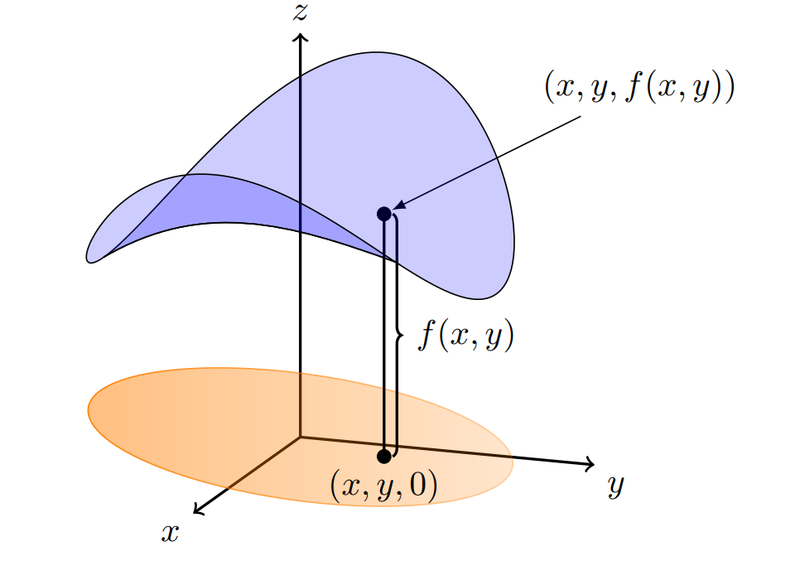
\includegraphics[scale=0.4]{surface.png}
  \caption{Eksplicitno podana ploskev.}
\end{figure}

\begin{zgled}
  Oglejmo si parametrizacijo sfere $S^2 (0, a)$ za $a > 0$.
  Naj bodo $x(\varphi, \theta) = a \cos \varphi \sin \theta$, 
  $y(\varphi, \theta) = a \sin \varphi \sin \theta$ in $z (\varphi, \theta) a \cos \theta$
  za $\varphi \in [0, 2\pi)$ in $\theta \in [0, \pi]$.
  Potem je $\vec{r}_\varphi = (-a \sin \varphi \sin \theta, a \cos \varphi \sin \theta, 0)$
  in $\vec{r}_\theta = (a \cos \theta \cos \theta, a \sin \varphi \cos \theta, -a \sin \theta)$.
  Od tod $$\vec{r}_\varphi \times \vec{r}_\theta = -a^2 \sin \theta(\cos \varphi \sin \theta, \sin \varphi \sin \theta, \cos \theta)$$
  in $|\vec{r}_\varphi \times \vec{r}_\theta| = a^2 \sin \theta$.
  Ta parametrizacija ni regularna v $\theta = 0$ in $\theta = \pi$.
  Fizično si to lahko predstavljamo, da krogle ne moremo "`zaviti"' v pravokoten list papirja.
\end{zgled}

\begin{zgled}
  Izračunajmo enačbo tangentne ravnine na $S^2 (0, 1)$ v točki $\varphi = \frac{\pi}{12}$
  in $\theta = \frac{\pi}{4}$.
  Vemo že, da je normala $\vec{n} = (\cos \varphi \sin \theta, \sin \varphi \sin \theta, \cos \theta)$.
  Če vse kotne funkcije vstavimo in poračunamo, dobimo 
  $\vec{n} = \left(\frac{\sqrt{3} + 1}{4}, \frac{\sqrt{3} - 1}{4}, \frac{\sqrt{2}}{2}\right)$.
  in enačba za ravnino je 
  $$\frac{\sqrt{3} + 1}{4} x + \frac{\sqrt{3} - 1}{4}y + \frac{\sqrt{2}}{2}z = 1.$$
\end{zgled}

\subsubsection{Merjenje na ploskvi}

Denimo, da imamo ploskev $\Sigma$ s parametrizacijo $\vec{r}: D \subseteq \R^2 \to \Sigma$.
Želimo znati izračunati dolžine krivulj na $\Sigma$, kot med krivuljami na $\Sigma$ in 
površino ploskve.
Naj bo $\Gamma \subseteq \Sigma$ krivulja na $\Sigma$.
Potem je $\Gamma$ slika krivulje $\gamma$ v $D$.
Naj bo $t \mapsto (u(t), v(t))$ parametrizacija $\gamma$ in posledično 
$t \mapsto \vec{r}(u(t), v(t))$ parametrizacija $\Gamma$.
Če odvajamo, dobimo $\frac{d}{dt} (\vec{r} (u(t), v(t))) = \vec{r}_u \dot{u} + \vec{r}_v \dot{v}$.
Sedaj je 
\begin{align*}
  |\vec{r}_u \dot{u} + \vec{r}_v \dot{v}|^2 = (\vec{r}_u \cdot \vec{r}_u) \dot{u}^2 + 2 (\vec{r}_u \cdot \vec{r}_v) \dot{u} \dot{v} + (\vec{r}_v \vec{r}_v) \dot{v}^2
\end{align*}
in definiramo $E = |\vec{r}_u|^2$, $F = \vec{r}_u \vec{r}_v$ in $G = |\vec{r}_v|^2$.
Potem se naša formula glasi $$l(\Gamma) = \int_\alpha ^\beta \sqrt{E\dot{u}^2 + 2F \dot{u} \dot{v} + G \dot{v}^2}\, dt.$$
Definirajmo kvadratno formo, ki preslika $(u, v)$ v 
$$\sprod{\begin{bmatrix}
  E & F\\
  F & G
\end{bmatrix} \begin{bmatrix}
  u \\ v
\end{bmatrix}}{\begin{bmatrix}
  u \\ v
\end{bmatrix}}.$$
Tej kvadratni formi pravimo 1. fundamentalna forma ploskve $\Sigma$.
Dokažemo lahko, da je ta matrika pozitivno definitna.
Takoj vidimo, da je $E = \vec{r}_u \cdot \vec{r}_u > 0$
in $F = \vec{r}_v \cdot \vec{r}_v > 0$.
Nadalje je njena determinanta enaka 
$$EG - F^2 = |\vec{r}_u|^2 |\vec{r}_v|^2 - (\vec{r}_u \cdot \vec{r}_v)^2 > 0,$$
kjer smo uporabili Cauchy-Schwartzevo neenakost.
Ker pa sta $\vec{r}_u$ in $\vec{r}_v$ linearno neodvisna, pa imamo tudi strogo neenakost.
Hkrati pa sledi 
$$(\vec{r}_u \dot{u} + \vec{r}_v \dot{v}) \cdot (\vec{r}_u \dot{u} + \vec{r}_v \dot{v}) = E \dot{u}^2 + 2F \dot{u} \dot{v} + G \dot{v}^2 \geq 0$$
za vsak par $(\dot{u}, \dot{v})$. Ta izraz je enak $0$ natanko tedaj,
ko je $\vec{r}_u \dot{u} + \vec{r}_v \dot{v} = 0$,
kar pa se lahko zgodi natanko takrat, ko je $\dot{u} = \dot{v} = 0$,
saj sta $\vec{r}_u$ in $\vec{r}_v$ v vsaki točki linearno neodvisna.

\begin{zgled}
  Vzemimo $S^2 (0, a)$.
  Potem je $\vec{r} (\varphi, \theta) = (a \cos \varphi \sin \theta, a \sin \varphi \sin \theta, a \cos \theta)$.
  Potem sta odvoda $r_\varphi = (-a \sin \varphi \sin \theta, a \cos \varphi \sin \theta, 0)$
  in $r_\theta = (a \cos \varphi \cos \theta, a \sin \varphi \cos \theta, -a \sin \theta)$.
  Potem po prejšnji izpeljavi dobimo $E = a^2 \sin^2 \theta$, $F = 0$ in $G = a^2$.
  Tako dobimo formulo za dolžino v obliki eliptičnega integrala: $l = \int_\alpha ^\beta a \sqrt{\sin^2 t + 1}\, dt \approx 3.82 a$. 
\end{zgled}

S pomočjo prve fundamentalne forme lahko izrazimo kot med krivuljama na $\Sigma$.
Naj bosta $\Gamma_1, \Gamma_2$ krivulji na $\Sigma$, ki se sekata v točki 
$p_0 \in \Sigma$. Naj bosta $\gamma_1, \gamma_2$ izražavi $\Gamma_1$
in $\Gamma_2$ v koordinatah na $D$ s parametrizacijama
$t \stackrel{\gamma_1}{\mapsto} (u_1 (t), v_1 (t))$ in $t \stackrel{\gamma_2}{\mapsto} (u_2 (t), v_2 (t))$.
Točka $p_0$ naj bo za $\gamma_1$ v sliki točke $t_1$ in za $\gamma_2$ v sliki točke $t_2.$ 
Tangenti na $\Gamma_1$ in $\Gamma_2$ v $p_0$ sta 
$(\vec{r}_u \dot{u}_1 + \vec{r}_v \dot{v}_1) (t_1) = \dvec{\Gamma}_1$
in $(\vec{r}_u \dot{u}_2 + \vec{r}_v \dot{v}_2) (t_2) = \dvec{\Gamma}_2$.
Kot $\alpha$ med $\Gamma_1$ in $\Gamma_1$ v $p_0$ zadošča enačbi 
$\cos \alpha = \frac{\dvec{\Gamma}_1 \cdot \dvec{\Gamma}_2}{|\dvec{\Gamma}_1| \cdot |\dvec{\Gamma}_2|}$.
Če je $\vec{r} (u_0, v_0) = p_0$ in sta $\dvec{\gamma}_1$ in $\dvec{\gamma}_2$
tangentna vektorja na $\gamma_1$ in $\gamma_2$ v $(u_0, v_0) \in D$.
Potem dobimo 
$$\dvec{\Gamma}_1 \cdot \dvec{\Gamma}_2 = \sprod{\begin{bmatrix}
  E & F\\ F & G
\end{bmatrix} (u_0, v_0) \dvec{\gamma}_1}{\dvec{\gamma}_2} \quad \mathrm{ter} \quad |\dvec{\Gamma}_j| = \sqrt{\sprod{\begin{bmatrix}
  E & F\\ F & G
\end{bmatrix} (u_0, v_0) \dvec{\gamma}_j}{\dvec{\gamma}_j}}.$$
Ti formuli sta seveda smiselni, ker je matrika pozitivno definitna.

\begin{zgled}
  Koordinatne krivulje na $\Sigma$ so slike premic $t \mapsto (t, v_0)$ ter $t \mapsto (u_0, t)$.
  Torej sta vektorja $\dvec{\gamma}_1 = (1, 0)$ in $\dvec{\gamma}_2 = (0, 1)$ ter
  kot med koordinatnima krivuljama je določen s formulo $\cos \alpha = \frac{F}{\sqrt{EG}}$.
\end{zgled}

\begin{opomba}
  Če je $F = 0$, imamo pravokotne krivočrtne koordinate.
  Primer je sfera $S^2(0, 1)$, kjer je
  $$\begin{bmatrix}
    E & F\\
    F & G
  \end{bmatrix} =
  \begin{bmatrix}
    \sin^2 \theta & 0\\
    0 & 1
  \end{bmatrix}.$$
\end{opomba}

\subsubsection{Površina ploskve}

Poskusimo intuitivno izpeljati formulo za površino krivulje.
Denimo, da imamo podano ploskev $\Sigma$, podano s parametrizacijo 
$\vec{r}: D \to \Sigma$.
Denimo, da imamo pravokotnik v $D$,
dan s točkami v ogliščih $v, v + \Delta v, u, u + \Delta u \in D$.
Potem lahko z Lagrangevim izrekom sliko tega pravokotnika aproksimiramo s paralelogramom,
danim
z vektorjema $\vec{r}_u (u, v) \Delta u = \vec{r}(u + \Delta u, v) - \vec{r}(u, v)$
in $\vec{r}_v (u, v) \Delta v = \vec{r}(u, v + \Delta v) - \vec{r}(u, v)$.
Sedaj uporabimo identiteto 
$(\vec{a} \times \vec{b}) \cdot (\vec{c} \times \vec{d}) = (\vec{a} \vec{c}) (\vec{b} \vec{d}) - (\vec{a} \vec{d}) (\vec{b} \vec{c})$
in dobimo 
\begin{align*}
  |\vec{r}_u \times \vec{r}_v |^2 &= (\vec{r}_u \times \vec{r}_v) \cdot (\vec{r}_u \times \vec{r}_v)\\
  &= (\vec{r}_u \cdot \vec{r}_u) (\vec{r}_v \cdot \vec{r}_v) - (\vec{r}_u \cdot \vec{r}_v) (\vec{r}_u \cdot \vec{r}_v)\\
  &= EG - F^2.
\end{align*}
Torej je ploščina iskanega paralelograma 
$$|\vec{r}_u \times \vec{r}_v| \Delta u \Delta v = \sqrt{EG - F^2} \Delta u \Delta v.$$

\begin{definicija}
  Površina ploskve z regularno $C^1$ parametrizacijo $\vec{r}: D \to \Sigma$
  je $$P(\Sigma) = \iint_D |\vec{r}_u \times \vec{r}_v|\, du\, dv = \iint_D \sqrt{EG - F^2}\, du\, dv.$$
\end{definicija}

\begin{opomba}
  Množice $E \subseteq D$ z mero $0$ ne vplivajo na vrednost integrala.
\end{opomba}

\begin{posledica}
  Če je $\Sigma = \{(x, y, f(x, y));\ (x, y)\in D\subseteq \R^2\}$ 
  graf $C^1$ funkcije $f$ na $D$, potem je njena površina 
  $$P(\Sigma) = \iint_D \sqrt{1 + f_x^2 + f_y^2}\, dx\, dy.$$
\end{posledica}

\begin{trditev}
  Vrednost integrala $\iint_D |\vec{r}_u \times \vec{r}_v|\, du\, dv$
  je neovisna od regularne parametrizacije $\Sigma$.
\end{trditev}

\begin{dokaz}
  Denimo, da imamo regularni parametrizaciji $\vec{r}: D \to \Sigma$
  in $\vec{\rho}: \Omega \to \Sigma$.
  Potem imamo difeomorfizem
  $\Phi : \Omega \to D$, dan s predpisom $\Phi = \vec{r}^{-1} \circ \vec{\rho}$.
  Naj bo $\Phi (s, t) = (U(s, t), V(s, t))$.
  Potem imamo odvod $\vec{\rho}_s \times \vec{\rho}_t = (\vec{r}_u U_s + \vec{r}_v V_s) \times (\vec{r}_u U_t + \vec{r}_v V_t) = (\vec{r}_u \times \vec{r}_v) (U_s V_t - V_s U_t)$.
  Od tod sledi $|\vec{\rho}_s \times \vec{\rho}_t| = |(\vec{r}_u \times \vec{r}_v) (\Phi (s, t))| |J\Phi|$.
  Sedaj pa lahko zapišemo 
  \begin{align*}
    \iint_D |\vec{r}_u \times \vec{r}_v|\, du\, dv &= \iint_\Omega |(\vec{r}_u \times \vec{r}_v) (\Phi(s, t))| |J\Phi (s, t)|\, ds\, dt\\
    &= \iint_\Omega |\vec{\rho}_s \times \vec{\rho}_t|\, ds\, dt. \qedhere
  \end{align*}
\end{dokaz}

\begin{zgled}
  Naj bo $f(x, y) = \frac{1}{2} (x^2 + y^2)$ in $f_x = x,\ f_y = y$.
  Naj bo $D = K(0, 1).$
  Potem je površina grafa $f$ na $D$ dana kot 
  $P = \iint_{D} \sqrt{1 + x^2 + y^2}\, dx\, dy = \int_0 ^{2 \pi} \int_0 ^1 r \sqrt{1 + r^2}\, dr\, d\varphi = \frac{2 \pi}{3} (2 \sqrt{2} - 1)$.
\end{zgled}

\begin{zgled}
  Vzemimo $S^2 (0, a)$. Ker je $E = a^2 \sin^2 \theta$, $F = 0$ in $G = a^2$.
  Torej je $EG - F^2 = a^4 \sin^2 \theta$.
  Površina te sfere je
  $P = \int_0 ^{2 \pi} \int_0 ^\pi a^2 \sin \theta\, d\theta\, d\varphi = 4 \pi a^2$. 
\end{zgled}

\begin{zgled}
  Schwartzev paradoks.
\end{zgled}

\clearpage
\section{VEKTORSKA ANALIZA}

\subsection{Vektorske diferencialne operacije}

V tem razdelku nekateri objekti dobijo fizikalno oziroma geometrijsko poimenovanje.
Funkciji iz $\R^3$ ali $\R^2$ tako pravimo skalarno polje,
preslikavi iz $R^3$ v $\R^3$ oziroma iz $R^2$ v $\R^2$ pa vektorsko polje.
Tipično so te preslikave zvezne in celo $C^1$.
Standardna ortonormirana baza $\R^3$ je $\vec{i}, \vec{j}, \vec{k}$
oziroma $\vec{e_1}, \vec{e_2}, \vec{e}_3$.
Za poljubno ortonormirano bazo $\vec{p}, \vec{q}, \vec{r}$ v prostoru $\R^3$
velja $|\vec{p}| = |\vec{r}| = |\vec{q}| = 1$
in $\vec{p} \cdot \vec{r} = \vec{q} \cdot \vec{r} = \vec{q} \cdot \vec{r} = 0$.
Če je mešani produkt $(\vec{p}, \vec{q}, \vec{r})$ pozitiven oziroma $\vec{r} = \vec{p} \times \vec{q}$, potem je ta ortonormirana baza 
pozitivno orientirana, sicer pa negativno orientirana. 

\begin{definicija}
  Naj bo $D \subseteq \R^3$ odprta.
  Zvezno funkcijo $u: D \to \R$
  imenujemo skalarno polje na $D$.
\end{definicija}

\begin{zgled}
  Primeri skalarnih polj v fiziki so na primer temperaturno polje 
  ali gostotna porazdelitev. Skalarno polje vsaki točki $T$ v $D$
  priredi skalar $u(T) \in \R$.
\end{zgled}

\begin{definicija}
  Naj bo $D \subseteq \R^3$ odprta.
  Zvezno preslikavo $\vec{R}: D \to \R^3$ imenujemo vektorsko polje na $D$.
\end{definicija}

\begin{zgled}
  Primeri vektorskega polja v fiziki so hitrostno polje tekočine ali gravitacija.
\end{zgled}

Če imamo dve ortonormirani bazi,
lahko skalarno ali vektorsko polje izrazimo v eni ali drugi.
Naj bo $U$ matrika, ki standardne bazne vektorje $\vec{e}_1, \vec{e}_2,  \vec{e}_3$ preslika zaporedno v ortonormirane bazne vektorje 
$\vec{p}, \vec{q}, \vec{r}.$ Vemo, da je $U$ ortogonalna.
Če imamo v standardni bazi koordinate $(x, y, z)$ 
in v $\vec{p}, \vec{q}, \vec{r}$ bazi koordinate $(\alpha, \beta, \gamma)$,
potem velja $$\begin{bmatrix}
  x \\ y \\ z
\end{bmatrix} = 
U \begin{bmatrix}
  \alpha \\ \beta \\ \gamma
\end{bmatrix}.$$
Če je $u : D \subseteq \R^3 \to \R$ skalarno polje v koordinatah $(x, y, z)$,
potem se v $(\alpha, \beta, \gamma)$ izraža kot 
$\tilde{u} (\alpha, \beta, \gamma) = u(U (\alpha, \beta, \gamma))$.
Podobno naredimo za vektorsko polje $\vec{R} : D \subseteq \R^3 \to \R^3$.
Le-to se v $(\alpha, \beta, \gamma)$ koordinatah izraža kot 
$\vec{\widetilde{R}} (\alpha, \beta, \gamma) = U^\top \vec{R} \circ U$.

\begin{zgled}\label{zgl:1}
  Vzemimo ortonormirano bazo $\vec{p} = \left(\frac{1}{\sqrt{2}}, 0, \frac{1}{\sqrt{2}}\right)$,
  $\vec{q} = (-\frac{1}{\sqrt{3}}, \frac{1}{\sqrt{3}}, \frac{1}{\sqrt{3}})$ 
  in $\vec{r} = (\frac{1}{\sqrt{6}}, \frac{2}{\sqrt{6}}, -\frac{1}{\sqrt{6}})$.
  Potem iz $(\alpha, \beta, \gamma)$ v standardne koordinate $(x, y, z)$
  slika matrika 
  $$U = \begin{bmatrix}
    \frac{1}{\sqrt{2}} & -\frac{1}{\sqrt{3}} & \frac{1}{\sqrt{6}}\\
    0 & \frac{1}{\sqrt{3}} & \frac{2}{\sqrt{6}}\\
    \frac{1}{\sqrt{2}} & \frac{1}{\sqrt{3}} & -\frac{1}{\sqrt{6}}
  \end{bmatrix}.$$
  Vzemimo vektorsko polje $\vec{R} = (x + 2y + 3z) (1, 1, 1)$
  in skalarno polje $u(x, y, z) = x$.
  Če to prevedemo v $(\alpha, \beta, \gamma)$ koordinate, dobimo 
  $\vec{\widetilde{R}} = \left(\frac{4}{\sqrt{2}}\alpha + \frac{4}{\sqrt{3}}\beta + \frac{2}{\sqrt{6}}\gamma\right)
  \left(\frac{2}{\sqrt{2}}, \frac{1}{\sqrt{3}}, \frac{2}{\sqrt{6}}\right)$
  in $\widetilde{u} (\alpha, \beta, \gamma) = \frac{1}{\sqrt{2}} \alpha - \frac{1}{\sqrt{3}}\beta + \frac{1}{\sqrt{6}}\gamma$.
\end{zgled}

\subsubsection{Smerni odvod skalarnega polja}

Naj bo $D \subseteq \R^3$ in $u : D \to \R$ skalarno polje.
Naj bo $\vec{s} \neq \vec{0}$ vektor in $\vec{p} \in D$.
Skalarni odvod skalarnega polja $u$ v smeri vektorja $\vec{s}$ v točki $\vec{p}$ 
obstaja, če obstaja limita 
$\lim_{t \to 0} \frac{u(\vec{p} + t \vec{s}) - u (\vec{p})}{t} = \frac{\partial u}{\partial \vec{s}} (\vec{p}).$
Če je $u \in C^1 (D)$, potem je po verižnem pravilu
$$\frac{\partial u}{\partial \vec{s}} (\vec{p}) = \frac{d}{dt} u(\vec{p} + t \vec{s}) \Big|_{t = 0} = (Du) (\vec{p}) \cdot\vec{s}.$$
Potem je $\frac{\partial u}{\partial \vec{s}} = (D u) (\vec{p}) \cdot \vec{s} = u_x s_x + u_y s_y + u_z s_z,$
kjer je $\vec{s} = (s_x, s_y, s_z)$ in $(Du) (\vec{p}) = \begin{bmatrix}
  u_x & u_y & u_z
\end{bmatrix} (\vec{p})$.
Naravno sledijo naslednje definicije.

\begin{definicija}
  Gradient skalarnega polja $u$ definiramo kot vektorsko polje $\mathrm{grad}\, u = (u_x, u_y, u_z)$.
  Operator nabla je diferencialni operator, ki se glede na bazo $\vec{e}_1, \vec{e}_2, \vec{e}_3$ glasi
  $\vec{\nabla} = \left(\frac{\partial}{\partial x}, \frac{\partial}{\partial y}, \frac{\partial}{\partial z}\right)$.
  Torej imamo $\mathrm{grad}\, u = \vec{\nabla} u = \left(\frac{\partial u}{\partial x}, \frac{\partial u}{\partial y}, \frac{\partial u}{\partial z}\right)$.
\end{definicija}

\begin{opomba}
  Ker je gradient $u$ vektorsko polje, ki pripada diferencialu 
  $Du$ v bazi $\vec{e}_1, \vec{e}_2, \vec{e}_3$, je dejansko dobro definirano 
  vektorsko polje na $D$, ki pripada skalarnemu polju $u$.
  Tako lahko vzamemo skalarno polje $u$ iz zgleda \ref{zgl:1}
  in se prepričamo, da je res $\vec{\widetilde{\nabla}} = U^\top (\vec{\nabla} u) U$.
\end{opomba}

Torej imamo z gradientom dano preslikavo $u \mapsto \mathrm{grad}\, u$,
ki slika iz prostora vseh $C^1$ skalarnih polj v prostor vseh $C$ vektorskih polj.
Naj bo $\vec{s}$ enotski vektor, torej $|\vec{s}| = 1$.
Potem je $\frac{\partial u}{\partial \vec{s}} = \grad u \times \vec{s} = |\grad u| |\vec{s}| \cos \theta$,
kjer je $\theta$ kot med $\grad u$ in $\vec{s}$.


\begin{trditev}
  Naj bo $u \in C^1 (D)$. V točki $\vec{p} \in D$ skalarno polje oziroma funkcija $u$
  najhitreje narašča v smeri $\mathrm{grad}\, u$ in najhitreje pada v smeri $-\mathrm{grad}\, u$.
\end{trditev}

\begin{opomba}
  V smereh, pravokotnih na gradient, se $u$ najpočasneje spreminja.
  Vemo, da je $\mathrm{grad}\, u$ pravokoten na nivojnice $u$.
\end{opomba}

\subsubsection{Divergenca vektorskega polja}

  Divergenco definiramo kot preslikavo iz prostora $C^1$ vektroskih polj
  v prostor $C$ skalarnih polj. 

\begin{definicija}
  Naj bo $\vec{R} : D \subseteq \R^3 \to \R^3$ vektorsko polje 
  razreda $C^1$ s predpisom $\vec{R} = (X, Y, Z)$
  Potem definiramo divergenco polja $\vec{R}$ kot skalrno 
  polje $\divg \vec{R} = X_x + Y_y + Z_z$.
  Z uporabo operatorja $\vec{\nabla}$
  to zapišemo kot $\divg \vec{R} = \vec{\nabla} \cdot \vec{R}$.
\end{definicija}

\begin{zgled}
  Kasneje bomo videli, da je to res dobro definirana operacija na vektorskem polju.
  Za zgled vzemimo že znano vektorsko polje $\vec{R} = (x + 2y + z) \cdot (1, 1, 1)$.
  Potem je divergenca enaka $\divg \vec{R} = 1 + 2 + 3 = 6$.
  Če spremenimo koordinate, dobimo $\vec{\widetilde{R}} = 
  \left(\frac{4}{\sqrt{2}}\alpha + \frac{4}{\sqrt{3}}\beta + \frac{2}{\sqrt{6}}\gamma \right) \left(\frac{2}{\sqrt{2}}, \frac{1}{\sqrt{3}}, \frac{2}{\sqrt{6}}\right)$.
  Ponovno je divergenca enaka $\divg \vec{\widetilde{ R}} = 6$.
\end{zgled}

Geometrijsko si lahko predstavljamo, da divergenca vektorskega polja $\vec{R}$
meri izvore oziroma ponore toka v posamezni točki.

\subsubsection{Rotor vektorskega polja}

Rotor definiramo kot preslikavo iz prostora 
$C^1$ vektorskih polj v prostor $C$ vektorskih polj.

\begin{definicija}
  Naj bo $\vec{R}: D \subseteq \R^3 \to \R^3$ vektorsko polje razreda $C^1$ s predpisom 
  $\vec{R} = (X, Y, Z)$ v običajnih koordinatah.
  Definiramo rotor vektorskega polja $\vec{R}$ kot 
  $$\rot \vec{R} = (Z_y - Y_z, X_z - Z_x, Y_x - X_y) = \vec{\nabla} \times \vec{R}.$$
\end{definicija}

\begin{zgled}
  Izkaže se, da je tudi rotor vektorskega polja $\R$ (skoraj)
  neodvisen od izbire koordinat.
  Vzemimo spet vektorsko polje iz 
  zgleda \ref{zgl:1}, torej $\vec{R} = (x + 2y + z) (1, 1, 1)$.
  Potem je $\rot \vec{R} = (-1, 2, -1)$.
  Če pa spremenimo koordinate, dobimo
  $\vec{\widetilde{R}} = 
  \left(\frac{4}{\sqrt{2}}\alpha + \frac{4}{\sqrt{3}}\beta + \frac{2}{\sqrt{6}}\gamma \right) \left(\frac{2}{\sqrt{2}}, \frac{1}{\sqrt{3}}, \frac{2}{\sqrt{6}}\right)$
  in $\rot \vec{\widetilde{R}} = \left(\frac{2}{\sqrt{2}}, -\frac{2}{\sqrt{3}}, - \sqrt{4}{\sqrt{6}}\right)$ in 
  izkaže se, da je v tem primeru $\rot \vec{\widetilde{R}} = - U^\top \rot \vec{R} U$.
  Negativen predznak se pojavi, ker baza $\vec{p}, \vec{q}, \vec{r}$ ni orientirana pozitivno.
  To pomeni, da velja $\det U = -1 = (\vec{p}, \vec{q}, \vec{r}) < 0$.
\end{zgled}

\begin{zgled}
  Naj bo $\vec{\omega} = (\omega_1, \omega_2, \omega_3)$ in $\vec{r} = (x, y, z)$.
  Vzemimo vektorsko polje $\vec{R} = \vec{\omega} \times \vec{r} = \left(\omega_2 z - \omega_3 y, \omega_3 x - \omega_1 z, \omega_1 y - \omega_2 x\right)$.
  Njegov rotor je $\rot \vec{R} = 2 \vec{\omega}$, torej rotor vektorskega polja meri vrtinčenje v okolici posamezne točke.
\end{zgled}

\begin{trditev}
  Naj bo $D$ odprta podmnožica $\R^3$, $u \in C^2 (D)$ skalarno polje
  in $\vec{R} \in C^2 (D)$ vektorsko polje.
  Tedaj:
  \begin{itemize}
    \item $\vec{\nabla} \times \vec{\nabla} u = \rot (\grad u) = \vec{0}$.
    \item $\vec{\nabla} \cdot \left(\vec{\nabla} \times \vec{R}\right) = \divg (\rot \vec{R}) = 0$.
  \end{itemize}
\end{trditev}

\begin{dokaz}
  To je posledica tega, da so mešani odvodi zvezni.
  \begin{align*}
    \rot (\grad u) = ((u_z)_y - (u_y)_z, (u_x)_z - (u_z)_x, (u_y)_x - (u_x)_y) = 0.
  \end{align*}
  Podobno tudi za drugo točko:
  \begin{equation*}
    \divg (\rot \vec{R}) = (Z_y - Y_z)_x + (X_z - Z_x)_y + (Y_x - X_y)_z = 0. \qedhere
  \end{equation*}
\end{dokaz}

\begin{opomba}
  Naj bo $\vec{R} : D \subseteq \R^3 \to \R^3$ vektorsko polje razreda $C^1$,
  da je $\rot \vec{R} = \vec{0}$.
  Ali obstaja $u \in C^2 (D)$, da je $\vec{R} = \grad u$.
  Podobno; če je $\divg \vec{G} = 0$, ali obstaja $\vec{R}$,
  da je $\vec{G} = \rot \vec{R}$?  
\end{opomba}

\begin{definicija}
  Vektorsko polje $\vec{R}$ je potencialno na odprti $D$, če obstaja $u \in C^1 (D)$,
  da je $\vec{R} = \grad u$.
  Potem je $u$ potencial za $\vec{R}$ (potreben pogoj za potencialno $\vec{R} \in C^1 (D)$ je $\rot \vec{R} = \vec{0}$).
  Podobno pravimo, da je vektorsko polje $\vec{R} \in C^1 (D)$
  irotacionalno ali nevrtinčno, če je $\rot \vec{R} = \vec{0}$ na $D$.
\end{definicija}

\begin{definicija}
  Definiramo Laplaceov operator $\triangle u = \divg \grad u = u_{xx} + u_{yy} + u_{zz}$.
  Funkcije, ki rešijo to enačbo, imenujemo harmonične funkcije.
\end{definicija}

\begin{opomba}
  Ta operator se pogosto pojavi v enačbah iz matematične fizike.
  Tako lahko napišemo toplotno enačbo kot $\triangle_{(x, y, z)} u = u_t$
  in valovno enačbo kot $\triangle_{(x, y, z)} u = u_{tt}$.
\end{opomba}

\begin{definicija}
  Množica $D \subseteq \R^3$ je konveksna, če za poljubni točki $\vec{a}, \vec{b} \in D$
  velja $\vec{a}t + \vec{b} (1 - t) \vec{b} \in D$ za $\forall t \in [0, 1]$.
  Pravimo tudi, $D$ zvezdasta, če obstaja taka točka $\vec{a}_0 \in D$, da za vsako 
  drugo točko $b \in D$ velja $t \vec{a}_0 + (1 - t)\vec{b} \in D$ za $\forall t \in [0, 1]$. 
  Konveksnost je močnejši pogoj, saj implicira zvezdastost.
\end{definicija}

\begin{trditev}
  Naj bo $D \subseteq \R^3$ zvezdasto območje\footnote{`območje' pomeni povezana odprta množica}.
  Naj bo $\vec{R} \in C^1 (D)$ vektorsko polje na $D$.
  \begin{enumerate}
    \item Če je $\rot \vec{R} = \vec{0}$ na $D$, je $\vec{R}$ potencialno vektorsko polje.
    \item Če je $\divg \vec{R} = 0$ na $D$, obstaja vektorsko polje $\vec{F} \in C^2 (D)$, da je $\vec{R} = \rot \vec{F}$
  \end{enumerate} 
\end{trditev}

\begin{zgled}\label{zgl:2}
  V splošnem, če $D$ ni zvezdasto, obrata zgornjih dveh trditev ne veljata.
  Konstruirajmo protiprimer za prvo točko.
  Vzemimo $D = \R^3 \setminus \{x = y = 0\}$ in polje 
  $\vec{R} (x, y, z) = \left( -\frac{y}{x^2 + y^2}, \frac{x}{x^2 + y^2}, 0 \right)$.
  Potem je $$\rot \vec{R} = \left(0, 0, \frac{2}{x^2 + y^2} - \frac{2x^2}{(x^2 + y^2)^2} -  \frac{2y^2}{(x^2 + y^2)^2}\right) = (0, 0, 0).$$
  Če bi potencial $u$ obstajal, bi imeli $u_x = - \frac{y}{x^2 + y^2}$,
  $u_y = \frac{x}{x^2 + y^2}$ in $u_z = 0$, torej bi veljalo  
  $$u(x, y, z) = \arctan \left(\frac{y}{x}\right) + A(y, z).$$
  Od tod pa sledi $u_y = \frac{x}{x^2 + y^2} + A_y = \frac{x}{x^2 + y^2}$,
  torej je $A_y = 0$. Vemo pa tudi, da je $A_z = 0$, torej je $A = A_0$
  konstantna funkcija. To pomeni, da je potencial $u$
  oblike $u(x, y, z) = \arctan \frac{y}{x} + A_0$.
  Ta funkcija pa ni dobro definirana na $\R^3 \setminus \{x = y = 0\}$.
\end{zgled}

\begin{definicija}
  Če za vektorsko polje $\vec{R}$ velja, da je $\divg \vec{R} = 0$, se imenuje solenoidalno polje. 
\end{definicija}

\begin{opomba}
  Naj bo $D$ zvezdasto območje.
  Koliko potencialov ima $\vec{R}$, če je $\rot \vec{R} = \vec{0}$?
  Denimo, da je $\grad u = \grad v = \vec{R}$ na $D$.
  Tedaj je tudi $\grad (u - v) = 0$,
  torej je $w = u - v$ taka funkcija, 
  da je $w_x = w_y = w_y = 0$ na $D$.
  Ker je $D$ zvezdasto območje, je tudi povezano. 
  Od tod pa sledi, da je $w$ konstantna funkcija,
  torej je $u = v + c$.
  Podobno kot nedoločen integral je tudi gradient določen 
  do konstante natančno.
\end{opomba}

\begin{opomba}
  Naj bo $\divg \vec{R} = 0$.
  Zanima nas, koliko rešitev enačbe $\rot \vec{F} = \vec{R}$ obstaja.
  Naj velja $\rot \vec{F}_1 = \rot \vec{F}_2 = \vec{R}$.
  Tedaj je $\rot (\vec{F}_1 - \vec{F}_2) = \vec{0}$.
  Potem obstaja $u \in C^2 (D)$, da je $\vec{F}_1 - \vec{F}_2 = \grad u$,
  torej se $\vec{F}_1$ in $\vec{F}_2$ razlikujeta za potencialno 
  vektorsko polje.
\end{opomba}

\begin{opomba}
  Naj bo $\vec{R} \in C^1 (D)$ vektorsko polje in $\divg \vec{R} = f$.
  Uporabimo dejstvo, da na $D$ obstajajo rešitve Poissonove enačbe 
  $\triangle u = f$ (analiza 4).
  Dobimo $u \in C^2 (D)$, da je $\triangle u = \divg (\grad u) = f = \divg \vec{R}$.
  Torej je $\divg (\vec{R} - \grad u) = 0$ in torej obstaja $F \in C^2 (D)$,
  da je $\vec{R} = \rot \vec{F} + \grad u = \vec{\nabla} \times \vec{F} + \vec{\nabla} \cdot u$
  na zvezdastem območju $D$.   
\end{opomba}

\begin{dokaz}
  Dokažimo prvo točko.
  Naj bo $\vec{R} = (X, Y, Z) \in C^1 (D)$ in $\rot \vec{R} = 0$. 
  Iščemo $u \in C^2 (D)$, da je $\grad u = \vec{R}$.
  Naj bo $(x, y, z) \in D$.
  Definiramo 
  $$u(x, y, z) = \int_0 ^1 \left(x X(tx, ty, tz) + y Y(tx, ty, tz) + z Z(tx, ty, tz)\right)\, dt.$$
  Tu za dobro definiranost uporabimo dejstvo, da je $D$ zvezna.
  Sedaj odvajamo:
  \begin{align*}
    u_x (x, y, z) &= \int_0 ^1 \left(X(tx, ty, tz) + x X_x \cdot t + y Y_x \cdot t + z Z_x \cdot t\right)\, dt\\
    &\stackrel{\rot \vec{R} = \vec{0}}{=} \int_0 ^1 \left(X + tx X_x + t y X_y + t z X_z\right)\, dt\\
    &= \int_0 ^1 \frac{d}{dt} \left(tX (tx, ty, tz)\right)\, dt\\
    &= tX (tx, ty, tz) \Big|_0 ^1 = X(x, y, z).
  \end{align*}
  Simetrično velja za $u_y = Y$ in $u_z = Z$.
  Sedaj dokažimo še drugo točko.
  Naj bo $\vec{R} = (X, Y, Z)$ in $\divg \vec{R} = X_x + Y_y + Z_z = 0$.
  Definiramo 
  \begin{align*}
    \alpha (x, y, z) &= \int_0 ^1 tX (tx, ty, tz)\, dt\\
    \beta (x, y, z) &= \int_0 ^1 tY (tx, ty, tz)\, dt\\
    \gamma (x, y, z) &= \int_0 ^1 tZ (tx, ty, tz)\, dt.
  \end{align*}
  Ker je območje $D$ zvezdasto, so te definicije smiselne.
  Iz predpostavk sledi, da je $\divg (\alpha, \beta, \gamma) = 0$.
  Sedaj definiramo $\vec{F} = (\alpha, \beta, \gamma) \times (x, y, z) = (z \beta - y \gamma, x \gamma - z \alpha, y \alpha - x \beta)$.
  Trdimo, da je $\rot \vec{F} = \vec{R}$.
  Dovolj je, če si pogledamo prvo komponento tega rotorja, ki je 
  \begin{align*}
    2 \alpha + x \alpha_x + y \alpha_y + z \alpha_z &= \int_0 ^1 \left(2 t X + t^2 x X_x + t^2 y X_y + t^2 z X_z\right)\, dt\\
    &= \int_0 ^1 \frac{d}{dt} \left(t^2 X (tx, ty, tz)\right)\, dt\\
    &= t^2 X (tx, ty, tz)\Big|_0 ^1 = X(x, y, z). \qedhere
  \end{align*}
\end{dokaz}

\begin{zgled}
  Naj bo vektorsko polje $\vec{R} = (y^2 z^3 + 2, 2xy z^3 + 1, 3xy^2 z^2)$.
  Potem imamo rotor 
  $$\rot \vec{R} = \left(6xyz^2 - 6 xyz^2, 3y^2 z^2 - 3y^2 z^2 , 2yz^3 - 2yz^3\right) = \vec{0}.$$
  Vsi možni potenciali tega vektorskega polja so oblike $u(x, y, z) = xy^2 z^3 + 2x + y + C$.
\end{zgled}

\begin{zgled}
  Za zgled poiščimo še `drugi' potencial.
  Naj bo $\vec{R}= (2y - 1, -1, 4x - 2xy) = \rot \vec{F}$.
  Takoj opazimo, da je res $\divg \vec{R} = 0$.
  Tako kot v dokazu definiramo funkcije $\alpha, \beta, \gamma$ in če poračunamo,
  dobimo $\alpha (x, y, z) = \frac{2}{3}y - \frac{1}{2}$, $\beta(x, y, z) = - \frac{1}{2}$
  in $\gamma (x, y, z) = \frac{4}{3} x - \frac{1}{2} xy$.
  Potem vpeljemo $\vec{F} = (\alpha, \beta, \gamma) \times (x, y, z)$ in dobimo želeni rezultat 
  $$\vec{F} = \left(-\frac{1}{2}z - \frac{4}{3}xy + \frac{1}{2}xy^2, \frac{4}{3} x^2 - \frac{1}{2}x^2 y - \frac{2}{3} yz + \frac{1}{2}z, \frac{2}{3}y^2 - \frac{1}{2}y + \frac{1}{2}x\right).$$
  Prepričamo se lahko, da je res $\rot \vec{F} = \vec{R}$.
\end{zgled}

\subsection{Orientacije krivulj in ploskev}

\subsubsection{Orientacije krivulj}

Naj bo $\Gamma \subseteq \R^3$ gladka krivlja.
Orientacija $\Gamma$ je zvezen izbor enotskega tangentnega vektorja vzdolž $\Gamma$ -- poimenujmo ga $\vec{T}$.
Če je $\Gamma$ povezana potem ima le dve možni orientaciji -- to sta $\vec{T}$ in $-\vec{T}$.
Vsaka krivulja pa je orientabilna.
Če je $\vec{r}: I \to \Gamma$ regularna parametrizacija, potem je $\vec{T} = \frac{\dvec{r}}{|\dvec{r}|}$
orientacija $\Gamma$, usklajena s parametrizacijo.
Č je $\Gamma$ gladka krivulja z dvema robnima točkama 
$\partial \Gamma = \{A, B\}$, potem orientacija $\Gamma$ 
porodi naravno orientacijo robnih točk $A, B$ in sicer tako,
da določi, katera od točk $A, B$ je začetna in katera končna točka krivulje.

Naj bo sedaj $\Gamma = \Gamma_1 \cup \dots \cup \Gamma_n$ odsekoma gladka krivulja, dana s končno unijo gladkih krivulj
$\Gamma_1, \dots, \Gamma_n$, kjer velja $\Gamma_j \cap \Gamma_l = \emptyset$ za $|j - l| \geq 2 \Mod{2}$ in
se krivulji $\Gamma_j, \Gamma_{j + 1}$ sekata le v eni od robnih točk, denimo $P_j$.
Zahtevamo še, da se krivulji $\Gamma_1$ in $\Gamma_n$ bodisi 
sekata v eni od robnih točk (naj bo to $P_n$) ali pa se sploh ne sekata.
Potem je orientacija odsekoma gladke krivulje $\Gamma = \Gamma_1 \cup \dots \cup \Gamma_n$
tak izbor orientacij na $\Gamma_1, \dots, \Gamma_n$,
da je končna točka $\Gamma_j$ enaka začetni točki $\Gamma_{j + 1}$
za vse $j = 1, \dots, n - 1$.
Če se sekata tudi $\Gamma_1$ in $\Gamma_n$, je končna točka $\Gamma_n$
enaka začetni točki $\Gamma_1$.

\subsubsection{Orientacije ploskev}

Vzemimo gladko ploskev $\Sigma \subseteq \R^3$.
Orientacija gladke ploskve $\Sigma$ je zvezen izbor enotske normale $\vec{N}$
na $\Sigma$.
Če je $\Sigma$ povezana in ima orientacijo $\vec{N}$, potem ima še orientacijo $-\vec{N}$.

\begin{zgled}
  Oglejmo si nekatere primere zlahka orientabilnih ploskev.
  \begin{itemize}
    \item Naj bo graf $G(f) = \{(x, y, f(x, y)),\ (x, y) \in D\}$.
  Potem imamo orientacijo $\vec{N} = \frac{(-f_x, -f_y, 1)}{\sqrt{1 + f_x^2 + f_y^2}}$, ki kaže navzgor.
    \item Naj bo $\vec{r} : D \to \Sigma$ regularna parametrizacija.
    Orientacija, ki jo $\vec{r}$ podaja na $\Sigma$, je $\vec{N} = \frac{\vec{r}_u \times \vec{r}_v}{|\vec{r}_u \times \vec{r}_v|}$.
    \item Orientacija sfere v izhodišču je $\vec{N} = \frac{\vec{r}}{|\vec{r}|}$.
    \item Orientacija plašča pokončnega valja, katerega osnovna ploskev ima središče v izhodišču, je $\vec{N}(x, y, z) = \frac{(x, y, 0)}{R}$.
    \item Če je $D$ odprta podmnožica v $\R^2$, je njena orientacija določena z normalo $\vec{N} = (0, 0, 1)$ (razen če ni drugače povedano).
    \item Primer neorientabilne ploskve je Möbiusov trak.
    Vendar pa se v $\R^3$ izkaže, da so vse ploskve, ki `nekaj omejujejo' orientabilne.
\end{itemize}
\end{zgled}

\begin{figure}
  \centering 
  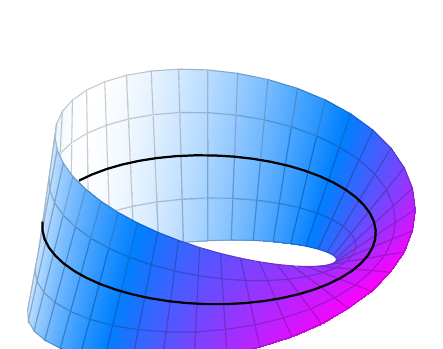
\begin{tikzpicture}
    \begin{axis}[
        hide axis,
        view={40}{40}
    ]
    \addplot3 [
        surf, shader=faceted interp,
        point meta=x,
        colormap/cool,
        samples=40,
        samples y=5,
        z buffer=sort,
        domain=0:360,
        y domain=-0.5:0.5
    ] (
        {(1+0.5*y*cos(x/2)))*cos(x)},
        {(1+0.5*y*cos(x/2)))*sin(x)},
        {0.5*y*sin(x/2)});
    
    \addplot3 [
        samples=50,
        domain=-145:180, % The domain needs to be adjusted manually, depending on the camera angle, unfortunately
        samples y=0,
        thick
    ] (
        {cos(x)},
        {sin(x)},
        {0});
    \end{axis}
    \end{tikzpicture}
  \caption{Möbiusov trak, primer neorientabilne ploskve v $\R^3$.}
\end{figure}

Vzemimo odsekoma gladko ploskev $\Sigma = \Sigma_1 \cup \dots \cup \Sigma_n$, ki je
končna unija gladkih omejenih ploskev 
$\Sigma_1, \dots, \Sigma_n$ z robovi $\partial \Sigma_1, \dots, \partial \Sigma_n$.
Naj bo $\partial \Sigma_i$ končna unija (odsekoma) gladkih sklenjenih krivulj
in presek $\Sigma_i$ in $\Sigma_j$
ali prazen ali pa vsebovan v robnih krivuljah $\partial \Sigma_i$ in $\partial \Sigma_j$.
Zahtevamo še to, da je presek treh izmed ploskev ali prazen ali pa točka.
Naj bo torej $\Sigma$ orientirana (z $\vec{N}$) ploskev z robom $\partial \Sigma$.
Temu robu podamo usklajeno oziroma koherentno orientacijo z $\vec{N}$.
Tedaj pravimo, da je $\partial \Sigma$ pozitivno orientirana glede na orientacijo $\Sigma$.
Opisno to naredimo tako, da če opazovalec hodi po $\partial \Sigma$
in ima glavo v smeri $\vec{N}$, potem hodi pozitivno, če je $\Sigma$ na njegovi levi strani.
Če je zaprtje $\overline{\Sigma}$ vsebovano v notranjosti večje gladke ploskve $\widetilde{\Sigma}$
in $\vec{N}$ podaja orientacijo $\overline{\Sigma}$, potem lahko v robni točki 
$p \in \partial \Sigma$ določimo enotsko zunanjo normalo $\vec{n}$ na $\overline{\Sigma}$
v $\widetilde{\Sigma}$. Potem je orientacija krivulje $\partial \Sigma$
podan z $\vec{T} = \vec{N} \times \vec{n}$.

\begin{opomba}
  Naj bo $D \subseteq \R^2 \subseteq \R^2 \times \{0\}$ odprta množica.
  Če ni drugače rečeno, je orientacija $D$ določena z $\vec{N} = (0, 0, 1)$.
\end{opomba}

Vrnimo se k orientaciji odsekoma gladke ploskve $\Sigma = \Sigma_1 \cup \dots \cup \Sigma_n$.
Če obstaja, je to tak izbor orientacij $\Sigma_1, \dots, \Sigma_n$,
da sta inducirani orientaciji na vsakem skupnem kosu robnima
$\partial \Sigma_i \cap \partial \Sigma_j$ nasprotni.

\subsection{Krivuljni integral}

Obravnavali bomo integral skalarnega polja po krivulji $\Gamma$
(tu orientacija ni pomembna) in integral vektorskega polja po orientirani krivulji.

\begin{definicija}
  Naj bo $\Gamma$ gladka omejena krivulja in zvezno skalarno polje 
$u: \Gamma \to \R$.
Naj bo $\vec{r} : [\alpha, \beta] \to \Gamma$ regularna parametrizacija.
Potem definiramo krivuljni integral kot 
$$\int_\Gamma u\, ds := \int_{\alpha} ^\beta u(\vec{r} (t))|\dvec{r} (t)|\, dt.$$
\end{definicija}

\begin{opomba}
  Po enakem sklepu, kot smo ga že naredili z vpeljavo novih koordinat v integral,
  je da definicija neodvisna od izbora regularne parametrizacije.
\end{opomba}

\begin{zgled}
  Izračunajmo težišče homogene žice v obliki polkroga s polmerom $R$.
  Seveda imamo regularno parametrizacijo $\vec{r} (t) = (R \cos t, R \sin t)$
  za $t \in [0, \pi]$. Ker je žica homogena, je njena gostota $\rho_0$ konstantna.
  Potem je $m = \rho_0 \int_\Gamma 1\, ds = \pi R \rho_0$ in 
  $y_T = \frac{1}{m} \int_\Gamma y \rho_0 \, ds = \frac{2 R}{\pi}$.
\end{zgled}

\begin{opomba}
  Če je $\Gamma$ odsekoma gladka krivulja $\Gamma = \Gamma_1 \cup \dots \cup \Gamma_n$,
  potem je $\int_\Gamma u\, ds = \int_{\Gamma_1} \, ds + \dots + \int_{\Gamma_n} u\, ds$.
\end{opomba}

\begin{definicija}
  Naj bo $\vec{\Gamma} = (\Gamma, \vec{T})$ orientirana gladka krivulja.
  Naj bo $\vec{r} : [\alpha, \beta] \to \Gamma$ regularna parametrizacija, usklajena z orientacijo 
  $\vec{T}$. Potem definiramo integral vektorskega polja po $\vec{\Gamma}$
  kot 
  $$\int_{\vec{\Gamma}} \vec{R}\, d\vec{r} = \int_\alpha ^\beta \vec{R} (\vec{r} (t))\cdot \dvec{r}(t)\, dt.$$
\end{definicija}

Takoj sledi 
\begin{align*}
  \int_{\vec{\Gamma}} \vec{R}\, d\vec{r} &= \int_\alpha ^\beta \vec{R} (\vec{r} (t)) \frac{\dvec{r} (t)}{|\dvec{r} (t)|} |\dvec{r} (t)|\, dt\\
  &= \int_\alpha ^\beta \vec{R} (\vec{r} (t)) \cdot \vec{T} |\dvec{r} (t)|\, dt\\
  &= \int_\Gamma (\vec{R} \cdot \vec{T})\, ds.
\end{align*}
Tokrat je integral $\vec{R}$ po $\vec{\Gamma}$ je neodvisen od regularne
parametrizacije $\Gamma$, ki ohranja orientacijo (oziroma je usklajena z dano orientacijo).
Če orientacijo obrnemo, se predznak intervalu spremeni: $\int_{-\vec{\Gamma}} \vec{R}\, d\vec{r} = \int_{\vec{\Gamma}} \vec{R}\, d\vec{r}$. 
Naj bo $\vec{R} = (X, Y, Z)$.
Potem je $\int_{\vec{\Gamma}} \vec{R}\, d\vec{r} = \int_{\vec{\Gamma}} (X, Y, Z)\, (dx, dy, dz) = \int_\Gamma (X\, dx + Y\, dy + Z\, dz)$.
Izrazu $\omega = X\, dx + Y\, dy + Z\, dz$ pravimo diferencialna 1-forma.

\begin{trditev}
  Naj bo $\vec{R} = \grad u$ zvezno potencialno vektorsko polje 
  na odprti množici $D \subseteq \R^3$ s potencialom $u \in C^1 (D)$.
  naj bo $\vec{\Gamma}$ orientiana odsekoma gladka krivulja v $D$ 
  z začetno točko $A$ in končno točko $B$.
  Potem je $\int_{\vec{\Gamma}} \vec{R}\, d\vec{r} = u(B) - u(A)$.
\end{trditev}

\begin{dokaz}
  Naj bo $D \subseteq \R^3$ odprta množica in $\vec{R} = \grad u$, kjer je $u \in C^1 (D)$.
Naj bo $\Gamma$ gladka oziroma odsekoma gladka orientirana krivulja v $D$.
Potem je 
\begin{align*}
  \int_{\vec{\Gamma}} \vec{R}\, d\vec{r} &= \int_{\vec{\Gamma}} u_x\, dx + u_y\, dy + u_z\, dz\\
  &= \int_{\alpha} ^\beta  (u_x \dot{x} + u_y \dot{y} + u_z \dot{z})\, dt\\
  &= \int_\alpha ^\beta \grad u \cdot \dvec{r}\, dt\\
  &= \int_\alpha ^\beta (Du)\dvec{r}\, dt\\
  &= \int_\alpha ^\beta \frac{d}{dt} \left(u(\vec{r} (t))\right)\, dt\\
  &= u(\vec{r} (\alpha)) - u (\vec{r} (\beta)). \qedhere
\end{align*}
\end{dokaz}

Vrednost integrala je odvisna torej le od razlike potencialov.

\begin{opomba}
  Če je $D$ zvezdasto območje, potem je 
  $\vec{R} \in C^1 (D)$ potencialno vektorsko polje natanko tedaj, ko je $\rot \vec{R} = \vec{0}$.
  Spomnimo se dokaza: podali smo daljico od točke $(0, 0, 0)$ do poljubne točke $(x, y, z)$ z regularno
  parametrizacijo $\vec{r}(t) = (tx, ty, tz)$ in 
  za potencial $u$ definirali $u(x, y, z) = \int_0 ^1 \vec{R}(\vec{r} (t)) \cdot \dvec{r} (t)\, dt$,
  kar je natanko integral vektorskega polja $\vec{R}$ po daljici od $(0, 0, 0)$ do $(x, y, z)$. 
\end{opomba}

\begin{izrek}
  Naj bo $D \subseteq \R^3$ odprto območje in $\vec{R} : D \to \R^3$ zvezno vektorsko polje.
  Potem so naslednje izjave ekvivalentne.
  \begin{enumerate}
    \item Vektorsko polje $\vec{R}$ je potencialno na $D$, torej obstaja $C^1$ skalarno polje $u$ na 
    $D$, da je $\vec{R} = \grad u$.
    \item Integral $\vec{R}$ je neodvisen od poti, torej za poljubni dve točki $A, B \in D$
    in poljubni odsekoma gladki orientirani krivulji $\Gamma_1$ in $\Gamma_2$ v $D$,
    ki gresta od $A$ do $B$, velja $\int_{\vec{\Gamma}_1} \vec{R}\, d\vec{r} = \int_{\vec{\Gamma}_2} \vec{R}\, d\vec{r}$.
    \item Za poljubno sklenjeno odsekoma gladko orientirano krivuljo $\vec{\Gamma} \subseteq D$ velja $\oint_{\vec{\Gamma}} \vec{R} d\vec{r} = 0$.
  \end{enumerate}
\end{izrek}

\begin{dokaz}
  Dokažimo najprej $(3) \Rightarrow (2)$.
  Naj bosta $\vec{\Gamma}_1$ in $\vec{\Gamma}_2$ orientirani krivulji 
  iz točke $A$ v točko $B$. Potem je $\vec{\Gamma} = \vec{\Gamma}_1 \cup (-\vec{\Gamma}_2)$
  sklenjena odsekoma zvezna krivulja. Sedaj imamo 
  \begin{align*}
    \oint_{\vec{\Gamma}} \vec{R}\, d\vec{r} &=\int_{\vec{\Gamma}_1 \cup (-\vec{\Gamma}_2)} \vec{R}\, d\vec{r}\\
    &= \int_{\vec{\Gamma}_1} \vec{R}\, d\vec{r} + \int_{-\vec{\Gamma}_2} \vec{R}\, d\vec{r}\\
    &= \int_{\vec{\Gamma}_1} \vec{R}\, d\vec{r} - \int_{\vec{\Gamma}_2} \vec{R}\, d\vec{r}\\
    &= 0
  \end{align*}
  in smo dokazali. Sedaj dokažimo še $(2) \Rightarrow (1)$.
  Ker je $D$ povezana, je s potmi povezana.
  Naj bo $A_0 \in D$ in $T(x, y, z) \in D$.
  Naj bo $\vec{\Gamma} \subseteq D$ orientirana zvezna krivulja, ki se začne v točki $A_0$
  in konča v $T$. Definiramo $u(T) = u(x, y, z) = \int_{\vec{\Gamma}} \vec{R}\, d\vec{r}$ 
  in to je po predpostavki neodvisno od izbora $\vec{\Gamma}$.
  Če je $\vec{R} = (X, Y, Z)$, potem trdimo, da je $u_x = X$,
  $u_y = Y$ in $u_z = Z$. 
  Sedaj definiramo $\vec{\widetilde{\Gamma}}$ kot unijo krivulje $\vec{\Gamma}$
  in daljice od $(x, y, z)$ in $(x + h, y, z)$.
  \begin{align*}
    u_x (x, y, z) &= \lim_{h \to 0} \frac{u(x + h, y, z) - u(x, y, z)}{h}\\
    &= \frac{1}{h} \left( \int_{\vec{\tilde{\Gamma}}} \vec{R}\, d\vec{r} - \int_{\vec{\Gamma}} \vec{R}\, d\vec{r} \right)\\
    &= \frac{1}{h} \int_{T} ^{\widetilde{T}} \vec{R}\, d\vec{r}\\
    &= \int_0 ^1 X(x+ht, y, z)\, dt,
  \end{align*}
  kjer smo v zadnjem koraku vpeljali parametrizacijo $\vec{r} (t) = (x + ht, y, z)$.
  Sedaj pa po zveznosti integrala s parametrom sledi želen zaključek:
  \begin{equation*}
    \lim_{h \to 0} \frac{u(x + h, y, z) - u(x, y, z)}{h} = \lim_{h \to 0} \int_0 ^1 X(x+ht, y, z)\, dt = X(x, y, z). \qedhere 
  \end{equation*}
\end{dokaz}

\begin{zgled}
  Spomnimo se zgleda \ref{zgl:2}
  in vzemimo polje 
  $\vec{R} (x, y, z) = \left( -\frac{y}{x^2 + y^2}, \frac{x}{x^2 + y^2}, 0 \right)$
  na $D = \R^3 \setminus \{x = y = 0\}$.
  Naj bo $\Gamma$ krožnica $x^2 + y^2 = 1,\ z = 0$.
  Glede na krog $x^2 + y^2 = 1,\ z = 0$ je njena parametrizacija 
  $\vec{r}(t) = (\cos t, \sin t)$ za $t \in [0, 2\pi]$.
  To je sklenjena krivulja in če bi $\vec{R}$ bilo potencialno polje,
  bi moralo veljati $\oint_\Gamma \vec{R} \, d\vec{r} = 0$.
  Vendar pa imamo 
  \begin{align*}
    \int_\Gamma \vec{R}\, d\vec{r} &= \int_0 ^{2 \pi} ((-\sin t) (-\sin t) + (\cos t) (\cos t))\, dt\\
    &= 2 \pi \neq 0 
  \end{align*}
  in pridemo v protislovje.
\end{zgled}

\subsection{Ploskovni integral}

\begin{definicija}
  Naj bo $\Sigma$ gladka ploskev s parametrizacijo $\vec{r} : D_{s, t} \subseteq\R^2 \to \Sigma$.
  Naj bo $u: \Sigma \to \R$ zvezno skalarno polje. Potem definiramo 
  $$\iint_\Sigma u\, dS := \iint_D u(\vec{r}(s, t)) \sqrt{EG - F^2}\, ds\, dt = \iint_D u(\vec{r}(s, t)) |\vec{r}_s \times \vec{r}_t|\, ds\, dt.$$
\end{definicija}

\begin{opomba}
  Ta vrednost je neodvisna od izbora regularne parametrizacije.
\end{opomba}

Če je $\Sigma = \Sigma_1 \cup \dots \cup \Sigma_n$ odsekoma gladka ploskev, velja $\iint_\Sigma u\, dS = \sum_{i = 1}^n \iint_{\Sigma_i} u\, dS$.

\begin{zgled}
  Naj bo $S^2(0, R)$ homogena sfera s ploščinsko gostoto $\rho_0$.
  Parametriziramo jo s $\vec{r} (\varphi, \theta) = (R\cos \varphi \sin \theta, R \sin \varphi \sin \theta, R \cos \theta)$
  in vemo že, da je $\sqrt{EG - F^2} = R^2 \sin \theta.$
  Vztrajnostni moment te sfere je
  \begin{align*}
    J_z &= \iint_{\Sigma} \rho_0 (x^2 + y^2)\, dS\\
    &= \rho_0 \int_0 ^{2\pi} \left(\int_0 ^\pi R^4 \sin^3 \theta\, d\theta\right)d\varphi\\
    &= 2 \pi \rho_0 R^4 \int_0 ^\pi \sin \theta (1 - \cos^2 \theta) d\theta\\
    &= 2 \pi R^4 \rho_0 \int_{-1} ^1 (1 - t^2)\, dt\\
    &= 2 \pi R^4 \rho_0 \frac{4}{3} = \frac{2}{3} m R^2.
  \end{align*}
\end{zgled}

\begin{definicija}
  Naj bo $\Sigma$ orientirana ploskev in $\vec{N}$ zvezna enotska normala na $\Sigma$,
  torej $\vec{\Sigma} = (\Sigma, \vec{N})$. Potem definiramo integral 
  $$\iint_{\vec{\Sigma}} \vec{R}\, d\vec{S} := \iint_{\Sigma} (\vec{R} \cdot \vec{N})\, dS.$$
\end{definicija}

\begin{opomba}
  Integral po $\Sigma$ z nasprotno orientacijo $-\vec{N}$ je enak $-\iint_{\vec{\Sigma}} \vec{R}\, d\vec{S} = \iint_{-\vec{\Sigma}} \vec{R}\, d\vec{S}$.
\end{opomba}

Izračunajmo integral v parametrizaciji $\vec{r} : D_{(s, t)} \to \Sigma$.
Ta parametrizacija je usklajena z orientacijo $\vec{N} = \frac{\vec{r}_s \times \vec{r}_t}{|\vec{r}_s \times \vec{r}_t|}$.
Potem imamo integral 
\begin{align*}
  \iint_{\vec{\Sigma}} \vec{R}\, d\vec{S} &= \iint_{\Sigma} (\vec{R} \cdot \vec{N}) \cdot dS\\
  &= \iint_D (\vec{R} \cdot \vec{N}) |\vec{r}_s  \times \vec{r}_t|\, ds\, dt\\
  &= \iint_D (\vec{R}, \vec{r}_s, \vec{r}_t)\, ds\, dt\\
  &= \iint_D \vec{R} \cdot (\vec{r}_s \times \vec{r}_t)\, ds\, dt.
\end{align*}

Če je $\Sigma = \Sigma_1 \cup \dots \cup \Sigma_n$ odsekoma gladka in 
orientirana, je $\iint_{\vec{\Sigma}} \vec{R}\, d\vec{S} = \sum_{i = 1}^n \iint_{\vec{\Sigma}_i} \vec{R}\, d\vec{S}$. 

\begin{opomba}
  Omenili smo že 1-formo in $\int_{\vec{\Gamma}} \vec{R}\, d\vec{r} = \int_{\vec{\Gamma}} X\, dx + Y\, dy + Z\, dz.$
  Sedaj lahko vpeljemo še 2-formo:
  $$\iint_{\vec{\Gamma}} \vec{R}\, d\vec{S} = \iint_\Sigma X\, dy \wedge dz + Y\, dz \wedge dx + Z\, dx \wedge dy.$$
\end{opomba}

\begin{zgled}\label{zgl:3}
  Naj bo vektorsko polje 
  $$\vec{R} = \left(\frac{x}{(x^2 + y^2 + z^2)^{\frac{3}{2}}}, \frac{y}{(x^2 + y^2 + z^2)^\frac{3}{2}}, \frac{z}{(x^2 + y^2 + z^2)^\frac{3}{2}}\right).$$
  Hitro lahko preverimo, da je njegova divergenca $\divg \vec{R} = 0$.
  Če to vektorsko polje integriramo po sferi $S(0, R)$, dobimo 
  \begin{align*}
    \iint_{\vec{S^2}(0, R)} \vec{R}\, d\vec{S} &= \int_{S^2 (0, R)} \frac{(x, y, z)}{R^3} \frac{(x + y+ z)}{R}\, dS\\
    &= \frac{1}{R^2} \iint_{\vec{S^2}(0, R)} 1\, dS\\
    &= \frac{1}{R^2} 4 \pi R^2 = 4 \pi \neq 0.  
  \end{align*}
  Na ta primer se bomo še sklicali, ko bomo dokazali, da to vektorsko polje nima "`vektorskega"' potenciala.
\end{zgled}

\subsection{Integralski izreki}

Naj bo $M$ orientirana mnogoterost z robom $\partial M$ in 
naj ima ta rob usklajeno orientacijo. Izreki, ki jih bomo obravnavali,
imajo strukturo $\int_M d\omega = \int_{\partial M} \omega$ (posplošeni Stokesov izrek).

\begin{izrek}[Gauss]
  Naj bo $D$ omejena odprta množica v $\R^3$ z odsekoma gladkim robom, sestavljenim iz končnega 
  števila odsekoma gladkih sklenjenih ploskev, orientiranih z zunanjo normalo glede na $D$.
  Naj bo $\vec{R} \in C^1 (\overline{D})$ vektorsko polje. Tedaj je 
  $$\iint_{\partial D} \vec{R} \, d\vec{S} = \iiint_{D} \divg \vec{R}\, dV.$$ 
\end{izrek}

\begin{izrek}[Greenova formula]
  Naj bo $D \subseteq \R^2$ omejena odprta množica z odsekoma gladkim robom,
  sestavljenem iz končnega števila odsekoma gladkih sklenjenih krivulj, orientiranih 
  pozitivno glede na $D$. Naj bosta $X, Y \in C^1 (\overline{D})$.
  Tedaj je 
  $$\int_{\partial D} X\, dx + Y\, dy = \iint_D (Y_x - X_y)\, dx\, dy.$$
\end{izrek}

\begin{izrek}[Stokes]
  Naj bo $\Sigma \subseteq \R^3$ omejena odsekoma gladka orientirana ploskev
  z robom, sestavljenim iz končnega števila odsekoma gladkih sklenjenih krivulj,
  orientiranih skladno z $\Sigma$. Naj bo $\vec{R} \in C^1 (\overline{D})$ vektorsko polje.
  Tedaj je 
  $$\int_{\partial \vec{\Sigma}} \vec{R}\, d\vec{r} = \iint_{\vec{\Sigma}} \rot \vec{R} \cdot d\vec{S}.$$
\end{izrek}

\begin{figure}[]
  \centering
  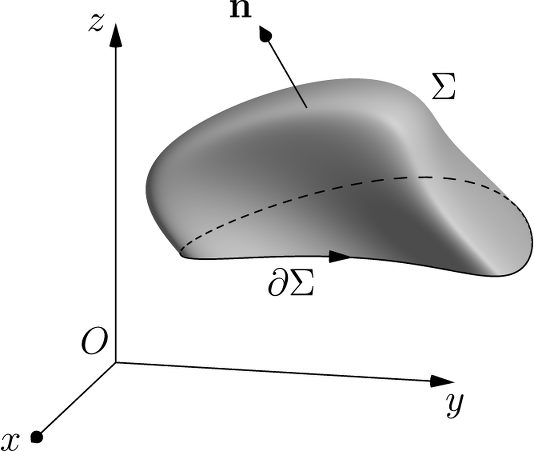
\includegraphics[scale=6.0]{stokes.png}
  \caption{Stokesov izrek.}
\end{figure}

\begin{opomba}
  Stokesov izrek implicira Greenovo funkcijo.
\end{opomba}

\begin{zgled}
  Naj bo $\vec{R} (x, y, z) = (x, y, z)$ na $D = K(0, R_0)$ in $\divg \vec{R} = 3$.
  Potem je $$\iiint_D \divg \vec{R} \, dV = 3 V(D) = 4 \pi R_0^3.$$
  Po drugi strani pa je $$\iint_{\partial D} \vec{R}\, d\vec{S} = \iint_{\partial D} \vec{r} \cdot \frac{\vec{r}}{r_0} \, dS = R_0 \iint_{\partial D} 1\, dS = R_0 (4 \pi R_0^2)$$
  in se ujema z Gaussovim izrekom.
\end{zgled}

\begin{zgled}
  Naj bo $D = \{(x, y) \in \R^2;\ 1 \leq x^2 + y^2 \leq 9\}$
  in $X (x, y)= -y,\ Y(x, y) = x$.
  Po eni strani imamo $$\iint_D (1 - (-1))\, dx\, dy = 2 P(D) = 2\pi (9 -1) = 16 \pi.$$
  Po drugi strani pa vpeljemo parametrizacijo $t \mapsto (3 \cos t, 3\sin t)$ za $t \in [0, 2\pi)$ in je integral prve krivulje 
  $$\int_{S^1(0, 3)} X\, dx + Y\, dy = \int_{S^1(0, 3)} (X, Y)\, d\vec{r} = \int_0 ^{2 \pi} 9\, dt = 18 \pi.$$
  Za drugo krivuljo pa vpeljemo parametrizacijo $t \mapsto (\cos t, \sin t)$ za $t$ od $2 \pi$ do $0$.
  Tokrat dobimo $\int_{S^1 (0, 1)} X\, dx + Y\, dy = \int_{2 \pi} ^0 1\, d\varphi = - 2\pi$
  in rezultat se ujema z Greenovo formulo.
\end{zgled}

\begin{zgled}
  Naj bo polsfera $\Sigma = \{(x, y, z) \in \R^3;\ x^2 + y^2 + z^2 = R_0^2,\ z \geq 0\}$,
  orientiran z normalo $\vec{N} = (0, 0, 1)$. Vzemimo vektorsko polje $\vec{R} = (zy, x, x - y + z)$
  in $\rot \vec{R} = (-1, y - 1, 1 - z)$. Potem je 
  \begin{align*}
    \iint_{\Sigma} \rot{\vec{R}}\, d\vec{S} &= \frac{1}{R_0} \iint_{\Sigma} (-1, y - 1, 1 - z) (x, y, z)\, dS\\
    &= \frac{1}{R_0} \iint_{\Sigma} (-x + y^2 - y+ z - z^2)\, dS\\
    \intertext{in ko vpeljemo sferične koordinate ter $dS = R_0^2 \sin \theta\, d\theta\, d\varphi$, dobimo}
    &= \pi R_0 ^2 \left(R_0 \left(1 - \frac{1}{3}\right) + 1 - \frac{2R_0}{3}\right) = \pi R_0^2. 
  \end{align*}
  Po drugi strani pa imamo 
  \begin{align*}
    \int_{\partial \Sigma} \vec{R}\, d\vec{r} &= \int_{\partial \Sigma} (zy, x, x - y)\, d\vec{r}\\ 
    &= \int_0 ^{2\pi} (0, R_0 \cos t, R_0 \cos t - R_0 \sin t) R_0 (-\sin t, \cos t, 0)\, dt\\
    &= R_0^2  \int_0 ^{2\pi} \cos^2 t\, dt = \pi R_0^2.
  \end{align*}
\end{zgled}

\begin{zgled}
  Vrnimo se k vektorskemu polju $\vec{R}$ iz zgleda \ref{zgl:3} na sferi $S^2(0, R)$.
  Denimo, da obstaja tako vektorsko polje $\vec{F}$, da je $\vec{R} = \rot \vec{F}$.
  Potem bi po Stokesovem izreku sledilo 
  $$0 = \int_{\partial \vec{S^2}(0, R)} \vec{F} d\vec{r}= \iint_{\vec{S^2}(0, R)} \rot \vec{F}\, d\vec{S} = 4\pi \neq 0$$
  in smo prišli v protislovje.
\end{zgled}

\subsection{Skica dokazov izrekov}

Najprej dokažimo, da Gaussov izrek v $\R^2$ implicira Greenovo formulo.
Denimo, da $D \subseteq \R^2$ ustreza pogojem Greenove formule.
Naj bosta $X, Y \in C^1 (\overline{D})$ in definirajmo $\vec{R} = (X, Y)$ ter 
$\vec{\widetilde{R}} = (Y, -X)$. Na slednjem vektorskem polju 
uporabimo Gaussov izrek za $\R^2$: $\int_{\partial D} \vec{\widetilde{R}} \cdot \vec{N} ds = \iint_D (Y_x - X_y)\, dx\, dy$.
Sedaj vidimo, da če je $\vec{N} = (N_x, N_y)$, potem $\vec{T} = (-N_y, N_x)$
in $\vec{\widetilde{R}} \cdot \vec{N} = \vec{R} \cdot \vec{T}$ in smo končali:
$$\int_{\partial D} \vec{R} \cdot \vec{T} ds = \int_{\partial D} \vec{\widetilde{R}} \cdot \vec{N} ds = \iint_D (Y_x - X_y)\, dx\, dy.$$
Sedaj dokažimo, da Greenova formula implicira Stokesov izrek.
Naj bo $\Sigma = \Sigma_1 \cup \Sigma_2$ in $\vec{N}$ orientacija $\Sigma$.
Če je $\Gamma_0 = \partial \Sigma_1 \cap \partial \Sigma_2$,
je rob $\partial \Sigma = (\partial \Sigma_1 \cup \partial \Sigma_2) \setminus \Gamma_0.$
Lahko se prepričamo, da velja $\int_{\partial \Sigma} \vec{R}\, d\vec{r} = \int_{\partial \Sigma_1} \vec{R}\, d\vec{r} + \int_{\partial {\Sigma}_2} \vec{R}\, d\vec{r}$,
dela integralov po $\Gamma_0$ uničita zaradi nasprotnih orientacij.
Na podlagi te ugotovitve je dovolj pokazati Stokesov izrek
za dele ploskve $\Sigma$, ki jih nato sestavimo skupaj.
Naj bo $\Sigma$ graf na $(x, y)$ ravnino, torej 
$$\Sigma = \{(x, y, f(x, y));\ (x, y) = D \subseteq \R^2\},$$
kjer je $D$ omejena z odsekoma gladkim robom in je $f$ $C^2$ funkcija.
Denimo, da je orientacija $\Sigma$ dana z $\frac{(-f_x, -f_y, 1)}{\sqrt{1 + f_x^2 + y^2}}$.
Upoštevamo še, da je $\partial \Sigma$ parametriziran nad $\partial D$
z $(x, y, f(x, y))$ in je zato $dz = f_x\, dx + f_y\, dy$.
Ko potujemo po $\partial D$ v pozitivni smeri,
se gibljemo po $\partial \Sigma$ v orientaciji, skladni z orientacijo $\Sigma.$
\begin{align*}
  \int_{\partial \Sigma} \vec{R} \, d\vec{r} &= \int_{\partial \Sigma} X\, dx + Y\, dy + Z\, dz\\
  &\stackrel{dz = f_x\, dx + f_y\, dy}{=} \int_{\partial D} (X + f_x Z)\, dx + (Y + f_y Z)\, dy\\
  &\stackrel{\text{Green}}{=} \iint_D ((Y + f_y Z)_x - (X + f_x Z)_y)\, dx\, dy\\
  &= \iint_D ((Z_y - Y_z) (-f_x) + (X_z - Z_x) (- f_y) + (Y_x - X_y))\, dx\, dy\\
  &= \iint_D (Z_y - Y_z, X_z - Z_x, Y_x - X_y) \cdot (-f_x, -f_y, 1)\, dx\, dy\\
  &= \iint_{\Sigma} \rot \vec{R}\, d\vec{S}.
\end{align*}

Nazadnje se lotimo še dokaza Gaussovega izreka.
Omejili se bomo ne verzijo izreka, kjer je $D \subseteq \R^3$
taka odprta množica, za katero velja, da vsaka premica,
ki je vzporedna eni od koordinatnih osi in seka $D$,
seka $D$ v natanko dveh točkah (če je $D$ konveksna, to velja, a ne
nujno tudi v obratno smer).
Splošno odprto množico $D$ bi morali razdeliti na območja take oblike:
$D = D_1 \cup D_2$. Potem je 
\begin{align*}
  \iiint_D \divg \vec{R}\, dV &= \iiint_{D_1} \divg \vec{R}\, dV + \iiint_{D_2} \divg \vec{R}\, dV\\
  &= \iint_{\partial D_1} \vec{R}\, d\vec{S} + \iint_{\partial D_2} \vec{R}\, d\vec{S}\\
  &= \iint_{\partial D} \vec{D}\, d\vec{S},
\end{align*}
saj sta na $\Sigma = \partial D_1 \cap \partial D_2$
zunanji normali na $D_1$ in $D_2$ nasprotni in je 
$\int_{\vec{\Sigma}} \vec{R}\, d\vec{s} = \int_{-\vec{\Sigma}} \vec{R}\, d\vec{s}$.

\begin{dokaz}
  Naredili bomo dokaz za Gaussov izrek pri nekoliko milejših pogojih:
  naj bo $D \subseteq \R^3$ odprto območje, za katero velja,
  da če je premica vzporedna z eno od koordinatnih osi in seka $D$,
  ga seka v natanko dveh točkah.
  Denimo, da je $\partial D$ gladek (sicer ga razdelimo na gladke ploskve, ki tvorijo $\partial D$).
  Naj bo $\vec{N} = (N^x, N^y, N^z)$ enotska zunanja normala na $\partial D$
  in $\vec{R} = (X, Y, Z)$. Pokazali bomo, da velja 
  \begin{align*}
    \iiint_D X_x\, dV &= \iint_{\partial D} X \cdot N^x\, dS\\
    \iiint_D Y_y\, dV &= \iint_{\partial D} Y \cdot N^y\, dS\\
    \iiint_D Z_z\, dV &= \iint_{\partial D} Z \cdot N^z\, dS.
  \end{align*}
  Dokažimo tretjo enačbo, saj drugi dve sledita po simetriji.
  Zaradi lastnosti $D$ odprta množica $D$ leži med dvema grafoma $C^1$
  funkcij na odprti množici $\Omega \subseteq \R^2$.
  Torej je integral na levi strani enak 
  \begin{align*}
    \iiint_D Z_z dV &= \iint_\Omega \left(\int_{g(x, y)} ^{f(x, y)} Z_z (x, y, z)\, dz\right)\, dx\, dy\\
    &= \iint_{\Omega} (Z(x, y, f(x, y)) - Z(x, y, g(x, y)))\, dx\, dy.
  \end{align*}
  Množico $\partial D$ lahko razdelimo na graf funkcije $f$,
  graf funkcije $g$ in "`navpični del"' $\partial D$.
  Normale na te tri dele so zaporedoma $\frac{(-f_x, -f_y, 1)}{\sqrt{1 + f_x^2 + f_y^2}}$,
  $\frac{(g_x, g_y, -1)}{\sqrt{1 + g_x^2 + g_y^2}}$ in $(N^x, N^y, 0)$.
  Na desni strane enačbe tako dobimo 
  \begin{align*}
    \iint_{\partial D} Z N^z\, dS &= \iint_{\text{graf $f$}} Z N^z\, dS + \iint_{\text{graf $g$}} Z N^z\, dS + \iint_{\text{navpični del}} Z N^z\, dS\\
    &= \iint_{\Omega} Z(x, y, f(x, y)) \frac{1}{\sqrt{1 + f_x^2 + f_y^2}}\sqrt{1 + f_x^2 + f_y^2}\, dx\, dy\\ 
    &+ \iint_{\Omega} Z(x, y, g(x, y)) \frac{(-1)}{\sqrt{1 + g_x^2 + g_y^2}}\sqrt{1 + f_x^2 + f_y^2}\, dx\, dy + 0\\
    &= \iint_{\Omega} (Z(x, y, f(x, y)) - Z(x, y, g(x, y)))\, dx\, dy,
  \end{align*}
  kar smo želeli dokazati.
\end{dokaz}

\begin{zgled}
  Naj bosta točki $A, B \in \R^3$ in $\vec{\Gamma}_1, \vec{\Gamma}_2$ krivulji, ki ti dve točki 
  povezujeta.
  Denimo, da sta ti dve krivulji "`dovolj lepi"' in naj bo $\vec{R}$ potencialno polje.
  Naj bo $\partial \Sigma = \vec{\Gamma}_1 \cup (-\vec{\Gamma}_2)$.
  Potem je po Stokesovem izreku
  $$\int_{\partial \Sigma} \vec{R}\, d\vec{r} = \int_{\vec{\Gamma}_1} \vec{R}\, d\vec{r} - \int_{\vec{\Gamma}_2}\vec{R}\, d\vec{r} = \iint_{\Sigma} \rot \vec{R}\, d\vec{S} = 0.$$
  Torej smo z novim orodjem ponovno dokazali že znano dejstvo o potencialnih vektorskih poljih.
\end{zgled}

\begin{posledica}
  Naj bo $D$ omejena odprta množica v $\R^3$ z odsekoma gladkim robom, sestavljenim iz končnega števila 
  odsekoma gladkih sklenjenih ploskev, orientiranih z zunanjo enotsko normalo $\vec{n}$.
  Naj bosta $u, v \in C^2 (\overline{D})$ skalarni polji.
  Potem je 
  \begin{enumerate}
    \item $\iint_{\partial D} v \frac{\partial u}{\partial \vec{n}}\, dS = \iiint_D \grad v \cdot \grad u\, dV + \iiint_D v \triangle u\, dV$.
    \item $\iint_{\partial D} \left(v \frac{\partial u}{\partial \vec{n}} - u \frac{\partial v}{\partial \vec{n}}\right) = \iiint_D (u \triangle v - v \triangle u)\, dV$.
  \end{enumerate}
\end{posledica}

\begin{opomba}
  Smerni odvod $u$ po $\vec{n}$ je definiran kot $\frac{\partial u}{\partial \vec{n}} = \grad u \cdot \vec{n}$.
\end{opomba}

\begin{dokaz}
  Naj bo $\vec{R} = v \cdot \grad u = (v u_x, v u_y, v u_z)$ in $$\divg \vec{R} = (v u_x)_x + (v u_y)_y + (v u_z)_z = \grad u \cdot \grad v + v \triangle u.$$
  Potem je po Gaussovem izreku 
  $$\iint_{\partial D} v \frac{\partial u}{\partial \vec{n}}\, dS = \iint_{\partial D} v\, \grad u \cdot \vec{n}\, dS = \iiint_D \divg \vec{R}\, dV.$$
  Od tod takoj sledi tudi druga točka.
\end{dokaz}

\begin{zgled}
  Naj bo $u$ harmonična funkcija, torej $\triangle u = 0$.
  Potem je $\iint_{\partial D} \frac{\partial u}{\partial \vec{n}}\, dS = 0$ in pretok 
  $\grad u$ skozi $\partial D$ je $0$.
\end{zgled}

\begin{opomba}
  Dano je polje ravnin, to je vektorsko polje $\vec{R}$ njihovih normal.
  Denimo, da obrstaja gladka ploskev $\Sigma$, ki je v vsaki točki tangentna na te ravnine.
  Orientacija na $\Sigma$ naj bo določena z $\vec{R}$, torej $\vec{N} = \frac{\vec{R}}{|\vec{R}|}$.
  Stokesov izrek za $\Sigma$ in $\vec{R}$:
  $$0 = \int_{\partial \Sigma} \vec{R}\, d\vec{r} = \iint_{\Sigma} \rot \vec{R}\, d\vec{S} = \iint_{\Sigma} (\rot \vec{R}\cdot \vec{R})\frac{1}{|\vec{R}|}\, dS.$$
  Ker je ta integral ničeln na katerikoli podmnožici $\Sigma$, sledi $\rot \vec{R} \cdot \vec{R} = 0$.
\end{opomba}

Iz Gaussovega izreka sledi, da lahko divergenco definiramo neodvisno od ortonormirane 
baze v $\R^3$.
Naj bo $\vec{R}$ vektorsko polje razreda $C^1$ na odprti množici $D \subseteq \R^3$.
Naj bo $p \in D$ in $\overline{K(p, \varepsilon)}$ za $\varepsilon > 0$.
Tedaj je 
$$\iint_{S^2 (p, \varepsilon)} \vec{R}\, d\vec{S} = \iiint_{K(p, \varepsilon)} \divg \vec{R}\, dV,$$
kjer je $S^2 (p, \varepsilon)$ orientirana z zunanjo normalo.
Torej je 
$$\frac{1}{V(K(p, \varepsilon))} \iint_{S^2 (p, \varepsilon)} \vec{R}\, d\vec{S} = \frac{1}{V(K(p, \varepsilon))} \iiint_{K(p, \varepsilon)} \divg \vec{R}\, dV.$$
Ker je $\divg \vec{R}$ zvezna, po izreku o povprečni vrednosti dobimo 
$$(\divg \vec{R}) (p) := \lim_{\varepsilon \downarrow 0} \frac{1}{V(K(p, \varepsilon))} \iint_{S(p, \varepsilon)} \vec{R} \cdot \vec{n}\, dS.$$
Opazimo, da je izraz na desni popolnoma neodvisen od izbora ortonormirane 
baze v $\R^3$, kar smo tudi hoteli. Ta definicija pa tudi pokaže, da $\divg \vec{R}$
"`meri"' izvore in ponore vektorskega polja $\vec{R}$.

Enako lahko naredimo za rotor. Naj bo $D \subseteq \R^3$ odprta množica, $p \in D$
in $\vec{n}$ enotski vektor.
V ravnini skozi $p$ in normalo $\vec{n}, |\vec{n}| = 1$ vzamemo krog s središčem $p$
in polmerom $\varepsilon > 0$; označimo ga s $\bigtriangleup (p, \varepsilon)$.
Po Stokesovem izreku je
$$\int_{\partial \bigtriangleup (p, \varepsilon)} \vec{R}\, d\vec{r} = \iint_{\bigtriangleup (p, \varepsilon)} \rot \vec{R}\, d\vec{S},$$
kjer je $\bigtriangleup (p, \varepsilon)$ orientirana z $\vec{n}$,
njegov rob $\partial \bigtriangleup (p, \varepsilon)$ pa skladno.
Potem je 
\begin{align*}
  \frac{1}{P(\bigtriangleup (p, \varepsilon))} \int_{\partial \bigtriangleup (p, \varepsilon)} \vec{R}\, d\vec{r} 
  &= \frac{1}{P(\bigtriangleup (p, \varepsilon))} \iint_{\bigtriangleup (p, \varepsilon)} \rot \vec{R}\, d\vec{S}\\
  &= \frac{1}{P(\bigtriangleup (p, \varepsilon))} \iint_{\bigtriangleup (p, \varepsilon)} \rot \vec{R} \cdot \vec{n}\, dS
\end{align*}
in po izreku o povprečni vrednosti imamo 
$$\rot \vec{R} (p) \cdot \vec{n} = \lim_{\varepsilon \downarrow 0} \frac{1}{P(\Sigma (p, \varepsilon))} \int_{\partial \bigtriangleup (p, \varepsilon)} \vec{R}\, d\vec{r}.$$
Tako dobimo brezkoordinatno projekcijo $\rot \vec{F} (p)$ oziroma njegove projekcije 
na vektor $\vec{n}$. Ta račun lahko ponovimo za vsak enotski vektor $\vec{n}$.

\subsection{Nekaj o diferencialnih formah}

Naj bo $D \subseteq \R^3$ odprta množica.
Diferencialne 0-forme so funkcije oziroma skalarna polja $u$.
Le-te lahko (pri že znanih pogojih) odvajamo: $du = u_x \, dx + u_y\, dy + u_z\, dz$.
Pri tem je $dx$ diferencial preslikave $(x, y, z) \mapsto x$,
$dy$ diferencial $(x, y, z) \mapsto y$ in $dz$
diferencial $(x, y, z)\mapsto z$.

Srečali smo tudi že objekte oblike $\omega = X \, dx+ Y \, dy + Z\, dz$,
kjer so $X, Y, Z$ (dovolj lepe) funkcije na $D$.
To je diferenčna 1-forma.
Če je 1-forma $\omega$ odvod 0-forme oziroma $\omega = du$, pravimo, da je ekzaktna;
če pa je $d \omega = 0$, pravimo, da je sklenjena.
Bazo 1-form v vsaki točki tvorijo $dx$, $dy$ in $dz$,
torej je v $p_0 \in D$ 
$$\omega_{p_0} = X(p_0) \, dx_{p_0} + Y(p_0)\, dy_{p_0} + Z(p_0)\, dz_{p_0}$$
V vsaki točki $p_0$ je 1-formo funkcional $\omega_p (\vec{v}) = X(p) v_1 + Y(p) v_2 + Z(p) v_3$,
kjer je $\vec{v} = (v_1, v_2, v_3)$.
Diferencialna 1-forma je torej polje linearnih funkcionalov.

Za definicijo 2-form definirajmo bazo v vsaki točki; to so
$dy \wedge dz$, $dz \wedge dx$ in $dx \wedge dy$.
Diferencialne forme lahko množimo, a ne znotraj 1-form.
Produkt dveh 1-form je 2-forma.
Vpeljali smo 1-vnanji (oziroma klinasti produkt).
Ta produkt je antikomutativen na 1-formah:
\begin{gather*}
  dy \wedge dz = - dz \wedge dy,\ 
  dz \wedge dx = - dx \wedge dz,\ 
  dx \wedge dy = - dy \wedge dx\\ 
  dx \wedge dx = dy \wedge dy = dz \wedge dz = 0.
\end{gather*}
Torej se vsaka 2-forma zapiše v obliki $\omega = d\, dx + b\, dy + c\, dz$,
kjer so $a, b, c$ funkcije na $D$.
Če imamo $\omega = d\, dx + b\, dy + c\, dz$ in $\nu = \alpha \, dx + \beta \, dy + \gamma \, dz$,
potem je njun produkt
$$\omega \wedge \nu = (b \gamma - c \beta) dy \wedge dz + (c \alpha - a \gamma) dz \wedge dx + (a \beta - b \alpha) dx \wedge dy.$$ 
Če 1-formo odvajamo, dobimo 
\begin{align*}
  d\omega = dX \wedge dx + dY \wedge dy + dZ \wedge dz &= (X_x \, dx + X_y\, dy + X_z\, dz) \wedge dx\\
  &+ (Y_x \, dx + Y_y\, dy + Y_z\, dz) \wedge dy\\
  &+ (Z_x \, dx + Z_y\, dy + Z_z\, dz) \wedge dz\\
  &= (Z_y - Y_z)\, dy \wedge dz + (X_z - Z_x)\, dz \wedge dx + (Y_x - X_y)\, dx \wedge dy,
\end{align*}
torej je relacija med 1-formo $\omega = X\, dx + Y\, dy + Z\, dz$
in njenim odvodom $d\omega$ enaka kot med vektorskim poljem $\vec{R}$
in njegovim rotorjem.
Podobno kot prej rečemo, da je $2$-forma $\nu$ ekzaktna, če je $\nu = d\omega$
za neko 1-formo $\omega$ in sklenjena, če je $d\nu = 0$.
Če je neka forma ekzaktna, je tudi sklenjena; obrat te trditve pa seveda ni nujno res.
Takoj lahko opazimo, da je
0-forma je ekzaktna natanko tedaj, ko je enaka $0$,
in sklenjena natanko tedaj, ko je konstantna na povezanih komponentah $D$.

Če sedaj odvajamo 2-formo $\nu = A\, dy \wedge dz + B\, dz \wedge dx + C\, dx \wedge dy$,
dobimo 3-formo
\begin{align*}
  d\nu &= dA \wedge dy \wedge dz + dB \wedge dz \wedge dx + dC \wedge dx \wedge dy\\
  &= (A_x + B_y + C_z)\, dx \wedge dy \wedge dz.
\end{align*}
Ker je vsaka ekzaktna forma tudi sklenjena, je $\im d_1 \leq \ker d_2$ oziroma $d^2 = 0$.
Torej imamo 
$$0 \stackrel{d}{\rightarrow}\ \mathrm{0-forme} \stackrel{d}{\rightarrow}\ \mathrm{1-forme} \stackrel{d}{\rightarrow}\ \mathrm{2-forme} \stackrel{d}{\rightarrow}\ \mathrm{3-forme} \stackrel{d}{\rightarrow} 0,$$
kjer na vsakem koraku velja $d^2 = 0$ oziroma $\im d_i \leq \ker d_{i + 1}$.

\begin{opomba}
  Kljub enakim oznakam so si diferenciali $d$ med seboj različni. 
\end{opomba}

\begin{zgled}
  Koliko sklenjenih form je ekzaktnih je povezano s topologijo odprte množice 
(oziroma mnogoterosti) $D$. Oglejmo si na primer, katere funkcije (0-forme)
so sklenjene. 
Seveda je ekzaktna le funkcija $0$.
Velja 
$$df = 0 \Leftrightarrow \textnormal{$f$ je konstantna na vsaki komponenti $D$}.$$
Zaradi linearnosti operatorja $d$ tvorijo sklenjene forme vektorski
prostor in prostor sklenjenih 0-form je enak $\R^k$, 
kjer je $k$ število komponent $D$.
Dimenzija tega prostora je torej enaka številu komponent povezanosti odprte množice $D$.
\end{zgled}

Sedaj se spomnimo Stokesovega izreka, ki pravi, da je 
$$\iint_{\Sigma} \rot \vec{R}\, d\vec{S} = \iint_{\Sigma} d\omega = \int_{\partial \Sigma} \omega.$$
Podobno je Gaussov izrek v obliki diferencialnih form zapisan kot 
$$\iiint_D \divg \vec{R}\, dV = \iiint_D d\omega = \iint_{\partial D} \omega.$$
V splošnem lahko tako zapišemo kot posplošeni Stokesov izrek na orientirani mnogoterosti $M$:
$$\int_{M^n} d\omega^{n} = \int_{\partial M^{n +1}} \omega^{n -1}.$$

\subsection{Laplacov operator v krivočrtnih ortogonalnih koordinatah}

Naj bodo $(u_1, u_2, u_3)$ poljubne krivočrtne ortogonalne koordinate in 
$\vec{r} (u_1, u_2, u_3) = (x, y, z)$.
Koordinatne krixulje so $t \mapsto \vec{r} (t, u_2, u_3)$,
$t \mapsto \vec{r} (u_1, t, u_3)$ in 
$t \mapsto \vec{r} (u_1, u_2, t)$,
kjer je $\vec{r}_{u_1} \neq \vec{0}$, $\vec{r}_{u_2} \neq \vec{0}$
in $\vec{r}_{u_3} \neq \vec{0}$.
Hkrati pa zahtevamo tudi 
$$\vec{r}_{u_1} \cdot \vec{r}_{u_2} = \vec{r}_{u_1} \cdot \vec{r}_{u_3} = \vec{r}_{u_2} \cdot \vec{r}_{u_3} = 0.$$
Sedaj vpeljimo oznake $H_1 = |\vec{r}_{u_1}|$, $H_2 = |\vec{r}_{u_2}|$ in $H_3 = |\vec{r}_{u_3}|$.
Oglejmo si Jacobijevo matriko preslikave $\vec{r}$:
$$\begin{bmatrix}
  \vec{r}_{u_1} & \vec{r}_{u_2} & \vec{r}_{u_3}
\end{bmatrix} = 
\begin{bmatrix}
  H_1 \frac{\vec{r}_{u_1}}{H_1} & H_2 \frac{\vec{r}_{u_2}}{H_2} & H_3 \frac{\vec{r}_{u_3}}{H_3}
\end{bmatrix}$$
in od tod sledi $J = H_1 H_2 H_3 \det \begin{bmatrix}
  \frac{\vec{r}_{u_1}}{H_1} & \frac{\vec{r}_{u_2}}{H_2} & \frac{\vec{r}_{u_3}}{H_3}
\end{bmatrix}$.
Ker je slednja matrika ortogonalna, je determinanta $|J| = H_1 H_2 H_3$.
Sedaj vpeljimo vektorska polja $\vec{\eta}_{1} = \frac{1}{H_1} \vec{r}_{u_1}$, 
$\vec{\eta}_{2} = \frac{1}{H_2} \vec{r}_{u_2}$ in $\vec{\eta}_{3} = \frac{1}{H_3} \vec{r}_{u_3}$.
Torej je $(\vec{\eta}_1, \vec{\eta}_2, \vec{\eta}_3)$ je v vsaki točki 
ortonormirana baza (ni pa nujno pozitivno orientirana).
Naj bo $u(x, y, z)$ funkcija razreda $C^1$ na $\R^3$ oziroma neki 
njeni odprti podmnožici, izražena v običajnih kartezičnih koordinatah.
Naj bo $U(u_1, u_2, u_3) = u(\vec{r} (u_1, u_2, u_3))$ ista funkcija, izražena v $(u_1, u_2, u_3)$
koordinatah. Tedaj je po verižnem pravilu
$$\frac{\partial U}{\partial u_j} = du \circ \vec{r}_{u_j} = \vec{\nabla} \cdot \vec{r}_{u_j}$$
za $j = 1, 2, 3$. Torej $\frac{\partial U}{\partial u_1} = H_1 (\vec{\nabla} u \cdot \vec{\eta}_j)$
oziroma 
$\frac{1}{H_j} \frac{\partial U}{\partial u_j} \vec{\nabla} u \cdot \vec{\eta}_j$
za $j = 1, 2, 3$. Sedaj pa imamo razvoj po bazi $\vec{\eta}_1, \vec{\eta}_2, \vec{\eta}_3$:
$$\vec{\nabla} u = \frac{1}{H_1} \frac{\partial U}{\partial u_1} \vec{\eta}_1 + \frac{1}{H_2} \frac{\partial U}{\partial u_2} \vec{\eta}_2 + \frac{1}{H_3} \frac{\partial U}{\partial u_3} \vec{\eta}_3.$$

\begin{zgled}
  Naj bo $u(x, y, z) = \frac{1}{2} (x^2 + y^2 + z^2)$ in 
  $\vec{\nabla} u = \grad u = (x, y, z)$.
  V sferičnih koordinatah je $U(\rho, \varphi, \theta) = \frac{\rho^2}{2}$.
  Po zgornjem dobimo 
  \begin{align*}
    \vec{\nabla} u &= \frac{\partial}{\partial \rho} \left(\frac{1}{2} \rho^2\right) (\cos \varphi \sin \theta, \sin \varphi \sin \theta, \cos \theta)\\
    &+ \frac{1}{\rho \sin \theta} \frac{\partial}{\partial \varphi} \left(\frac{1}{2} \rho^2\right) (-\sin \varphi, \cos \varphi, 0)\\
    &+ \frac{1}{\rho} \frac{\partial}{\partial \theta} \left(\frac{1}{2} \rho^2\right) (\cos \varphi \cos \theta, \sin \varphi \cos \theta, - \sin \theta)\\
    &= \rho (\cos \varphi \sin \theta, \sin \varphi \sin \theta, \cos \theta),
  \end{align*}
  kar pa je ravno $(x, y, z)$ v sferičnih koordinatah.
  Podobno naredimo tudi v cilindričnih koordinatah,
  kjer je $U(\rho, \varphi, z) = \frac{1}{2} (\rho^2 + z^2)$ in 
  $\vec{\nabla} = (\rho \cos \varphi, \rho \sin \varphi, z)$.
\end{zgled}

Naj bo sedaj $u$ razreda $C^2$. Radi bi izrazili $\triangle u = \divg \grad u$
v koordinatah $u_1, u_2, u_3$.
Torej potrebujemo divergenco vektorskega polja.
Naj bo $\vec{R}$ vektorsko polje razreda $C^1$
na $\R^3$ oziroma neki njeni odprti podmnožici.
V bazi $\vec{R} = R_1 \vec{\eta}_1 + R_2 \vec{\eta}_2 + R_3 \vec{\eta}_3$,
kjer so $R_1, R_2, R_3$ funkcije.
Za operator $\divg$ veljata naslednji identiteti:
\begin{enumerate}
  \item $\divg (v \vec{F}) = v\ \divg \vec{F} + \grad v \cdot \vec{F}$.
  \item $\divg (\vec{A} \cdot \vec{B}) = \vec{B}\ \rot \vec{A} - \vec{A}\ \rot \vec{B}$.
\end{enumerate}
Uporabimo ta pravila na funkciji, ki se v $u_1, u_2, u_3$ koordinatah izraža kot 
$U(u_1, u_2, u_3) = u$. Vemo, da je $\vec{\nabla} u = \sum_j \frac{1}{H_j} \frac{\partial U}{\partial u_j} \cdot \vec{\eta}_j = \sum_j \frac{1}{H_j} \vec{\eta}_j$
in ker velja $\rot \left(\frac{1}{H_j} \vec{\eta}_j\right) = \vec{0}$ za $j = 1, 2, 3$, je
$\rot (\vec{\nabla} u) = \vec{0}$. Po drugi točki je za vsaka $j, i = 1, 2, 3$
$$\divg \left(\frac{1}{H_j} \vec{\eta}_j \times \frac{1}{H_i} \vec{\eta}_i\right) = 0.$$
Sedaj lahko izračunamo $\divg \vec{R} = \divg (R_1 \vec{\eta}_1 + R_2 \vec{\eta}_2 + R_3 \vec{\eta}_3)$.
Ortonormirana baza $\vec{\eta}_1, \vec{\eta}_2, \vec{\eta}_3$
je ali pozitivno ali negativno orientirana.
Denimo, da je pozitivno orientirana -- enak razmislek velja tudi za drugo možnost.
Torej je 
$$\vec{\eta}_1 \times \vec{\eta}_2 = \vec{\eta}_3,\ \vec{\eta}_2 \times \vec{\eta}_3 = \vec{\eta}_1,\ \vec{\eta}_3 \times \vec{\eta}_1 = \vec{\eta}_2.$$
Zato je
\begin{align*}
  \divg \vec{R} &= \divg (R_1 \vec{\eta}_1) + \divg (R_2 \vec{\eta}_2) + \divg (R_3 \vec{\eta}_3)\\
  &= \divg \left(R_1 H_2 H_3 \frac{\vec{\eta}_2}{H_2} \times \frac{\vec{\eta}_3}{H_3} \right)
  + \divg \left(R_2 H_1 H_3 \frac{\vec{\eta}_3}{H_3} \times \frac{\vec{\eta}_1}{H_1} \right)
  + \divg \left(R_3 H_1 H_2 \frac{\vec{\eta}_1}{H_1} \times \frac{\vec{\eta}_2}{H_2} \right)\\
  &= \vec{\nabla} (R_1 H_2 H_3) \left(\frac{\vec{\eta}_2}{H_2} \times \frac{\vec{\eta}_3}{H_3}\right) +
  \vec{\nabla} (R_2 H_1 H_3) \left(\frac{\vec{\eta}_3}{H_3} \times \frac{\vec{\eta}_1}{H_1}\right) +
  \vec{\nabla} (R_3 H_1 H_2) \left(\frac{\vec{\eta}_2}{H_2} \times \frac{\vec{\eta}_3}{H_3}\right)\\
  &= \vec{\nabla} (R_1 H_2 H_3) \frac{1}{H_2 H_3} \vec{\eta}_1 +
  \vec{\nabla} (R_2 H_1 H_3) \frac{1}{H_1 H_3} \vec{\eta}_2 +
  \vec{\nabla} (R_3 H_1 H_2) \frac{1}{H_1 H_2} \vec{\eta}_3
\end{align*} 
Vsakega od gradientov $\vec{\nabla}$ razvijemo po bazi $\vec{\eta}_1, \vec{\eta}_2, \vec{\eta}_3$
in upoštevajoč, da je to ortonormirana baza, dobimo 
\begin{align*}
  \divg \vec{R} &= \frac{1}{H_1 H_2 H_3} \left(\frac{\partial}{\partial u_1} (R_1 H_2 H_3) + \frac{\partial}{\partial u_2} (H_1 R_2 H_3) + \frac{\partial}{\partial u_3} (H_1 H_2 R_3)\right)\\
\end{align*}  
in ker je $$\vec{R} = \grad u
  = \frac{1}{H_1} \frac{\partial U}{\partial u_1} \vec{\eta}_1 + \frac{1}{H_2} \frac{\partial U}{\partial u_2} \vec{\eta}_2+ \frac{1}{H_3} \frac{\partial U}{\partial u_3} \vec{\eta}_3.$$
Potem dobimo 
$$\triangle u = \frac{1}{H_1 H_2 H_3} \left(\frac{\partial}{\partial u_1} \left(\frac{H_2 H_3}{H_1} \frac{\partial u}{\partial u_1}\right) + \frac{\partial}{\partial u_2} \left(\frac{H_1 H_3}{H_2} \frac{\partial u}{\partial u_2}\right) + \frac{\partial}{\partial u_3} \left(\frac{H_1 H_2}{H_3} \frac{\partial u}{\partial u_3}\right) \right)$$

\subsubsection{Sferične koordinate}

Oglejmo si sedaj sferične koordinate $\vec{r} (\rho,  \varphi, \theta) = (\rho \cos \varphi \sin \theta, \rho \sin \varphi \sin \theta, \rho \cos \theta)$.
Vemo že, da je
\begin{gather*}
  \vec{r}_{\rho} = (\cos \varphi \sin \theta, \sin \varphi \sin \theta, \cos \theta),\\
  \vec{r}_{\varphi} = (- \rho \sin \varphi \sin \theta, \varphi \cos \varphi \sin \theta, 0),\\
  \vec{r}_{\theta} = (\rho \cos \varphi \cos \theta, \rho \sin \varphi \cos \theta, - \rho \sin \theta).
\end{gather*}
Hitro lahko preverimo, da res velja 
$$\vec{r}_{\rho} \cdot \vec{r}_{\varphi} = \vec{r}_{\rho} \cdot \vec{r}_{\theta} = \vec{r}_{\varphi} \cdot \vec{r}_{\theta} = 0.$$
Potem izračunamo vrednosti $H_1 = 1$, $H_2 = \rho \sin \theta$ in $H_3 = \rho$,
od koder pa dobimo Laplaceov operator v sferičnih koordinatah
$$ \triangle u = \frac{1}{\rho^2 \sin \theta} \left(
  \frac{\partial}{\partial \rho} \left(\rho^2 \sin \theta \frac{\partial u}{\partial \rho}\right)
  + \frac{\partial}{\partial \varphi} \left(\frac{1}{\sin \theta} \frac{\partial u}{\partial \varphi}\right)
  + \frac{\partial}{\partial \theta} \left(\sin \theta \frac{\partial u}{\partial \theta}\right)
\right)$$

\subsubsection{Cilindrične koordinate}

Oglejmo si poseben primer, ko je $\vec{r} (\rho, \varphi, z) = (\rho \cos \varphi, \rho \sin \varphi, z)$.
Potem je 
\begin{align*}
  \vec{r}_{\rho} = (\cos \varphi, \sin \varphi, 0),\
  \vec{r}_{\varphi} = (-\rho \sin \varphi, \rho \cos \varphi, 0),\
  \vec{r}_{z} = (0, 0, 1).
\end{align*}
Ponovno je $$\vec{r}_{\rho} \cdot \vec{r}_{\varphi} = \vec{r}_{\rho} \cdot \vec{r}_{z} = \vec{r}_{\varphi} \cdot \vec{r}_{z} = 0.$$
in zato cilindrične koordinate ustrezajo zastavljenim pogojem.
Poračunamo še vrednosti $H_1 = 1$, $H_2 = \rho$ in $H_3 = 1$.
Tako dobimo še Laplaceov operator v cilindričnih koordinatah:
$$\triangle u = \frac{1}{\rho} \left(
  \frac{\partial}{\partial \rho} \left(\rho \frac{\partial u}{\partial \rho}\right)
  + \frac{\partial}{\partial \varphi} \left(\frac{1}{\rho} \frac{\partial u}{\partial \varphi}\right)
  + \frac{\partial}{\partial z} \left(\rho \frac{\partial u}{\partial z}\right)
\right)$$

\begin{zgled}
  Poiščimo vse harmonične funkcije v $\R^2$, ki so radialno simetrične.
  Iščemo torej funkcije $u$, da je $\triangle u = 0$ in $u(x, y) = f(\rho)$.
  Tako je $\frac{1}{\rho} \left(\frac{\partial }{\partial \rho} \left(\rho \frac{\partial u}{\partial \rho} \right) \right) = 0$.
  Od tod pa sledi $\frac{\partial}{\partial \rho} ( \rho f') = 0$ oziroma $f' = \frac{A}{\rho}$
  za neko konstanto $A$.
  Če želimo, da je naša funkcija definirana na celem $\R^2$, bi morala biti konstantna.
  Če pa dopuščamo singularnosti, dobimo rešitev oblike $f(\rho) = A \ln \rho + B$.
  Funkciji $u (x, y) = \frac{1}{2 \pi} \ln \sqrt{x^2 + y^2}$ pravimo Newtonov potencial.
\end{zgled}

\begin{zgled}
  Ta zgled lahko ponovimo tudi za tri dimenzije:
  iščemo tako funkcijo $u(x, y, z) = f(\rho)$,
  da je $\triangle u = 0$.
  Od tod sledi $\frac{\partial}{\partial \rho} (\rho^2 \sin \theta \frac{\partial u}{\partial \rho}) = 0$
  in $\rho^2 f' = A$.
  DOPOLNI
\end{zgled}

\clearpage
\section{KOMPLEKSNA ANALIZA}

Vpeljimo nekaj oznak in terminologijo za kompleksna števila.

\begin{definicija}
  Povezani odprti množici $D \subseteq \C$ pravimo območje.
\end{definicija}

\begin{definicija}
  Definiramo odprti disk s središčem v $\alpha \in \C$ in polmerom $r > 0$ kot 
  $${\Delta} (\alpha, r) = \{z \in \C,\ |z - \alpha| < r\}.$$
  Če je $\alpha = 0$ in $r = 1$, pišemo le $\Delta$.
\end{definicija}

\begin{trditev}
  Zaporedje $\{z_n\}_{n \in \N}$, $z_n = a_n + ib_n$ konvergira natanko tedaj,
  ko konvergirata zaporedji $\{a_n\}_{n \in \N}$ in $\{b_n\}_{n \in \N}$.
  Tedaj velja $\lim_{n \to \infty} z_n = \lim_{n \to \infty} a_n + i \lim_{n \to \infty} b_n$.
  Torej zaporedje kompleksnih števil konvergira natanko tedaj, ko konvergirajo njegovi 
  realni in imaginarni deli.
\end{trditev}

Vpeljemo "`klasično"' metrično definicijo zveznosti.

\begin{definicija}
  Naj bo $A \subseteq \C$ in funkcija $f$ definirana na $A$.
  Potem je $f$
    zvezna v $\alpha \in A$ natanko tedaj, ko za vsak $\varepsilon > 0$
    obstaja $\delta > 0$, da iz $|z - \alpha| < \Delta$ sledi $|f(z) - f(\alpha)|< \varepsilon$
    za $z \in A$.
\end{definicija}

\begin{definicija}
  Naj bo $f$ kompleksna funkcija, definirana v okolici $\alpha \in \C$ 
  (temu pravimo prebodena okolica $\alpha$).
  Število $A \in \C$ je limita funkcije $f$, ko gre $z$ proti $\alpha$,
  če za vsak $\varepsilon > 0$ obstaja $\delta > 0$, da iz
  $0 < |z - \alpha| < \delta$ sledi $|f(z) - A|< \varepsilon.$
  To zapišemo kot $\lim_{z \to \alpha} f(z) = A$.
\end{definicija}

Vsako kompleksno funkcijo $f: D^{\ \text{odp}} \subseteq \C \to \C$
lahko zapišemo v obliki $f(z) = u(z) + i v(z)$, kjer sta $u, v: D \to \R$
realni funkciji.

\begin{trditev}
  \begin{itemize}
    \item $f$ je zvezna v $\alpha \in D$ natanko tedaj, ko sta $u, v$ zvezni v $\alpha$.
    \item $f$ ima limito, ko gre $z$ proti $\alpha \in D$ natanko tedaj, ko imata $u, v$ limito,
    ko gre $z$ proti $\alpha$ in velja 
    $$\lim_{z \to \alpha} f(z) = \lim_{z \to \alpha} u(z) + i \lim_{z \to \alpha} v(z).$$
  \end{itemize}
\end{trditev}
Pri tem sta $u$ in $v$ realni funkciji dveh realnih spremeljivk; 
za $z = x + iy$ je $u(z) = u(x, y)$ in $v(z) = v(x, y)$.

\begin{zgled}
  Primeri:
  \begin{itemize}
    \item $f(z) = z = x + yi$, $u(x, y) = x$, $v(x, y) = y$.
    \item $f(z) = \overline{z} = x - yi$, $u(x, y) = x$, $v(x, y) = 0$.
    \item $f(z) = z^2 = (x^2 - y^2) + 2xyi$, $u(x, y) = x^2 - y^2$, $v = 2xy$.
    \item $f(z) = |z|^2 = x^2 + y^2$, $u(x, y) = x^2 + y^2$, $v(x, y) = 0$.
  \end{itemize}
\end{zgled}

Včasih si je ugodno predstavljati Gaussovo ravnino $\C$ kot del sfere.
Kompleksno ravnino lahko vložimo v Riemannovo sfero $\C P^1 \supseteq \C$,
ki jo definiramo kot kompaktifikacijo $\C$ z eno točko: $\C P^1 = \C \cup \{\infty\}$.
Oglejmo si enotsko sfero $S^2$ v $\R^3$ in
identificiramo kompleksno ravnino $\C$ z $\R^2 \times \{0\}$.
Definiramo stereografsko projekcijo kot projekcijo točke $(x, y, z) \in S^2$ na 
ravnino $\R^2 \times \{0\}$ skozi "`pol"' ${N} = (0, 0, 1)$.
Do dobimo, če $(x, y, z)$ slikamo v $\left(\frac{x}{1 - z}, \frac{y}{1 - z}, 0\right)$.
S tem dobimo homeomorfizem $\Phi : S^2 \setminus \{N\} \to \C$, definiran kot ž
$\Phi(x, y, z) = \frac{x}{1 - z} + i \frac{y}{1 - z}$.
Torej je $S^2 \setminus \{N\}$ homeomorfna $\R^2$ oziroma $\C$.
Potem definiramo $$\C P^1 := S^2 = (S^2 \setminus \{N\}) \cup \{N\} = \C \cup \{\infty\} = \overline{\C}.$$
Na $\C P^1$ vpeljemo tako topologijo, da so baza okolic točke $\infty$
komplementi krogov v $\C$ s središčem v izhodišču in polmeri $r > 0$.
Potem imamo homeomorfizem $\tilde{\Phi} : S^2 \to \C \cup \{\infty\} = \C P^1$, definiran 
kot $\Phi$ na $S^2 \setminus \{N\}$ in ki $N$ preslika v $\{\infty\}$.

\begin{zgled}
  Funkcijo $f(z) = \frac{1}{z}$ bi lahko definirali 
  na območju $\overline{C} \setminus \{0\}$,
  kjer je $f(\infty) = 0$.
\end{zgled}

\begin{zgled}
  Oglejmo si funkcijo $f(z) = e^z$.
  Takoj vidimo $f(x + yi) = e^x e^{yi} = e^x (\cos y + i \sin y)$.
  Od tod: $u(x, y) = e^x \cos y$ in $v(x, y) = e^x \sin y$.
  Hitro lahko vidimo, da je $\triangle u = \triangle v = 0$.
\end{zgled}

\subsection{Holomorfne funkcije}

Naj bo $f: D \to \C$, kjer je $D \subseteq \C$ odprta in $\alpha \in D$.

\begin{definicija}
  Funkcija $f$ je v komplesnem smislu odvedljiva v točki $\alpha \in D$,
  če obstaja limita 
  $$\lim_{z \to \alpha} \frac{f(z) - f(\alpha)}{z - \alpha} = \lim_{h \to 0} \frac{f(\alpha + h) - f(\alpha)}{h} = f'(\alpha).$$
  Če ta limita obstaja, je to kompleksni odvod $f$ v $\alpha$.
\end{definicija}

\begin{zgled}
  Kot bi pričakovali, je odvod funkcije $f(z) = z$ v vsaki točki $\alpha \in \C$ enak $1$,
  odvod $g(z) = z^2$ pa $2z$.
\end{zgled}

\begin{zgled}
  Vzemimo funkcijo $f(z) = \overline{z}$.
  To funkcijo lahko identificiramo s funkcijo $(x, y) \mapsto (x, -y)$,
  kar je seveda $C^\infty$ funkcija na $\R^2$.
  Za $\alpha \in \C$ je $\lim_{z \to \alpha} \frac{\overline{z} - \overline{\alpha}}{z - \alpha} = \lim_{h \to 0} \frac{\overline{h}}{h}$,
  ta limita pa ne obstaja. Torej funkcija $f$ ni odvedljiva v kompleksnem smislu v nobeni točki $\alpha \in \C$.
\end{zgled}

\begin{zgled}
  Oglejmo si še en podoben zgled. Naj bo $f(z) = z \overline{z} = |z|^2$.
  Potem je 
  $$\lim_{h \to 0} \frac{(\alpha + h) (\overline{\alpha + h}) - \alpha \overline{\alpha}}{h} = \lim_{h \to 0} \frac{\overline{\alpha}h+ \alpha \overline{h}}{h}$$
  in ta limita obstaja natanko tedaj, ko je $\alpha = 0$.
\end{zgled}

\begin{definicija}
  Naj bo $f: D ^{\ \text{odp}} \subseteq \C \to \C$.
  Če je $f$ v vsaki točki $D$ v kompleksnem smislu odvedljiva,
  rečemo, da je $f$ holomorfna na $D$.
\end{definicija}

\begin{definicija}
  Množico vseh holomorfnih funkcij na $D$ označimo z $\mathcal{O} (D)$ (ali alternativno z $\mathcal{H} (D)$).
  Cele holomorfne funkcije so funkcije, ki so holomorfne na celotni kompleksni ravnini: $\mathcal{O}(\C)$.
\end{definicija}

  Definicija kompleksnega odvoda se zdi podobna kot definicija 
  običajnega odvoda na $\R$, vendar pa se bo izkazalo,
  da sta bistveno različna. Zahteva za obstoj kompleksnega 
  odvoda je veliko močnejša od zahteve za obstoj običajnega odvoda.
  Že v prejšnjem zgledu smo videli, da funkcija $f(z) = \overline{z}$,
  ki je linearna in zato neskončno krat odvedljiva kot realna funkcija,
  ni holomorfna. Še več; odvedljiva ni v niti eni točki $\alpha \in \C.$

Po drugi strani pa se bo izkazalo, da je vsaka holomorfna funkcija 
(torej v kompleksnem smislu odvedljiva na neki odprti množici $D \subseteq \C$)
gladka oziroma neskončnokrat odvedljiva. Torej obstoj
le prvega kompleksnega odvoda $f$ na odprti množici $D \subseteq \C$
zagotovi obstoj odvodov poljubnega reda za $f$ na $D$.
To pa nikakor ne velja za odvedljive funkcije na $\R$.

Začnimo z osnovnimi lastnostmi holomorfnih funkcij oziroma funkcij,
ki so v kompleksnem smislu odvedljive v kakšni točki.

\begin{trditev}
  Naj bosta $f, g \in \mathcal{O}(D)$
  in $\lambda \in \C$. Potem so tudi $\lambda f,\ f \pm g,\ f \cdot g,\ \frac{f}{g} \in C(D)$
  in veljajo pravila za odvajanje
  $$(f \pm g)' = f' \pm g',\quad (\lambda f)' = \lambda f', \quad
  (fg)' = f'g + fg'\quad \mathrm{in}\quad \left(\frac{f}{g}\right)' = \frac{f' g - fg'}{g^2},$$
  če $g(z) \neq 0$ na $D$.
  Torej je $\mathcal{O} (D)$ algebra nad $\C$. 
\end{trditev}

\begin{trditev}
  Naj bosta $f: D^{\ \text{odp}} \subseteq \C \to \Omega^{\ \text{odp}} \subseteq \C$
  in $g: \Omega \to \C$ holomorfni.
  Potem je tudi $g \cdot f \in \mathcal{O}(D)$
  in za vsak $\alpha \in D$ velja $$(g \cdot f)'(\alpha) = g'(f(\alpha)) f'(\alpha).$$
\end{trditev}

\begin{dokaz}
  Enak kot v $\R$.
\end{dokaz}

\begin{opomba}
  Obe zgornji trditvi veljata tudi "`po točkah."'
\end{opomba}

\begin{zgled}
  Funkcija $f(z) = \frac{1}{z}$ je holomorfna na $\C \setminus \{0\}$
  in ima odvod $f'(z) = -\frac{1}{z^2}$.
\end{zgled}

Denimo, da je $f$ v kompleksnem smislu odvedljiva v $\alpha \in D$, 
torej $\lim_{h \to 0} \frac{f(\alpha + h) - f(\alpha)}{h} = f'(a)$.
To je res natanko tedaj, ko za vsak $\varepsilon > 0$ obstaja tak $\delta > 0$,
da iz $0 < |h| < \delta$ sledi $\left| \frac{f(a + h) - f(a)}{h} - f'(\alpha) \right| < \varepsilon$.
Definiramo $\eta (h) = \frac{f(a + h) - f(a)}{h} - f'(\alpha)$, torej $\lim_{h \to 0} \eta (h) = 0$.
Potem je $f(\alpha + h) = f(\alpha) + f'(\alpha) h + \eta (h) \cdot h$
in zato $\lim_{h \to 0} f(\alpha + h) = f(\alpha)$. Opazimo tudi,
da je $h \mapsto f'(\alpha) h$ $\R$-linearna (in celo $\C$-linearna) preslikava.
V tem duhu vpeljemo še oznako $o(h) = \eta (h) h$, kjer je $\lim_{h \to 0} \frac{|o(h)|}{|h|} = 0.$

\begin{trditev}
  Naj bo $f: D^{\ \text{odp}} \subseteq \C \to \C$
  v kompleksnem smislu odvedljiva v $\alpha \in D$.
  Potem je $f$ zvezna in diferenciabilna v $\alpha$ in je njen diferencial $(df)(\alpha) := f'(\alpha) h$. 
\end{trditev}

\begin{posledica}
  Ker sta $1, z \in \mathcal{O} (\C)$, so vsi polinomi 
  $$p(z) = \alpha_n z^n + \dots + \alpha_1 z + \alpha_0,$$
  kjer so $\alpha_0, \dots, \alpha_n \in \C$, so cele holomorfne funkcije.
  Prav tako so vse racionalne funkcije $r(z) = \frac{p(z)}{q(z)}$ holomorfne 
  na celotnem definicijskem območju.
\end{posledica}

\begin{izrek}[Cauchy-Riemannove enačbe]
  Naj bo $f: D^{\ \text{odp}} \subseteq \C \to \C$ kompleksna funkcija $f = u + vi$,
  kjer sta $u, v: D \to \R$ realni funkciji. Naj bo $\alpha \in D$.
  \begin{enumerate}
    \item Če je $f$ v $\alpha$ v kompleksnem smislu odvedljiva,
    potem sta $u, v$ v $\alpha$ parcialno odvedljivi na obe spremenljivki
    in velja Cauchy-Riemannov sistem enačb (tudi: CR-sistem).
    \begin{align*}
      u_x &= v_y\\
      v_x &= -u_y
    \end{align*}
    \item Naj bosta $u, v$ diferenciabilni v $\alpha$ in naj v $\alpha$ zadoščata CR-sistemu.
    Potem je $f$ v kompleksnem smislu odvedljiva.
  \end{enumerate}
\end{izrek}

\begin{zgled}
  Oglejmo si nekaj posledic.
  \begin{enumerate}
    \item Funkcija $f(z) = z = x + yi$, imamo $u(x, y) = x$ in $v(x, y) = y$.
    Vidimo, da je $u_x = 1 = v_y$ in $v_x = 0 = -u_y$ in zato $f$ zadošča CR-sistemu, torej 
    je v vsaki točki odvedljiva v kompleksnem smislu.
    \item Sedaj lahko z novim orodjem dokažemo, da $f(z) = \overline{z} = x -yi$ ni v nobeni točki odvedljiva,
    saj funkciji $u(x, y) = x$ in $v(x, y) = -y$ v nobeni točki ne ustrezata CR-sistemu.
    \item Oglejmo si še $f(z) = |z|^2 = x^2 + y^2$, torej $u(x, y) = x^2 + y^2$ in $v(x, y) = 0$.
    Kot smo že pokazali, ti dve funkciji ustrezata CR-sistemu le v $x = y=0$.
    \item Naj bo $f(z) = e^z = e^{x + yi} = e^x (\cos y + i \sin y)$. Od tod dobimo 
    $u(x, y) = e^x \cos y$ in $v(x, y) = e^x \sin y$ in ti dve funkciji v vsaki točki ustrezata CR-sisteu.
  \end{enumerate}
\end{zgled}

\begin{zgled}
  Naj bo $f \in \mathcal{O}(D)$ in $D$ povezana. Naj bo $f: D \to \R$ funkcija s predpisom 
  $f = u + vi$, kjer je $v = 0.$ Potem je $u_x = v_y = 0$ in $u_y = -v_x = 0$ in je $u$ konstanta.
  Torej so vse holomorfne funkcije na povezanem območju, ki slikajo v realna števila konstantne. 
\end{zgled}

\begin{dokaz}
  Dokažimo najprej prvo točko.
  Označimo $\alpha = a + bi$ in $h = h_1 + h_2 i$
  Vemo že, da obstaja 
  \begin{align*}
    \lim_{h \to 0} \frac{f(\alpha + h) - f(\alpha)}{h} &= \lim_{h \to 0} \frac{(u(\alpha + h)- u(\alpha)) + i(v(\alpha + h) - v(\alpha))}{h}\\
    &= \lim_{(h_1, h_2) \to 0} \frac{(u(a + h_1, b + h_2)- u(a, b)) + i(v(a + h_1, b + h_2) - v(a, b))}{h_1 + ih_2}\\
  \end{align*}
  Nastavimo $h_2 = 0$ in dobimo 
  \begin{align*}
    \lim_{h_1 \to 0} \frac{(u(a + h_1, b) - u(a, b)) + i (v(a + h_1, b) - v(a, b))}{h_1} &= \frac{\partial u}{\partial x} (a, b) + i \frac{\partial v}{\partial x} (a, b)\\
    &= u_x (a, b) + i v_x (a, b)
  \end{align*}
  in od tod $u_x (\alpha) = v_y (\alpha)$. Drugi del trditve dobimo na enak način,
  tako da nastavimo $h_1 = 0.$ 
  Še druga točka; naj bosta $u$ in $v$ diferenciabilni v $\alpha = a + bi \cong (a, b)$
  in naj zadoščata CR-sistemu, torej $u_x = v_y$ in $u_y = -v_x$ v točki $\alpha$.
  Po predpostavki imamo
  \begin{align*}
    u(a + h_1, b + h_2) &= u(a, b) + u_x (a, b) h_1 + u_y (a, b) h_2 + o_u(h_1, h_2)\\
    v(a + h_1, b + h_2) &= v(a, b) + v_x (a, b) h_1 + v_y (a, b) h_2 + o_v(h_1, h_2),
  \end{align*}
  kjer je $\lim_{(h_1, h_2) \to 0}\frac{|(o_u (h_1, h_2))|}{|(h_1, h_2)|} = \lim_{(h_1, h_2) \to 0}\frac{|(o_v (h_1, h_2))|}{|(h_1, h_2)|} = 0$.
  Sedaj definiramo $o(h_1, h_2) = o_u (h_1, h_2) + o_v (h_1, h_2)$ in od tod po trikotniški neenakosti 
  velja $\lim_{(h_1, h_2) \to 0}\frac{|(o (h_1, h_2))|}{|(h_1, h_2)|}$. Potem pa imamo 
  \begin{align*}
    &\frac{f(a+h_1, b + h_2) - f(a, b)}{h_1 + i h_2} =\\
    &= \frac{(u_x (a, b) h_1 + u_y(a, b) h_2) + i (v_x (a, b) h_1 + v_y(a, b) h_2) + o(h_1, h_2)}{h + ih_2}\\
    &= \frac{u_x (a, b) (h_1 + ih_2) - i u_y (a, b) (h_1 + i h_2) + o(h_1, h_2)}{h_1 + i h_2}\\
    &= u_x (a, b) - i u_y (a, b) + \frac{o(h_1, h_2)}{h_1 + i h_2}.
  \end{align*}
  Ko gre $(h_1, h_2) \to 0$, imamo limito 
  \begin{equation*}
    f'(\alpha) = u_x (\alpha) - i u_y (\alpha) = v_y(\alpha) + i v_x (\alpha). \qedhere
   \end{equation*}
\end{dokaz}

Naj bo $f: D^{\ \text{odp}} \subseteq \C \to \C$ diferenciabilna
in $\alpha \in D$. Torej je 
$$f(\alpha + h) = f(\alpha) + (df)(\alpha) \cdot h + o(h).$$
Če je $f$ diferenciabilna, je njen odvod -- diferencial $(df)(\alpha)$ -- $\R$-linearna
preslikava iz $\R^2$ v $\R^2$. Res, naj bo $f = u + iv$, kjer sta $u$ in $v$ realni funkciji.
Potem imamo $$(df)(\alpha) = \begin{bmatrix}
  u_x & u_y\\
  v_x & v_y
\end{bmatrix} (\alpha).$$
Sedaj si oglejmo v splošnem matriko 
$$A = \begin{bmatrix}
  a & b\\
  c & d
\end{bmatrix}.$$
Kaj za tako matriko pomeni, da je $\C$-linearna?
To pomeni, da lahko pri množenju z $A$ "`izpostavimo"' število $i$
oziroma da $A$ komutira z matriko 
$$J = \begin{bmatrix}
  0 & -1\\
  1 & 0
\end{bmatrix}.$$ 
Torej mora biti 
$$A = \begin{bmatrix}
  a & b\\
  -b & a
\end{bmatrix},$$
in za $w = a - ib$ ta matrika ustreza 
preslikavi $z \mapsto wz$. Seveda pa velja tudi obratno:
množenje s kompleksnim številom je $\C$-linearna preslikava.
Od tod sledi naslednja trditev.

\begin{trditev}
  Naj bo $f: D^{\ \text{odp}} \subseteq \C \to \C$ in $\alpha \in D$.
  \begin{enumerate}
    \item Če je $f$ v $\alpha$ v kompleksnem smislu odvedljiva, je njen diferencial $h \mapsto f'( \alpha) h$ $\C$-linearen
    \item Če je $f$ v $\alpha$ diferenciabilna in je njen diferencial v $\alpha$ $\C$-linearen,
    je $f$ v kompleksnem smislu odvedljiva v $\alpha$
  \end{enumerate}
\end{trditev}

\begin{dokaz}
  Naj bo $f$ diferenciabilna. Potem je njen diferencial 
  $$(df)(\alpha) = \begin{bmatrix}
    u_x & u_y\\
    v_x & v_y
  \end{bmatrix} (\alpha)$$
  $\C$-linearen natanko tedaj, ko je $u_x = v_y$ in $u_y = - v_x$,
  to pa je natanko tedaj, ko $u, v$ ustrezata CR-sistemu.
\end{dokaz}

Vpeljemo nova diferencialna operatorja
\begin{align*}
  \frac{\partial}{\partial z} = \frac{1}{2} \left(\frac{\partial}{\partial x} + \frac{1}{i} \frac{\partial}{\partial y}\right) = \frac{1}{2} \left(\frac{\partial}{\partial x} - i \frac{\partial}{\partial y}\right)\\
  \frac{\partial}{\partial \overline{z}} = \frac{1}{2} \left(\frac{\partial}{\partial x} - \frac{1}{i} \frac{\partial}{\partial y}\right) = \frac{1}{2} \left(\frac{\partial}{\partial x} + i \frac{\partial}{\partial y}\right).
\end{align*}
Po CR-sistemu imamo 
\begin{equation*}
  \frac{\partial z}{\partial z} = 1,\ \frac{\partial \overline{z}}{\partial z} = 0,\ \frac{\partial z}{\partial \overline{z}} = 0,\ \frac{\partial \overline{z}}{\partial \overline{z}} = 1.
\end{equation*}
Označimo $h = \begin{bmatrix}
  x \\ y
\end{bmatrix}$ in dobimo 
\begin{align*}
  (d_\alpha f)(h) &= f_x (\alpha) \cdot x + f_y (\alpha) \cdot y\\
  &= (f_z + f_{\overline{z}}) x + i (f_z - f_{\overline{z}}) y\\
  &= f_z (\alpha) h + f_{\overline{z}} (\alpha) \overline{h}.
\end{align*}
Torej lahko diferencial zapišemo kot 
$d_\alpha f = f_z (\alpha)\, dz + f_z (\alpha)\, d\overline{z}.$
Preslikava $h \mapsto f_z (\alpha) h$ je $\C$-linearna,
preslikava $h \mapsto f_{\overline{z}} (\alpha) \overline{h}$.
pa $\C$-antilinearna.

\begin{opomba}
  Vsako $\R$-linearno preslikavo iz $\R^2$ v $\R^2$
  lahko zapišemo enolično kot vsoto $\C$-linearne in $\C$-antilinearne preslikave.
\end{opomba}

\begin{posledica}
  Naj bo $f: D^{\ \text{odp}} \subseteq \C \to \C$ diferenciabilna v $\alpha \in D$.
  Potem je $f$ v $\alpha$ v kompleksnem smislu odvedljiva natanko tedaj, ko je $f_{\overline{z}} (\alpha) = 0$.
\end{posledica}

\begin{dokaz}
  Ker je $f$ v $\alpha$ diferenciabilna, lahko pišemo 
  $$f(\alpha + h) = f(\alpha) + \frac{\partial f}{\partial z} (\alpha) h + \frac{\partial f}{\partial \overline{z}} (\alpha) \overline{h} + o(h).$$
  Od tod sledi 
  $$\frac{f(\alpha + h) - f(\alpha)}{h} = \frac{\partial f}{\partial z} (\alpha) + \frac{\partial f}{\partial \overline{z}} (\alpha) \frac{\overline{h}}{h} + \frac{o(h)}{h}$$
  in zato limita $\lim_{h \to 0} \frac{f(\alpha + h) - f(\alpha)}{h}$ obstaja natanko tedaj, ko je $\frac{\partial f}{\partial z} (\alpha)$.
\end{dokaz}

\subsection{Potenčne vrste v $\C$}

\begin{definicija}
  Naj bo $D^{\ \text{odp}} \subseteq \C$ in zaporedje kompleksnih funkcij $\{f_n\}$, $f_n : D \to \C$.
  Potem funkcijska vrsta $\sum_{n = 1} ^\infty = f_1 + f_2 + \dots$:
  \begin{enumerate}
    \item konvergira po točkah, če za vsak $z \in D$ vrsta $\sum_{n = 1}^\infty f_n (z)$ konvergira.
    To je ekvivalentno temu, da za vsak $\varepsilon > 0$ obstaja $N_0 (z, \varepsilon)$,
    da za $N \geq N_0$ velja $\left|\sum_1 ^{N} f_n (z) - f(z)\right| < \varepsilon$.
    \item enakomerno konvergira na $D$ proti $f$, če za vsak $\varepsilon > 0$ obstaja $N_0 (\varepsilon)$,
    da za $N \geq N_0$ velja $\left|\sum_1 ^{N} f_n (z) - f(z)\right| < \varepsilon$.
    \item enakomerno konvergira na kompaktih na $D$, če na vsakem kompaktu $K \subseteq D$
    vrsta $\sum_1 ^\infty f_n$ konvergira enakomerno proti $f$. To pomeni, da za vsak $\varepsilon > 0$
    obstaja tak $N_0(K, \varepsilon)$, da za vsak $N \geq N_0$ in $z \in K$ velja $\left|\sum_1 ^{N} f_n (z) - f(z)\right| < \varepsilon$. 
  \end{enumerate}
\end{definicija}

\begin{opomba}
  Enakomerna konvergenca na $D$ implicira enakomerno konvergenco na kompaktih na $D$, 
  ta pa nadalje implicira konvergenco po točkah na $D$.
\end{opomba}

\begin{trditev}
  \begin{itemize}
    \item Če so $(f_n)_n$ zvezne na $D$ in na kompaktih množice $D$ konvergirajo enakomerno k funkciji $f: D \to \C$,
    je $f$ zvezna na $D$.
    \item Velja Weierstrassov majorantni kriterij: naj bo zaporedje funkcij $f_n : K \to \C$,
    kjer je $K \subseteq \C$. Denimo, da obstajajo števila $(M_n)_n$, da za vsak $n \in N$
    in $z \in K$ velja $|f_n(z)| \leq M_n$ oziroma $\sup_K |f_n(z)| \leq M_n$.
    Če $\sum_1 ^\infty M_n < \infty$, potem funkcijska vrsta $\sum_1 ^\infty f_n$ konvergira enakomerno na $K$.
  \end{itemize}
\end{trditev}

\begin{zgled}
  Oglejmo si zaporedje funkcij $f_n (z)= z^n - z^{n - 1}$ na enotskemu disku $D = \Delta$.
  Zaporedje delnih vsot te funkcijske vrste je $S_n = x^n$ za $n \in \N$.
  Pokazali bomo, da velja $\lim_{n \to \infty} z^n$ enakomerno na kompaktnih 
  podmnožicah $\Delta$. Naj bo $K \subseteq \Delta$ kompakt.
  Potem obstaja $0 < r_0 < 1$, da je $K \subseteq \overline{\Delta (0, r_0)}$.
  Na tem disku imamo ocene $|S_n (z)| = |z^n| \leq r_0^n$ 
  in ker je $r_0 < 1$, obstaja tak $n_0$, da je $r_0 ^{n_0} < \varepsilon$.
  Torej za vsako število $n \geq n_0$ velja $|S_n (z)| < \varepsilon$ in je 
  res $\lim_{n \to \infty} S_n = 0$ 
  enakomerno na kompaktih $\Delta$.
  Vendar pa ta konvergenca ni enakomerna na $\Delta$,
  saj v točkah iz $\Delta$, ki so blizu $1 \in \partial \Delta$, so delne vsote $z^n$
  tudi blizu $1$ in ne pod $\varepsilon > 0$.
\end{zgled}

\begin{definicija}
  Naj bo $(a_n)_{n = 0} ^\infty$ kompleksno zaporedje in $\alpha \in \C$.
  Potem definiramo $\sum_{n = 0} ^\infty a_n (z - \alpha)^n$ kot potenčno vrsto s središčem 
  v $\alpha$ in koeficienti $(a_n)_{n = 0} ^\infty$.
\end{definicija}

Tako definirana potenčna vrsta je limita holomorfnih polinomov $\sum_{0} ^N a_n (z - \alpha)^n = S_N (z)$.
Takoj vidimo, da vrsta konvergira za $z = \alpha$.

\begin{izrek}
  Obstaja tak $R \in [0, \infty]$, da potenčna vrsta $\sum_{0} ^\infty a_n (z - \alpha)^n$
  absolutno konvergira za vsak $z \in \Delta (\alpha, R)$, enakomerno konvergira na vsaki kompaktni podmnožici 
  $\Delta (\alpha, R)$ in divergira za vsak $z \notin \overline{\Delta (\alpha, R)}$.
  Številu $R$ pravimo konvergenčni polmer potenčne vrsta in zanj velja 
  $$\frac{1}{R} = \limsup_{n \to \infty} \sqrt[n]{|a_n|}.$$
\end{izrek}

\begin{opomba}
  \begin{itemize}
    \item $\limsup_{n \to \infty} \sqrt[n]{|a_n|} = 0 \Leftrightarrow R = \infty$.
    \item $\limsup_{n \to \infty} \sqrt[n]{|a_n|} = 0 \Leftrightarrow R = 0$.
    \item Za točke na robu $\Delta (\alpha, R)$ je konvergenca odvisna od vrste.
  \end{itemize}
\end{opomba}

\begin{zgled}
  Oglejmo si nekaj primerov.
  \begin{itemize}
    \item Vzemimo $\sum_1 ^\infty n^n z^n$, torej je $a_n = n^n$.
    Od tod sledi $\sqrt[n]{a_n} = n$ in zato $\limsup_{n \to \infty} \sqrt[n]{a_n} = \infty$,
    torej je konvergenčni polmer $R = 0$.
    \item Pri vrsti $\sum_{1} ^\infty \frac{z^n}{n^n}$ so koeficienti $a_n = \frac{1}{n^n}$.
    Potem je $\limsup_{n \to \infty} \sqrt[n]{a_n} = 0$ in po izreku je konvergenčni polmer $R = \infty$.
    \item Pri vrsti $\sum_1 ^\infty \frac{z^n}{n^2}$ je konvergenčni polmer enak $R = 1$,
    konvergira pa tudi za $|z| = 1$. 
    \item Za $\sum_0 ^n z^n$ je $R = 1$, vendar pa ta vrsta ne konvergira za noben $|z| = 1$.
    Tudi v kompleksni ravnini velja $\sum_0 ^\infty z_n = \frac{1}{1 - z}$ za $|z| < 1$.
    \item Vrsta $\sum_1 ^\infty \frac{z^n}{n}$ ima konvergenčni polmer $R = 1$.
    Za $z = 1$ vrsta divergira, za $z = - 1$ pa konvergira. Omenimo še zvezo 
    $$\sum_{1} ^N \frac{z^n}{n} = \frac{z}{1 - z} \left(\sum_{1} ^\N \frac{1 - z^n}{(n+ 1)n} + \frac{1 - z^N}{N}\right).$$
  \end{itemize}
\end{zgled}

\begin{dokaz}
  Brez škode za splošnost predpostavimo, da je $\alpha = 0$.
  Dokaz je podoben kot v $\R$. Dovolj je, če dokažemo primer 
  $0 < R < \infty$. Najprej predpostavimo, da je $|z| > R$.
  Od tod sledi $\limsup_{n \to \infty} \sqrt[n]{|a_n|} > \frac{1}{|z|}$
  in posledično $\limsup_{n \to \infty} \sqrt[n]{|a_n z^n|} > 1$.
  Torej je neskončno mnogo členov $|a_n z^n|$ večjih od $1$ in zato vrsta 
  divergira. S tem smo dokazali prvo točko izreka.
  
  Naj bo sedaj $|z| < R$ in $q, r \in \R$ taki števili,
  da velja $|z| \leq q < r < R$.
  Potem je $\frac{1}{R} < \frac{1}{r} < \frac{1}{|z|}$
  in torej obstaja $n_0$, da za $n \geq n_0$ 
  velja $|a_n z^n| < \left(\frac{|z|}{r}\right)^n \leq \left(\frac{q}{r}\right)^n$
  in zato vrsta konvergira absolutno za tak $z$ in enakomerno na $\overline{\Delta (0, q)}$.
\end{dokaz}

Torej $\sum_0 ^\infty a_n (z - \alpha)^n = f(z)$ konvergira enakomerno na kompaktih v $\Delta (\alpha, R)$,
kjer je $R$ konvergenčni polmer.

\begin{definicija}
  Naj bo $f: D \to \C$ kompleksna funkcija in $\alpha \in D$.
  Funkcija $f$ se da v okolici točke $\alpha$ razviti v polinomsko vrsto,
  če obstaja $r > 0$ in potenčna vrsta $\sum_{0} ^\infty a_n (z - \alpha)^n$,
  da na $\Delta (\alpha, r) \subseteq D$ velja $f(z) = \sum_0 ^\infty a_n (z - \alpha)^n$.
\end{definicija}

\begin{trditev}
  Naj bo $f(z) = \sum_0 ^\infty a_n (z - \alpha)^n$ na $\Delta (\alpha, r)$, kjer je $r > 0$.
  Potem je $f$ na $\Delta (\alpha, r)$ holomorfna in $$f'(z) = \sum_{1} ^\infty a_n n (z - \alpha)^{n - 1}.$$
\end{trditev}

\begin{posledica}
  Naj bo $f: D^{\ \text{odp}} \to \C$ taka, da se v okolici vsake točke $\alpha \in D$
  da razviti v potenčno vrsto. Potem je $f \in \mathcal{O} (D)$.
\end{posledica}

Kasneje bomo dokazali, da velja tudi obrat te posledice.

\begin{dokaz}
  Vzemimo vrsto $\sum_1 ^\infty a_n n (z - \alpha)^{n - 1}$.
  Konvergenčni polmer te vrste je enak konvergenčnemu polmeru vrste $\sum_0 ^\infty a_n (z - \alpha)^n$,
  saj velja 
  $$\frac{1}{R} = \limsup_{n \to \infty} \sqrt[n - 1]{|a_n| n} = \limsup_{n \to \infty} \left(|a_n|^{\frac{1}{n}}\right)^{\frac{n}{n - 1}} = \limsup_{n \to \infty} |a_n|^{\frac{1}{n}}.$$
  Denimo, da je $R \geq r$. Vrsta $\sum_1 ^\infty a_n n (z - \alpha)^{n - 1}$ konvergira enakomerno na 
  kompaktnih podmnožicah $\Delta (\alpha, r)$ in je torej zvezna funkcija na $\Delta (\alpha, r)$.
  Opazili smo že $\sum_{0} ^\infty a_n (z - \alpha)^{n} = \lim_{N \to \infty} S_N (z)$,
  kjer je $S_N = \sum_0 ^N a_n (z - \alpha)^n$.
  Potem velja $$\frac{\partial S_N}{\partial z} (z) = \sum_1 ^N a_n n (z - \alpha)^{n - 1} = S_N ' (z)$$
  in $\frac{\partial S_N}{\partial \overline{z}_n} (z) = 0$.
  Ker delne vsote konvergirajo enakomerno na kompaktnih podmnožicah $\Delta (\alpha, r)$,
  konvergirata $\frac{\partial S_N}{\partial x}$ in $\frac{\partial S_N}{\partial y}$ enakomerno na kompaktih 
  na $\Delta (\alpha, r)$.
  Po izrekih analize 1 obstajata odvoda $$\frac{\partial}{\partial x} \left(\sum_1 ^\infty a_n (z - \alpha)^n\right) = \lim_{N \to \infty} \frac{\partial S_N}{\partial x}$$
  in $$\frac{\partial}{\partial y} \left(\sum_1 ^\infty a_n (z - \alpha)^n\right) = \lim_{N \to \infty} \frac{\partial S_N}{\partial y}.$$
  in sta zvezna na $\Delta (\alpha, R)$. To pa pomeni, da je $f \in C^1 (D)$
  in $\frac{\partial f}{\partial \overline{z}} = 0$, saj to velja za vse delne vsote.
  Torej je res $f \in \mathcal{O} (D)$ in tudi $f'(z) = \frac{\partial f}{\partial z} (z) = \sum_1 ^\infty n a_n (z - \alpha)^{n - 1}.$
\end{dokaz}

Naj bo $f(z) = \sum_0 ^\infty a_n (z - \alpha)^n$ in $R$ konvergenčni polmer te vrste.
Potem je $f \in \mathcal{O} (\Delta (\alpha, R))$ in $f' (z) = \sum_1 ^\infty a_n n (z - \alpha)^{n - 1}$.
Velja tudi $f' \in \mathcal{O} (D)$. Od tod pa lahko sklepamo da tudi za vse višje odvode velja
$f^{(k)} \in \mathcal{O} (\Delta (\alpha, R))$.

\begin{posledica}
  Taylorjev razvoj za funkcijo $f$ v $\alpha$ je
  $$f (z) = \sum_0 ^\infty \frac{f^{(n)} (\alpha)}{n!} (z - \alpha)^{n}.$$
\end{posledica}

\subsection{Elementarne funkcije v kompleksni ravnini}

\subsubsection{Eksponentna funkcija}

Eksponentno funkcijo v kompleksnem definiramo kot 
$$f(z) = e^z = \sum_0 ^\infty \frac{z^n}{n!} = 1 + z + \frac{z^2}{2!} + \frac{z^3}{3!} + \dots$$
Konvergenčni polmer te vrste je $R = \infty$, torej je eksponentna funkcija cela holomorfna funkcija.
\begin{trditev}
  Odvod eksponentne funkcije je $(e^z)' = e^z$ in
  za vsaka $z, w \in \C$ velja $e^z \cdot e^w = e^{z + w}$.
\end{trditev}

\begin{figure}[h!]%
  \centering
  \subfloat[\centering Realni del]{{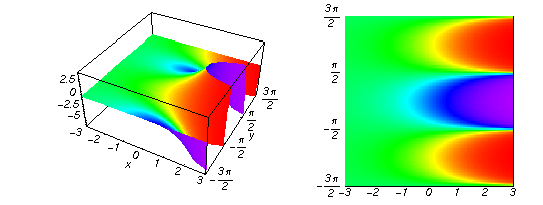
\includegraphics[width=7cm]{exp1.png} }}%
  \qquad
  \subfloat[\centering Imaginarni del]{{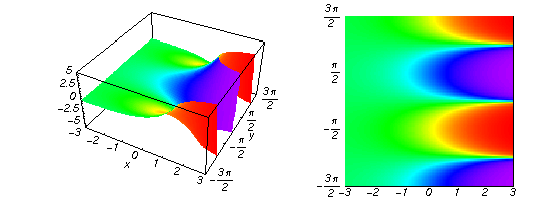
\includegraphics[width=7cm]{exp2.png} }}%
  \caption{Realni in imaginarni del sinusne funkcije v kompleksni ravnini}%
\end{figure}

\begin{opomba}
  Zadnja trditev velja po principu identičnosti, ki ga bomo dokazali kasneje. 
\end{opomba}

\subsubsection{Sinusna in kosinusna funkcija} 

Definiramo 
\begin{gather*}
  \cos z = 1 - \frac{z^2}{2} + \frac{z^4}{4!} - \dots = \sum_{n = 0}^\infty (-1)^n \frac{z^{2n}}{(2n)!},\\
  \sin z = z - \frac{z^3}{3!} + \frac{z^5}{5!} - \dots = \sum_{n = 0}^\infty (-1)^n \frac{z^{2n + 1}}{(2n + 1)!}.
\end{gather*}
Ponovno sta oba konvergenčna polmera $R = \infty$ -- to 
je dovolj preveriti za $z \in \R$, kjer lahko preprosto uporabimo kvocientni kriterij.
Očitno velja $(\sin z)' = \cos z$ in $(\cos z)' = - \sin z$.
in za $z \in \C$ je $e^{iz} = \cos z + i \sin z$.
Od tod pa sledita zvezi $\cos z = \frac{e^{iz} + e^{-iz}}{2}$ in $\sin z = \frac{e^{iz} - e^{-iz}}{2i}$.
Če vpeljemo še hiperbolični funkciji $\cosh (z) = \frac{e^z + e^{-z}}{2}$ in 
$\sinh (z) = \frac{e^z - e^{-z}}{2}$, dobimo 
\begin{align*}
  \cosh (iz) &= \cos z & \cos(iz) &= \cosh z\\
  \sinh (iz) &= i \sin z & \quad \sin(iz) &= i \sinh z.
\end{align*}
Kot bi pričakovali, sta njuna odvoda enaka $(\sinh z)' = \cosh z$ in $(\cosh z)' = \sinh z.$
Posledica tega, kar smo izpeljali, je že znana Eulerjeva formula $e^{i\pi} + 1 = 0$.

\begin{figure}[h!]%
  \centering
  \subfloat[\centering Realni del]{{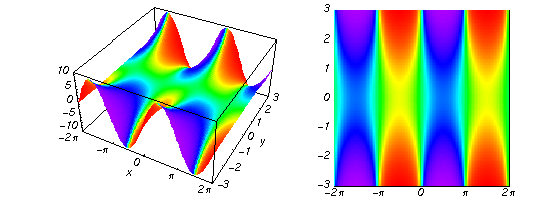
\includegraphics[width=7cm]{sin1.png} }}%
  \qquad
  \subfloat[\centering Imaginarni del]{{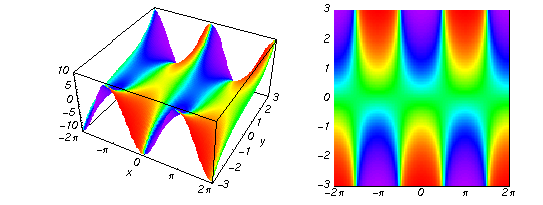
\includegraphics[width=7cm]{sin2.png} }}%
  \caption{Realni in imaginarni del eksponentne funkcije v kompleksni ravnini}%
\end{figure}

Navedimo še nekaj opazk. Za kompleksno število $z = x + yi$ 
velja zveza $e^z = e^{x + yi} = e^x (\cos y + i \sin y)$.
Torej je $|e^z| = e^{\mathrm{Re}\, z}$ in zato 
eksponentna funkcija tudi v kompleksnem nima ničel.
Hitro vidimo, da velja $e^z = 1$ natanko tedaj, ko je 
$z = 2 k \pi i$, kjer je $k \in \Z$.
Od tod pa lahko takoj vidimo, kje so ničle sinusa in kosinusa:
\begin{align*}
  \sin z = \frac{e^{iz} - e^{-iz}}{2i} = 0 &\Leftrightarrow e^{iz} = e^{-iz}\\
  &\Leftrightarrow e^{2 iz} = 1\\
  &\Leftrightarrow z = k\pi, \ k \in \Z.
\end{align*}
Podobno so ničle kosinusa oblike $z = \frac{\pi}{2} + k\pi$, kjer je $k \in \Z$.
Omenimo še, da tudi v kompleksnem veljata osnovni adicijski formuli za sinus in kosinus, in sicer 
$\cos (z + w) = \cos z \cos w - \sin z \sin w$ ter $\sin (z + w) = \sin z \cos w + \sin w \cos z$.
Iz enačbe $\cos (iy) = \frac{e^{i(iy)} + e^{-i(iy)}}{2} = \frac{e^{-y} + e^y}{2}$
pa sledi presenetljivo dejstvo, da $\cos z$ in $\sin z$ nista omejeni funkciji na $\C$.

\subsubsection{Logaritemska funkcija}

Sedaj lahko vpeljemo logaritemsko funkcijo na kompleksni ravnini.
Naj bo $w \in \C \setminus \{0\}$ in rešujemo enačbo $e^z = w$.
Naj bo $z = x + yi$ in $w = |w| (\cos \varphi + i \sin \varphi) = e^{i \arg (w)}$.
Potem je $x = \ln |w|$ in $y = \arg (w) + 2 k \pi$, kjer je $k \in \Z$.
Za $w \neq 0$ ima enačba $e^z = w$ torej neskončno rešitev:
$$z_k = \ln |w| + i \arg(w) + 2k\pi i,\ k \in \Z.$$
Logaritemska funkcija je definirana na prerezani ravnini $\C \setminus [0, \infty)$ kot 
$$w \mapsto \ln |w| + i \arg (w),\ \arg(w) \in (0, 2 \pi).$$
Ta funkcija je holomorfna na $\C \setminus [0, \infty)$, saj velja Cauchy-Riemannov sistem za realni in imaginarni del.

\begin{figure}[h!]%
  \centering
  \subfloat[\centering Realni del]{{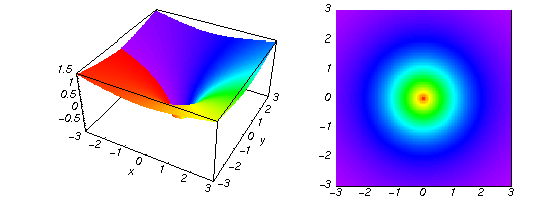
\includegraphics[width=7cm]{log1.png} }}%
  \qquad
  \subfloat[\centering Imaginarni del]{{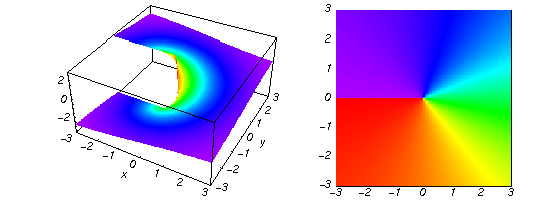
\includegraphics[width=7cm]{log2.png} }}%
  \caption{Realni in imaginarni del logaritemske funkcije v kompleksni ravnini}%
\end{figure}

\subsubsection{Korenska funkcija}

Definiramo lahko tudi potenčne funkcije na $\C$, ki jih vpeljemo kot $z \mapsto z^n$.
Za $n \in \N \cup \{0\}$ je taka funkcija holomorfna na $\C$, za $n \in \Z_-$
pa je holomorfna na $\C \setminus \{0\}$.
S tem pa naletimo na problem korena: ali obstaja tak $w$, da je $w^2 = z = |z| e^{i\arg (z)}$?
Ta enačba ima rešitvi $w = \sqrt{|z|} e^{i \frac{\arg (z)}{2}}$ in $w = \sqrt{|z|} e^{-i \frac{\arg (z)}{2}}$.
Tudi korenska funkcija ima več vej; za $\alpha \in \C$ definiramo 
$$z^\alpha = e^{a \ln (z)} = e^\alpha (\ln |z| + i \arg (z))$$
in ta funkcija je prav tako holomorfna na prerezani ravnini.

\subsection{Krivuljni integral v $\C$}

Obravnavali bomo gladke oziroma odsekoma gladke krivulje v $\C$,
ki bodo običajno usmerjene oziroma orientirane.
Gladki deli imajo regularno parametrizacijo 
$t \mapsto z(t) = x(t) + i y(t)$,
kjer je $\dot{z} (t) = \dot{x} (t) + i \dot{y} (t) \neq 0$
za vsak $t \in [a, b]$. 
Krivulja oziroma pot je sklenjena, če je $z(a) = z(b).$
Naj bo $\Gamma$ gladka krivulja v $\C$ s parametrizacijo 
$z: [a, b] \to \Gamma \subseteq \C$
in $f: \Gamma \to \C$ zvezna kompleksna funkcija.
Potem definiramo integral $f$ po $\Gamma$ kot 
\begin{align*}
  \int_\Gamma f(z)\, dz &:= \int_{\alpha} ^\beta f(z (t))\, \dot{z} (t)\, dt\\
  &= \int_a ^b f(z(t))\, (\dot{x} (t) + i \dot{y} (t))\, dt\\
  &= \int_\Gamma f(z)\, dx + i f(z)\, dy\\
\intertext{torej je to krivuljni integral forme $\omega = f\, dx + i f\, dy$
po krivulji $\Gamma$. Če pišemo $f = u + iv$, potem imamo}
  &= \int_\Gamma (u + iv)\, dx + i(u + iv)\, dy\\
  &= \int_\Gamma (u\, dx - v\, dy) + i \int_\Gamma (v\, dx + u\, dy)
\end{align*}
in vidimo, da je ta definicija neodvisna od parametrizacije krivulje 
$\Gamma$, ki ohrani njeno orientacijo.
Srečali pa bomo tudi integral oblike 
\begin{align*}
  \int_\Gamma f(z)\, d\overline{z} 
  &:= \int_a ^b f(z(t))\, (\dot{x} (t) - i \dot{y} (t))\, dt\\
  &= \int_\Gamma (u\, dx + v\, dy) + i \int_\Gamma (v\, dx - u\, dy).
\end{align*}

\begin{zgled}
  Parametriziramo rob diska $\partial \Delta (\alpha, r)$ kot $z = \alpha + r e^{it}$, kjer je 
  $t \in [0, 2\pi)$. Potem je $dz = r i e^{it}\, dt$ in izračunamo integral
  $$\int_{\partial \Delta(\alpha, r)} \frac{dz}{z - \alpha} = \int_0 ^{2\pi} \frac{r i e^{it}}{r e^{it}}\, dt = 2 \pi i.$$
\end{zgled}

\begin{zgled}
  Analogno izračunamo integral 
  \begin{align*}
    \int_{\partial \Delta (\alpha, r)} \frac{d\overline{z}}{z - \alpha} = \int_0 ^{2\pi} \frac{-r e^{-it} i}{r e^{it}}\, dt = 0.
  \end{align*}
\end{zgled}

\begin{lema}
  Imamo oceno za krivuljne integrale:
  $$\left| \int_\Gamma f(z)\, dz \right| \leq \sup_{\Gamma} |f| \cdot l(\Gamma).$$
\end{lema}

\begin{dokaz}
  Naj bo $\Gamma$ gladka in $z(t)$ njena parametrizacija za $t \in [\alpha, \beta]$.
  Tedaj je 
  \begin{align*}
    \left| \int_\Gamma f(z)\, dz \right| &= \left| \int_\alpha ^\beta f(z(t)) \dot{z}\, dt \right |\\
    &\leq \int_\alpha ^\beta |f(z(t))| |\dot{z} (t)|\, dt\\
    &\leq \sup_\Gamma |f| \int_\alpha ^\beta |\dot{z} (t)|\, dt = \sup_{\Gamma} |f| \cdot l(\Gamma). \qedhere
  \end{align*}
\end{dokaz}

\begin{trditev}
  Naj bo $D$ odprta v $\C$ in naj bo $f: D \to \C$ holomorfna z zveznim odvodom $f' \in C(D)$.
  Naj bo $\Gamma \subseteq D$ odsekoma gladka krivulja od točke $a \in D$
  do točke $b \in D$.
  Tedaj je $$\int_\Gamma f'(z)\, dz = f(b) - f(a) = \int_a ^b f'(z)\, dz.$$
\end{trditev}

\begin{opomba}
  Izkaže se, da velja tudi trditev v obratno smer; če je integral $\int_{\Gamma} f(z)\, dz$ neodvisen od poti 
  na območju $D$, ima $f$ primitivno funkcijo.
\end{opomba}

\begin{dokaz}
  Vemo, da je $d_z f = f'(z)\, dz$ in $du = u_x \, dx + u_y\, dy = \grad u \cdot d\vec{r}$.
  Torej je 
  \begin{align*}
    \int_{\Gamma} f'(z)\, dz &= \int_\Gamma df\\
    &= \int_\Gamma du + i\, dv\\
    &= \int_\Gamma \grad u\, d\vec{r} + i \int_\Gamma \grad v \, d\vec{r}\\
    &= f(b) - f(a). \qedhere
  \end{align*}
\end{dokaz}

\begin{posledica}
  Če je $n \in \N \cup \{0\}$, potem velja
  $$\int_{\partial \Delta (\alpha, r)} (z - \alpha)^n\, dz = \int_{\partial \Delta (\alpha, r)} \frac{d}{dz} \left(\frac{(z - \alpha)^{n + 1}}{n + 1}\right)\, dz = 0.$$
\end{posledica}

\begin{posledica}
  Če je $n \in \{-2, -3, \dots\}$, potem velja
  $$\int_{\partial \Delta (\alpha, r)} (z - \alpha)^n\, dz = \int_{\partial \Delta (\alpha, r)} \frac{d}{dz} \left(\frac{(z - \alpha)^{n + 1}}{n + 1}\right)\, dz = 0.$$
\end{posledica}

Od tod sledi 
$$\frac{1}{2 \pi i} \int_{\partial \Delta (\alpha, r)} (z - \alpha)^n\, dz = \begin{cases}
  0&; n \in \Z \setminus \{-1\}\\
  1&; n = -1.
\end{cases}$$

\begin{opomba}
  Funkcija $\frac{1}{z}$ torej ni odvod holomorfne
  funkcije v $\C \setminus \{0\}$.
  Možen kandidat za primitivno funkcijo bi bil logaritem,
  ki pa ni dobro definiran na $\C \setminus \{0\}$.
\end{opomba}

\begin{izrek}[Greenova formula v $\C$]
  Naj bo $D$ omejena odprta množica v $\C$ z odsekoma gladkim robom, sestavljenim iz končnega števila
  odsekoma gladkih krivulj, orientiranih pozitivno glede na $D$.
  Naj bosta $f, g \in C^1 (\overline{D})$ kompleksni funkciji. 
  Tedaj je 
  $$\int_{\partial D} f\, dz + g\, d\overline{z} = 2i \iint_D (f_{\overline{z}} - g_z)\, dx\, dy.$$
\end{izrek}

\begin{posledica}[Cauchyjev izrek]
  Naj bo $f \in \mathcal{O} (D) \cap C^1 (\overline{D})$.
  Potem je $\int_{\partial D} f(z)\, dz = 0.$
\end{posledica}

\begin{dokaz}[Dokaz izreka]
  Poračunamo 
  \begin{align*}
    \int_{\partial D} f\, dz + g\, d\overline{z} &= \int_{\partial D} f (dx + i\, dy) + g (dx - i\, dy)\\
    &= \int_{\partial D} (f + g)\, dx + i(f - g)\, dy\\
    &= \iint_D \left(i(f - g)_x - (f + g)_y\right)\, dx\, dy\\
    &= \iint_D \left((i f_x - f_y) - (i g_x + g_y)\right)\, dx\, dy\\
    &= 2i \iint_D (f_{\overline{z}} - g_{z})\, dx\, dy, 
  \end{align*}
  kjer smo upoštevali $f_{\overline{z}} = \frac{1}{2} \left(f_x + i f_y\right)$ in $g_z = \frac{1}{2} \left(g_x - i g_y\right)$.
\end{dokaz}

\begin{izrek}[Cauchyjeva formula]
  Naj bo $D$ kot v prejšnjem izreku in $f \in C^1 (\overline{D}) \cap \mathcal{O} (D)$.
  Naj bo $\alpha \in D$.
  Tedaj je 
  $$f(\alpha) = \frac{1}{2 \pi i} \int_{\partial D} \frac{f(z)}{z - \alpha}\, dz.$$
\end{izrek}

\begin{opomba}
  Cauchyjeva formula nam pove, da je holomorfna funkcija $f$ na $D$ popolnoma določena 
  s svojimi robnimi vrednostmi. Če torej "`poznamo"' holomorfna funkcijo na robu $\partial D$,
  jo poznamo na celem $D$. Funkciji $z\mapsto \frac{1}{2 \pi i} \frac{1}{z - \alpha}$
  pravimo Cauchyjevo jedro. Zgornja formula spominja na konvolucijo $\frac{1}{2 \pi i} \left(f * \frac{1}{z}\right) (\alpha)$.
\end{opomba}

\begin{dokaz}
  Naj bo $r_0 > 0$, da je $\overline{\Delta (\alpha, r_0)} \subseteq D$.
  Sedaj iz $D$ izrežemo točko $\alpha$, torej vzamemo $0 < r \leq r_0$
  in $D_r = D \setminus \overline{\Delta (\alpha, r)}$.
  Potem je $\partial D_\gamma = \partial D \cup \partial \Delta (\alpha, r)$,
  kjer je orientacija dela tega toba, ki pripada $\partial \Delta (\alpha, r)$,
  nasprotna od pozitivne orientacije $\partial \Delta (\alpha, r)$.
  Uporabimo Cauchyjev izrek za funkcijo $z \mapsto \frac{f(z)}{z - \alpha}$,
  ki je v $C^1 (\overline{D_r}) \cap \mathcal{O} (D_r)$.
  Torej imamo $\int_{\partial D_r} \frac{f(z)}{z - \alpha}\, dz = 0$ in od tod
  $$\int_{\partial D} \frac{f(z)}{z - \alpha}\, dz - \int_{\partial \Delta(\alpha, r)} \frac{f(z)}{z - \alpha}\, dz = 0.$$
  Če vpeljemo parametrizacijo $z = \alpha + re^{i \varphi}$ in dobimo 
  \begin{align*}
    \int_{\partial D} \frac{f(z)}{z - \alpha}\, dz &= \int_{\partial \Delta(\alpha, r)} \frac{f(z)}{z - \alpha}\, dz\\
    &= i \int_0 ^{2 \pi} f(\alpha + re^{i\varphi})\, d\varphi\\
    \intertext{za vsak $0 < r \leq r_0$.
  Če pošljemo $r \downarrow 0$ in upoštevamo zveznost $f$ v $a$, dobimo}
    &= i f(\alpha) \int_0 ^{2 \pi} 1\cdot d\varphi = 2 \pi i f(\alpha). \qedhere
  \end{align*}
\end{dokaz}

\begin{posledica}[Lastnost povprečne vrednosti]
  Naj bo $f \in O(D) \cap C^1 (D)$. Naj bo $\alpha \in D$, $r > 0$ 
  in $\overline{\Delta} (\alpha, r) \subseteq D$.
  Tedaj je 
  $f(\alpha) = \frac{1}{2 \pi} \int_0 ^{2 \pi} f(\alpha + re^{it})\, dt$.
\end{posledica}

\begin{dokaz}
  Uporabimo Cauchyjevo formulo za $\Delta (\alpha, r)$:
  \begin{align*}
    f(\alpha) &= \int_{\partial \Delta (\alpha, r)} \frac{f(\xi)}{\xi - a}\, d\xi\\
    &= \frac{1}{2\pi i} \int_0 ^{2\pi} \frac{f(\alpha + re^{it})}{r e^{it}}\, r \cdot i \cdot e^{it}\, dt\\
    &= \frac{1}{2 \pi} \int_0 ^{2 \pi} f(\alpha + r e^{it})\, dt,
  \end{align*}
  kjer smo vpeljali parametrizacijo $\xi = \alpha + e^{it}$ za $t \in [0, 2\pi)$
  in $d\xi = r \cdot i \cdot e^{it}\, dt.$
\end{dokaz}

\begin{trditev}
  Naj bo $D$ kot v Greenovi formuli. Naj bo $f \in \mathcal{O} (D) \cap C^1 (\overline{D})$.
  Tedaj je $f \in C^{\infty} (D)$ in za $\alpha \in D$ velja
  $$f^{(n)} (\alpha) = \frac{n!}{(2 \pi i)} \int_{\partial D} \frac{f(\xi)}{(\xi - \alpha)^{n + 1}}\, d\xi.$$ 
\end{trditev}

\begin{dokaz}
  Vemo, da je $f(\alpha) = \frac{1}{2 \pi} \int_{\partial D} \frac{f(\xi)}{\xi - \alpha}\, d\xi$.
  Potem je $f(z) = \frac{1}{2 \pi} \int_{\partial D} \frac{f(\xi)}{\xi - z}\, d\xi$
  za vsak $z \in D$. Definirajmo torej 
  $$F(z) := \frac{1}{2\pi} \int_{\partial D} \frac{f(\xi)}{\xi - z}\, d\xi.$$
  Potem je $F$ integral s parametrom $z$, ki je dobro definiran na $\C \setminus \partial D$.
  Tako je
  \begin{align*}
    \frac{\partial }{\partial z} \left(\frac{1}{2 \pi i} \int_{\partial D} \frac{f(\xi)}{\xi - z}\, d\xi\right) = \frac{1}{2 \pi i} \int_{\partial D} \frac{f(\xi)}{(\xi - z)^2}\, d\xi = F'
  \end{align*}
  zvezna na $D$ in je 
  $$\frac{\partial }{\partial \overline{z}} \left(\frac{1}{2 \pi i} \int_{\partial D} \frac{f(\xi)}{\xi - z}\, d\xi\right) = 0.$$
  Od tod sledi, da je $F \in C^1 (D)$ in $F \in \mathcal{O} (D)$.
  Po definiciji velja $F = f$ in torej 
  $$f'(z) = \frac{1}{2 \pi i} \int_{\partial D} \frac{f(\xi)}{(\xi - z)^2}\, d\xi.$$
  Desna stran je $C^\infty (D)$ in holomorfna na $D$.
  Po indukciji dobimo 
  \begin{equation*}
    f^{(n)} (z) = \frac{n!}{(2 \pi i)} \int_{\partial D} \frac{f(\xi)}{(\xi - z)^{n + 1}}\, d\xi. \qedhere
  \end{equation*}
\end{dokaz}

Sedaj smo izreke dokazali ob predpostavki, da je funkcija $f$ hkrati v $\mathcal{O}(D)$
in $C^1 (D)$. Sedaj pa bomo dokazali, da je za gladkost na $D$
druga predpostavka nepotrebna. Gladkost na $\partial D$ pa je popolnoma
 drugo vprašanje.

\begin{izrek}[Morerov izrek]
  Naj bo $f: D \to \C$ zvezna. Denimo, da je $\int_{\partial T} f(z)\, dz = 0$
  za vsak trikotnik $T \subseteq D$. Tedaj je $f \in \mathcal{O} \cap C^{\infty} (D).$
\end{izrek}

\begin{izrek}[Goursatov izrek]
  Naj bo $f \in \mathcal{O} (D)$. Tedaj je $\int_{\partial T} f(z)\, dz = 0$
  za vsak trikotnik $T \subseteq D$.
\end{izrek}

\begin{posledica}
  Če je $f \in \mathcal{O} (D)$, potem je $f \in C^\infty (D)$.
\end{posledica}

\begin{dokaz}[Morera]
  Lastnosti holomorfnosti in gladkosti sta lokalni:
  če za vsak $\Delta (\alpha, r) \subseteq D$ velja $f \in \mathcal{O} (\Delta (\alpha, r)) \cap C^\infty (\Delta (\alpha, r))$,
  potem je $f \in \mathcal{O} (D) \cap C^\infty (D)$.
  Torej je izrek dovolj dokazati za $D = \Delta (\alpha, r)$.
  Naj bo $z \in \Delta (\alpha, r)$, $h \in \C$ in $z + h \in \Delta (\alpha, r)$.
  Naj bo $T$ trikotnik z oglišči $\alpha$, $z$ in $z + h$.
  Potem je $T \subseteq \Delta (\alpha, r)$.
  Naj bo
  $$F(z) := \int_\alpha ^z f(\xi)\, d\xi = \int_{[\alpha, z]} f(\xi)\, d\xi$$
  in od tod $F(z + h) =  \int_\alpha ^{z + h} f(\xi)\, d\xi = \int_{[\alpha, z + h]} f(\xi)\, d\xi$.
  Po predpostavki vemo
  \begin{align*}
    0 &= \int_{[a, z]} f(\xi)\, d\xi + \int_{[z, w]} f(\xi)\, d\xi + \int_{[z+h, a]} f(\xi)\, d\xi\\
    &= F(z) + \int_{[z, z + h]}f(\xi)\, d\xi - F(z + h),
  \end{align*} 
  zato je
  \begin{align*}
    \frac{F(z + h) - F(z)}{h} &= \frac{1}{h} \int_{[z, z + h]} f(\xi)\, d\xi\\
    &= \frac{1}{h} \int_0 ^1 f(z + th)\cdot h\,dt\\
    &=  \int_0 ^1 f(z + th)\, dt.
  \end{align*}
  Ker je $f$ zvezna, je $F'(z) = \lim_{h \to 0} \frac{F(z + h) - F(z)}{h} = f(z)$
  in zato $F \in \mathcal{O} (D) \cap C^1 (D)$. Od tod pa po prejšnjem 
  izreku $F \in C^\infty (D)$ in vsi njeni kompleksni odvodi so holomorfni.
  Torej je res $f \in \mathcal{O}(D) \cap C^\infty (D)$.
\end{dokaz}

\begin{posledica}
  Iz Goursatovega in Morerovega izreka sledi, da za poljubno holomorfno funkcijo 
  na odprti konveksni množici $D$ obstaja njena primitivna funkcija $F \in \mathcal{O}(D)$,
  tako da je $F'(z) = f(z)$ na $D$. Primitivna funkcija je ravno $F(z) := \int_\alpha ^z f(\xi)\, d\xi$
  iz dokaza Morerovega izreka.
\end{posledica}

\begin{dokaz}[Goursat]
  Naj bo $f \in \mathcal{O} (D)$ in $T_0 \subseteq D$ trikotnik.
  Potem $T_0$ razdelimo na 4 skladne trikotnike tako, da razpolovimo njegove stranice.
  Torej je 
  $$I = \int_{\partial T_0} f(\xi)\, d\xi = \int_{\partial T_0 ^1} f(\xi)\, d\xi + \int_{\partial T_0 ^2} f(\xi)\, d\xi + \int_{\partial T_0 ^3} f(\xi)\, d\xi + \int_{\partial T_0 ^4} f(\xi)\, d\xi.$$
  Vsaj en od teh integralov je večji ali enak $\frac{I}{4}$ -- označimo ta trikotnik z $T_1$ in 
  je $\left|\int_{\partial T_1}\right| \geq \frac{I}{4}$.
  Postopek ponovimo za $T_2 \subseteq T_1 \subseteq T_0$, kjer velja 
  $$\left| \int_{\partial T_2} f(\xi)\, d\xi\right| \geq \frac{I}{4^2}.$$
  Tako dobimo zaporedje vloženih trikotnikov $T_0 \supseteq T_1 \supseteq T_2 \supseteq \dots$,
  kjer velja $\left| \int_{\partial T_n} f(\xi)\, d\xi\right| \geq \frac{I}{4^n}$,
  polmer trikotnikov gre proti $0$, $\mathrm{obseg} (T_n) = \frac{\mathrm{obseg} (T_0)}{2^n}$
  in $\bigcap_{n = 1} ^\infty T_n = \{\alpha\} \in D$.
  Vemo, da je $f$ v kompleksnem smislu odvedljiva v $\alpha \in D$, 
  torej je 
  $$f(z) = f(\alpha) + f'(\alpha) (z - \alpha) + (z - \alpha) \eta (z - \alpha),$$
  kjer je $\lim_{z \to \alpha} \eta (z - \alpha) = 0.$ Naj bo $\varepsilon > 0$.
  Potem obstaja $\delta > 0$, tako da iz $|z - \alpha| < \delta$
  sledi $|\eta (z - \alpha)| < \varepsilon$.
  Obstaja tak $n_0$, da za $n \geq n_0$ velja $T_n \subseteq \Delta (\alpha, \delta)$.
  Oglejmo si integral 
  \begin{align*}
    \left| \int_{\partial T_n} \rho (\xi)\, d\xi \right| &= \left| \int_{\partial T_n} (f(\alpha) + f'(\alpha) (\xi - \alpha) + (\xi - \alpha) \eta (\xi - \alpha))\, d\xi \right|\\
    &\leq \varepsilon \int_{\partial T_n} |\xi - \alpha|\, d\xi\\
    &\leq \varepsilon\, \mathrm{obseg} (T_n) ^2\\
    &= \frac{\varepsilon}{4^n}\, \mathrm{obseg} (T_0) ^2.
  \end{align*}
  Po drugi strani pa je ta integral večji ali enak $\frac{|I_0|}{4^n}$.
  Od tod pa sledi $$\frac{|I_0|}{4^n} \leq \frac{\varepsilon}{4^n}\, \mathrm{obseg} (T_0) ^2$$
  in posledično $|I_0| \leq \varepsilon\, \mathrm{obseg} (T_0) ^2$ za vsak $\varepsilon > 0$.
  Torej je $I_0 = 0$ in lahko uporabimo Morerov izrek.
\end{dokaz}

Če je $f \in \mathcal{O} (D)$, je torej res $f \in C(D)$, kar pomeni da so 
vsi njeni odvodi tudi holomorfni na $D$.
Nekoliko bolj previdni pa moramo biti pri gladkosti na robu odprte množice $D$.

Naj bo $f = u + iv$, kjer sta funkciji $u, v: D \to \vec{R}$.
Potem sta seveda tudi $u, v \in C^{\infty} (D)$.
Vemo, da je $u_x = v_y$ in $u_y = - v_x$.
Če prvo enačbo parcialno odvajamo po $x$, drugo pa po $y$,
dobimo $u_{xx} + u_{yy} = 0$, torej je $\triangle u = 0$
in podobno tudi $\triangle v = 0$.

\begin{trditev}
  Naj bo $f = u + iv \in \mathcal{O} (D)$, kjer sta funkciji $u, v: D \to \R$.
  Tedaj sta $u, v$ harmonični na $D$.
\end{trditev} 

\begin{definicija}
  Če je $D^{\ \text{odp}} \subseteq \C$ in sta $u, v$ harmonični na $D$,
  za kateri velja $u + iv \in \mathcal{O}(D)$, sta $u, v$ harmonični konjugirani.
\end{definicija}

Če je $u$ harmonična na $D$, ali obstaja harmonična funkcija $v$ na $D$,
da je $u + iv \in \mathcal{O}(D)$? V splošnem je odgovor ponovno odvisen od topologije.

\begin{trditev}
  Naj bo $D$ zvezdasto območje v $\C$ in $u$ harmonična na $D$.
  Potem ima $u$ harmonično konjugiranko $v$, torej harmonično funkcijo $v: D \to \R$,
  da je $u + iv \in \mathcal{O} (D)$.
\end{trditev}

\begin{opomba}
  Od tod sledi tudi, da je $u \in C^\infty (D)$.
\end{opomba}

\begin{dokaz}
  Če tak $v$ obstaja, mora veljati $u_x = v_y$ in $u_y = - v_x$.
  To pomeni, da mora imeti vektorsko polje $(-u_y, u_x)$ potencial $v$.
  Tak $v$ pa obstaja, saj je 
  \begin{equation*}
    \rot (-u_y, u_x, 0) = (0, 0, u_{xx} + u_{yy}) = \vec{0}. \qedhere
  \end{equation*}
\end{dokaz}

\begin{opomba}
  V tem dokazu je $v$ določen do konstante natančno, in sicer s predpisom 
  $$v(x, y) = \int_0 ^{(x, y)} -u_y\, dx + u_x\, dy,$$
  kjer je $D$ zvezdasta glede na $0$.
\end{opomba}

\begin{zgled}
  V splošnem konjugiranka ne obstaja.
  Oglejmo si na primer $D = \C \setminus \{0\}$
  in funkcijo $u(x, y) = \ln |z| = \frac{1}{2} \ln (x^2 + y^2)$.
  Edini kandidat za konjugiranko bi bila funkcija $\mathrm{arg} (z)$,
  ki pa ni zvezna na $\C \setminus \{0\}$.
\end{zgled}

Vemo že, da je funkcija $f: D^{\ \text{odp}} \subseteq \C \to \C$,
ki se da v okolici vsake točke razviti v potenčno vrsto, holomorfna na $D$.
Sedaj pa bomo pokazali tudi obrat te trditve.

\begin{izrek}
  Naj bo $f \in \mathcal{O} (D)$, $\alpha \in D$ in $r > 0$, tako da je 
  $\overline{\Delta} (\alpha, r) \subseteq D$. Tedaj lahko $f$ na 
  $\Delta (\alpha, r)$ razvijemo v konvergentno potenčno vrsto 
  $$f(z) = \sum_{n = 0} ^\infty a_n (z - \alpha)^n = \sum_{0} ^\infty \frac{f^{(n)} (\alpha)}{n!} (z - \alpha)^n,$$
  kjer je $a_n = \frac{1}{2 \pi i} \int_{\partial \Delta (\alpha, r)} \frac{f(\xi)}{(\xi - \alpha)^{n + 1}}\,d\xi$
\end{izrek}

\begin{opomba}
  Konvergenčni polmer $R$ je torej vsaj $d(\alpha, \partial D)$, torej 
  razdalja $\alpha$ do roba $D$.
\end{opomba}

\begin{dokaz}
  Vemo, da je za vsak $z \in \Delta (\alpha, r)$ po Cauchyjevi formuli 
  $f(z) = \frac{1}{2 \pi i} \int_{\partial \Delta(\alpha, r)} \frac{f(z)}{\xi - z}\, d\xi$.
  Podrobneje si oglejmo Cauchyjevo jedro 
  $$\frac{1}{\xi - z} = \frac{1}{(\xi - \alpha) - (z - \alpha)} = \frac{1}{\xi - \alpha} \cdot \frac{1}{1 - \frac{z - \alpha}{\xi - \alpha}}.$$
  Naj bo $z \in \overline{\Delta(\alpha, \rho)}$, kjer je $0 < \rho < r$.
  Potem je $\left| \frac{z - \alpha}{\xi - \alpha} \right| \leq \frac{\rho}{r} < 1$
  za vsak $z \in \overline{\Delta(\alpha, \rho)}$ in $\xi \in \partial \Delta(\alpha, r)$.
  To pomeni, da lahko Cauchyjevo jedro razvijemo v vrsto 
  $$\frac{1}{\xi - \alpha} \left(\sum_{0} ^\infty \left(\frac{z - \alpha}{\xi - \alpha}\right)^n\right) = \sum_0 ^\infty \frac{(z - \alpha)^n}{(\xi - \alpha)^{n + 1}},$$
  ki konvergira enakomerno na $z \in \overline{\Delta(\alpha, \rho)}$ in $\xi \in \partial \Delta (\alpha, r)$.
  Sedaj zamenjamo integrirance in vsoto ter dobimo vrsto 
  $$f(z) = \sum_0 ^\infty \left(\frac{1}{2 \pi i} \int_{\partial \Delta (\alpha, q)} \frac{f(\xi)}{(\xi - \alpha)^{n + 1}}\,d\xi\right) (z - \alpha)^n,$$
  ki konvergira enakomerno na $\overline{\Delta (\alpha, \rho)}$, $0 < \rho < r$.  
\end{dokaz}

Od tod sledi, da lahko vsako celo holomorfno funkcijo $f \in \mathcal{O} (\C)$ zapišemo kot vrsto 
$f(z) = \sum_0 ^\infty a_n z^n$, ki absolutno konvergira povsod na $\C$
in konvergira enakomerno na kompaktih.

\begin{lema}\label{lem:1}
  Naj bo $f \in \mathcal{O}(\Delta(0, R))$. Tedaj za vsak $n \in \N \cup \{0\}$
  in vsak $0 < r < R$ velja ocena 
  $$|f^{(n)} (0)| \leq \frac{n!}{r^n} \max_{|z| = r} |f|.$$
\end{lema}
\begin{opomba}
  Kasneje bomo dokazali princip maksima za holomorfne funkcije, ki nam pove, 
  da velje $\max_{|z| \leq r} |f| = \max_{|z| = r} |f|$.
\end{opomba}

\begin{dokaz}
  Vemo, da je $f^{(n)} (0) = \frac{1}{2 \pi i} n! \int_{\partial \Delta (0, r)} \frac{f(\xi)}{\xi^{n + 1}}\, d\xi$.
  Torej je 
  \begin{align*}
    |f^{(n)} (0)| &\leq \frac{1}{2 \pi} n! \int_{\partial \Delta (0, r)} \frac{|f(\xi)|}{|\xi|^{n + 1}}\, d\xi\\
    &\leq \frac{n!}{2\pi} \frac{\max_{|z| = r} |f|}{r^{n + 1}} \cdot 2\pi r\\
    &= n! \frac{\max_{|\xi| = r} |f|}{r^n}. \qedhere
  \end{align*}
\end{dokaz}

\begin{opomba}
  To je poseben primer Cauchyjevih ocen.
\end{opomba}

\begin{izrek}
  Naj bo $(f_n)_{n = 1} ^\infty$ zaporedje holomorfnih funkcij na odprti množici $D \subseteq \C$,
  ki enakomerno na kompaktih v $D$ konvergira k funkciji $f$.
  Tedaj je funkcija $f$ holomorfna na $D$ in tudi zaporedje odvodov 
  $(f'_n)_{n = 1} ^\infty$ konvergira enakomerno po kompaktih v $D$ k funkciji $f'$.
\end{izrek}

\begin{dokaz}
  Po predpostavki $(f_n)_{n = 1} ^\infty$ enakomerno konvergira k $f$ na vsakem zaprtem disku, vsebovanem v $D$.
  Od tod (kot v realnem) sledi, da je $f$ zvezna na tem disku.
  Ker je tak disk poljuben, je $f$ zvezna povsod na $D$. 
  Naj bo sedaj $T \subseteq D$ zaprt trikotnik, torej je $\partial T \subseteq D$
  komnpaktna množica. To pomeni, da $(f_n)_{n = 1} ^\infty$
  na $\partial T$ enakomerno konvergira k limitni funkciji $f$.
  Od tod pa sledi $\int_{\partial T} f(z)\, dz = \lim_{n \to \infty} \int_{\partial T} f_n (z)\, dz = 0$.
  Torej je po Morerovem izreku limitna funkcija $f$ holomorfna.

  Dokažimo še, da tudi $(f_n ')_{n = 1} ^\infty$ konvergira po kompaktih v $D$ k funkciji $f'$.
  Naj bo $K \subseteq D$ kompaktna množica. Za vsak $z \in K$ naj bo $\Delta (z, r_z)$
  odprt disk, tako da velja $\overline{\Delta (z, 2r_z)} \subseteq D$.
  Zaradi kompaktnosti lahko $K$ pokrijemo s končno mnogo izmed teh diskov.
  Definiramo torej $\widetilde{K} := \overline{\Delta (z_1, 2r_{z_1})} \cup \dots \cup \overline{\Delta (z_n, 2 r_{z_n})}$ in to 
  je kompaktna množica, vsebovana v $D$. Naj bo $r = \min \{r_{z_1}, \dots, r_{z_n}\}$.
  Tedaj za vsak $z \in K$ velja, da je $D(z, r) \subseteq \widetilde{K}$. Sedaj lemo \ref{lem:1}
  uporabimo za funkcijo $f_n - f$ na $D(z, r)$ in dobimo 
  $$|f_n'(z) - f'(z)| < \frac{1}{r} \max_{\xi \in \Delta (z, r)} \{|f_n (\xi) - f(\xi)|\} \leq \frac{1}{r} \max_{\xi \in \partial \widetilde{K}} \{|f_n (\xi) - f(\xi)|\}.$$
  Za dovolj velik $n$ je torej $f'_n - f'$ enakomerno majhno na $K$. \qedhere
\end{dokaz}

\begin{posledica}
  Po predpostavkah prejšnjega izreka za vsak $j \in \N$ tudi $f_n^{(j)}$
  konvergira proti $f^{(j)}$ enakomerno po kompaktih.
\end{posledica}

\begin{izrek}[Liouvillov izrek]
  Naj bo $f \in \mathcal{O} (\C)$ cela holomorfna funkcija,
  ki narašča kot polinom: torej obstajata $M \geq 0$ in $N \in \N \cup \{0\}$,
  da za vsak $z \in \C$ velja 
  $$|f(z)| \leq M(1 + |z|^N).$$
  Potem je $f$ polinom stopnje največ $N$. 
\end{izrek}

\begin{posledica}
  Vsaka omejena cela holomorfna funkcija je konstantna.
\end{posledica}

\begin{izrek}[Osnovni izrek algebre]
  Vsak nekonstanten polinom s kompleksnimi koeficienti ima kompleksno ničlo.
\end{izrek}

\begin{posledica}
  Polinom $p(z) = a_n z^n + \dots + a_1 z + a_0$, kjer je $a_0, a_1, \dots, a_n \in \C$,
  $a_n \neq 0$ in $n\geq 1$, ima natanko $n$ kompleksnih ničel, štetih s kratnostjo.
\end{posledica}

\begin{opomba}
  Iz Liouvillovega izreka prav tako sledi, da funkciji $\sin(z)$ in $\cos(z)$
  nista omejeni na $\C$.
\end{opomba}

\begin{dokaz}
  Naj bo $f \in \mathcal{O} (D)$, torej $f(z) = \sum_0 ^\infty a_n z^n$ s konvergenčnim
  polmerom $R = \infty$. 
  Uporabimo prejšnjo lemo, da dobimo $|f^{(n)} (0)| \leq n! \frac{\max_{|z| = r} |f|}{r^n}$.
  Vemo, da je $|f(z)| \leq M(1 + |z|^N)$ za vsak $z \in \C$.
  Potem imamo $$|f^{(n)} (0)| \leq n! \frac{M (1 + r^N)}{r^n}$$
  za vsak $r > 0$. Naj bo $n > N$. Potem je $\lim_{r \to \infty} n! \frac{M (1 + r^N)}{r^n} = 0$
  in zato $a_n = \frac{f^{(n)} (0)}{n!} = 0$. Torej je $f$ polinom stopnje največ $N$.
\end{dokaz}

\begin{dokaz}[Dokaz osnovnega izreka algebre]
  Naj bo $p(z) = a_n z^n + \dots + a_1 z + a_0$.
  Potem obstaja $R> 0$, da velja ocena $|p(z)| \geq \frac{|a_n|}{2} |z|^n$
  za $|z| \geq R$.
  Denimo, da $p$ nima ničle na $\C$.
  Potem je $f(z) = \frac{1}{p(z)}$ prav tako cela holomorfna funkcija.
  Za vsak $|z| \geq R$ velja 
  $$|f(z)| = \frac{1}{|p(z)|} \leq \frac{2}{|a_n|} \frac{1}{|z|^n} \leq \frac{2}{|a_n| R^n}.$$
  Ker je $\overline{\Delta (0, R)}$ kompakt, je tam $|f|$ omejena,
  torej obstaja $M$, da je $|f(z)| \leq M$ za vsak $|z| \leq R$.
  Torej je $|f(z)| \leq \max \left\lbrace M, \frac{2}{|a_n|R^n} \right\rbrace$
  za vsak $z \in \C.$ Zato je $f$ omejena cela funkcija in tako konstantna, to pa pomeni,
  da je tudi polinom $p$ konstanten.
\end{dokaz}

\begin{trditev}[Princip maksima]
  Naj bo $D$ območje v $\C$ in $f: D \to \C$ omejena holomorfna funkcija.
  Tedaj je ali $|f(z)| < \sup_D |f|$ za vsak $z \in D$ ali pa je $f$ konstantna funkcija.
\end{trditev}

\begin{posledica}
  Naj bo $D$ omejena odprta množica v $\C$ in $f \in \mathcal{O}(D) \cap C(\overline{D})$.
  Tedaj je $\max_{\partial D} |f| = \max_ {\overline{D}} |f|$. 
\end{posledica}

\begin{dokaz}[Dokaz posledice]
  Če je $D$ omejena, je $\overline{D}$ kompaktna, torej ima $|f|$
  maksimum na $\overline{D}$. Očitno je $\max_{\partial D} |f| \geq \max_{\overline{D}} |f|$.
  Denimo, da $|f|$ zavzame maksimum v točki $\alpha \in D$.
  Potem $\alpha$ pripada neki povezani komponenti $D$.
  Po principu maksima je $f$ konstantna na tej povezani komponenti.
  Torej zavzame $|f|$ vrednost $f_{(\alpha)}$ tudi na robu te komponente
  in torej na robu $\partial D$.
\end{dokaz}

\begin{dokaz}[Dokaz trditve]
  Spomnimo se lastnosti povprečne vrednosti $f(\alpha) = \frac{1}{2\pi} \int_0 ^{2\pi} f(\alpha + re^{i\varphi})\, d\varphi$
  in od tod sledi lastnost podpovprečne vrednosti:
  $$|f(\alpha)| \leq \frac{1}{2\pi} \int_0 ^{2\pi} |f(\alpha + re^{i \varphi})|\, d\varphi.$$
  Denimo, da $f$ po absolutni vrednosti zavzame maksimum na $D$.
  Definirajmo množico $A := \{z \in D;\ |f(z)| = \sup_D |f|\}$.
  Vemo že, da je $A$ neprazna, radi bi pa tudi dokazali,
  da je hkrati odprta in zaprta v $D$.
  Zaprtost $A$ sledi iz zveznosti funkcije $z \mapsto |f(z)|$,
  saj je $A = |f|^{-1} (\{M\})$.
  Dokažimo še odprtost; naj bo $\alpha \in A$.
  Oglejmo si njeno okolico $\overline{\Delta (\alpha, r)} \subseteq D$.
  Po lastnosti podpovprečne vrednosti velja 
  \begin{align*}
    0 &\leq \frac{1}{2\pi} \int_0 ^{2\pi} (|f(\alpha + re^{i \varphi})| - |f(\alpha)|).
  \end{align*}
  Ker pa je $|f(\alpha + re^{i \varphi})| - |f(\alpha)| \leq 0$
  in je $\theta \mapsto |f(\alpha + re^{i \theta})| - |f(\alpha)|$
  zvezna, je identična $0$.
  Od tod pa sledi $|f(\alpha)| = |f(\alpha + re^{i\varphi})|$ za vsak $\varphi \in [0, 2\pi)$
  in $r >0$, da je $\overline{\Delta(\alpha, r)} \subseteq D$.
  Torej je $|f(z)| = |f(\alpha)|$ v okolici $\alpha$ in ta okolica pripada $A$, torej 
  je $A$ res odprta v $D$.
\end{dokaz}

Naš naslednji cilj je dokaz principa identičnosti. Ta nam pove, da če se dve holomorfni 
funkciji na območju ujemata na množici, ki ima stekališče na območju, 
sta funkciji enaki.

\begin{izrek}[Princip identičnosti]
  Naj bo $D$ območje in $A \subseteq D$ s stekališčem v $D$.
  Naj bo $f \in \mathcal{O} (D)$, da je $f(\alpha)= 0$ za vsak $\alpha \in A$.
  Tedaj je $f \equiv 0$ na $D$. 
\end{izrek}

\begin{trditev}
  Naj bo $f \in \mathcal{O}(\Delta (\alpha, r))$ in naj ima $f$
  v $\alpha$ ničlo $(f(\alpha) = 0)$. Tedaj je ali $f \equiv 0$
  na $\Delta (\alpha, r)$ ali pa obstaja tako naravno število $N \in \N$
  in $g \in \mathcal{O} (\Delta (\alpha, r))$, $g(\alpha) \neq 0$,
  da je $f(z) = (z - \alpha)^N g(z)$.
\end{trditev}

\begin{dokaz}[Dokaz trditve]
  Funkcijo $f$ lahko zapišemo kot $f(z) = \sum_0 ^N a_n (z - \alpha)^n$
  na $\Delta (\alpha, r)$, kjer je $a_0 = 0$.
  Če niso vsi koeficienti $a_n$ ničelni, definiramo $N$ kot najmanjši indeks,
  da je $a_N \neq 0$.
  Potem je 
  \begin{align*}
    f(z) &= a_N (z - \alpha)^N + a_{N+1} (z - \alpha)^{N + 1} + \dots\\
    &= (z - \alpha)^N (a_N + a_{N + 1} (z - \alpha) + \dots)
  \end{align*}
  Sedaj pa definiramo $g(z) = a_N + a_{N + 1} (z - \alpha) + \dots$
  in ta vrsta ima enak konvergenčni polmer kot vrsta za $f$.
  Vidimo, da $g \in \mathcal{O} (\Delta (\alpha, r))$ in $g(\alpha) \neq 0$,
  kot smo želeli.
\end{dokaz}

\begin{posledica}
  Če sta $f, g \in \mathcal{O} (D)$, tako da velja $f = g$ na $A$,
  potem je $f \equiv g$ na $D$.
\end{posledica}

\begin{zgled}
  Naj bo $f \in \mathcal{O} (\C)$ in $f \left(\frac{1}{n}\right)$ za vsak $n \in \N$.
  Potem je $f \equiv 0$ na $\C$.
\end{zgled}

\begin{zgled}
  Naj bo $w \in \R$. Funkciji $z \mapsto e^{z + w}$ in $z \mapsto e^z \cdot e^w$
  se ujemata na $\R$, zato se ujemata tudi na $\C$. Nato pa fiksiramo še $z \in \C$ 
  in uporabimo princip identičnosti na funkcijah $w \mapsto e^{z + w}$ in $w \mapsto e^z \cdot e^w$.
  Od tod dobimo, da velja $e^{w + z} = e^w e^z$.
\end{zgled}

\begin{dokaz}[Dokaz principa identičnosti]
  Naj bo $\widetilde{A} := \{z \in D;\ f(z) = f'(z) = \dots = f^{(n)} (z) = \dots = 0\}$.
  Najprej dokažimo, da je $\widetilde{A}$ hkrati odprta in zaprta v $D$.
  Zaprtost dokažemo s tem, da je $\widetilde{A} = \cap_{n = 0} ^\infty \left(f^{(n)}\right)^{-1} (\{0\})$ presek 
  zaprtih množic, saj so $f$ in vsi njeni odvodi zvezni.
  Hkrati pa je $\widetilde{A}$ tudi odprta množica v $D$, saj če je $\alpha \in \widetilde{A}$,
  lahko funkcijo $f$ razvijemo v vrsto v okolici $\overline{\Delta(\alpha, r)} \subseteq D$ kot 
  $f(z) = \sum_0 ^\infty a_n (z - \alpha)^n$, kjer so $a_n = \frac{f^{(n)} (\alpha)}{n!}$.
  Torej je $f = 0$ na $\Delta (\alpha, r)$ in so tam tudi vsi 
  njeni odvodi enaki $0$, zato $\Delta (\alpha, r) \subseteq \widetilde{A}$
  in je $\widetilde{A}$ odprta v $D$. 
  Ker je $D$ povezana, je ali $\widetilde{A} = \emptyset$ ali pa $\widetilde{A} = D$,
  kar pomeni $f \equiv 0$ na $D$.
  Naj bo $\alpha$ stekališče $A$. Na disku $\overline{\Delta(\alpha, r)} \subseteq D$
  velja ali $f = 0$ (in zato $\alpha \in A$) ali pa $f(z) = (z - \alpha)^N g(z)$,
  kjer je $N \in \N$, $g \in \mathcal{O} (\Delta(\alpha, r))$ in $g(\alpha) \neq 0$.
  Druga možnost pa bi pomenila, da je $\alpha$ izolirana ničla za $f$ 
  in da je na $\Delta(\alpha, r)$ to edina ničla $f$ (s kratnostjo $N$).
  To pa pomeni, ne more biti stekališče množice ničel $A$.
  Torej je res $f \equiv 0$ na $\Delta (\alpha, r)$ in $\alpha \in \widetilde{A}$, 
  ki je neprazna množica. Zato je $f \equiv 0$ na $D$.
\end{dokaz}

\subsection{Izolirane singularne točke}

Naj bo $D^{\ \text{odp}} \subseteq \C$ in $\alpha \in D$.
Za odprto množico $D^* = D \setminus \{*\}$ pravimo, da je punktirana ali prebodena okolica 
točke $\alpha$. Modelni primer je prav punktiran disk
$\Delta^* (\alpha, r) = \Delta (\alpha, r) \setminus \{\alpha\}$ za $r > 0$.
Za vsako funkcijo $f \in \mathcal{O} (D^*)$ pravimo, da ima v točki $\alpha$
izolirano singularnost oziroma je $\alpha$ izolirana singularna točka za $f$.

\begin{zgled}
  Če je $f \in \mathcal{O} (D)$, potem je vsak $\alpha \in D$ izolirana ničla $f$
  in $f$ je holomorfna na $D^* = D \setminus \{\alpha\}$.
\end{zgled}

\begin{zgled}
  Oglejmo si funkcijo $f(z) = \frac{\sin z}{z} \in \mathcal{O} (\C \setminus \{0\})$.
  Zdi se, da ima $f$ v točki $0$ res singularnost,
  saj tam izraz $\frac{\sin z}{z}$ ni definiran. 
  Če pa jo razvijemo v vrsto, dobimo $f(z) = 1 - \frac{z^2}{3!} + \frac{z^4}{5!} \pm \cdots$
  za $z \neq 0$. Ta potenčna vrsta ima konvergenčni polmer enak $R = \infty$ in če definiramo 
  $f(0): = 1$, postane funkcija cela holomorfna funkcija.
  V takih primerih bomo rekli, da ima $f$ v $\alpha$ odpravljivo singularnost.
\end{zgled}

\begin{zgled}
  Oglejmo si na primer $f(z) = \frac{1}{z^5} \in \mathcal{O}(\C \setminus \{0\})$, ki ima singularnost v $\alpha = 0$.
  Tukaj pa res velja $\lim_{z \to 0} |f(z)| = \infty$ in te singularnosti se ne da odpraviti.
  Takšnim singularnosti bomo rekli pol (v tem primeru specifično pol stopnje $5$).
\end{zgled}

\begin{zgled}
  Oglejmo si še funkcijo $f(z) = e^{\frac{1}{z}} \in \mathcal{O} (\C \setminus \{0\})$, ki ima singularnost v $\alpha = 0$.
  Hitro lahko pokažemo, da v vski okolici točke $\alpha$ obstaja neskončno mnogo točk, ki zavzamejo izbrano 
  pozitivno vrednost. Vidimo torej, da je obnašanje $f$ v okolici $\alpha$ dokaj divje.
  Takšni izolirani singularni točki bomo rekli bistvena singularna točka.
\end{zgled}

Naj bo $f \in \mathcal{O} (\Delta^* (\alpha, R))$, $0 < \rho < r < R$ in
$z \in \Delta^* (\alpha, R)$, tako da velja $\rho < |z - \alpha| < r$.
Za ta kolobar uporabimo Cauchyjevo formulo
\begin{align*}
  f(z) &= \frac{1}{2 \pi i} \int_{\partial A(\alpha, \rho, r)} \frac{f(\xi)}{\xi - z}\, d\xi \\
  &= \frac{1}{2 \pi i} \int_{|\xi - \alpha| = r} \frac{f(\xi)}{\xi - z}\, d\xi - \frac{1}{2 \pi i} \int_{|\xi - \alpha| = \rho} \frac{f(\xi)}{\xi - z}\, d\xi.\\
\end{align*}
Oglejmo si kompakt $\rho < \rho' \leq |z - \alpha| \leq r' < r$.
Obravnavali bomo enakomerno konvergenco na kompaktnih podmnožicah kolobarja.
Razvijemo Cauchyjevo jedro v 
\begin{align*}
  \frac{1}{\xi - z} &= \frac{1}{(\xi - \alpha) - (z - \alpha)}\\
  &= \frac{1}{(\xi - \alpha) (1 - \frac{z - \alpha}{\xi - \alpha})}\\
  &= \sum_{n = 0} ^\infty \frac{(z - \alpha)^n}{(\xi - \alpha)^{n + 1}}
\end{align*}
in ta vrsta konvergira enakomerno za $|z - \alpha| \leq r' < r$ in $|\xi - \alpha| = r$
Torej je 
\begin{align*}
  \frac{1}{2 \pi i} \int_{|\xi - \alpha| = r} \frac{f(\xi)}{\xi - z}\, d\xi = \sum_{n = 0} ^\infty \left(\frac{1}{2 \pi i} \int_{|\xi - \alpha| = r} \frac{f(\xi)}{(\xi - \alpha)^{n + 1}}\, d\xi\right) (z - \alpha)^n.
\end{align*}
Ker sta bila $r' < r < R$ poljubna, sklepamo, da vrsta konvergira za vsak $|z - \alpha| < R$
in enakomerno na kompaktih v $\Delta(\alpha, R)$ (konvergenčni polmer je vsaj $R$).
Sedaj si oglejmo še drugi integral v Cauchyjevi formi.
Naj bo tokrat $\rho < \rho' \leq |z - \alpha|$. Potem imamo 
\begin{align*}
  -\frac{1}{\xi - z} &= -\frac{1}{(\xi - \alpha) - (z - \alpha)}\\
  &= \frac{1}{(z - \alpha) (1 - \frac{\xi - \alpha}{z - \alpha})}\\
  &= \sum_{n = 0} ^\infty \frac{(\xi - \alpha)^n}{(z - \alpha)^{n + 1}}
\end{align*}
in tokrat vrsta konvergira enakomerno za $|z - \alpha| \geq \rho' > \rho$ in $|\xi - \alpha| = \rho$.
Zato lahko ponovno vrsto nesemo v integral in dobimo 
\begin{align*}
  -\frac{1}{2 \pi i} \int_{|\xi - \alpha| = \rho} \frac{f(\xi)}{\xi - z}\, d\xi = \sum_{n = 0} ^\infty \left(\frac{1}{2 \pi i} \int_{|\xi - \alpha| = \rho} {f(\xi)}{(\xi - \alpha)^{n}}\, d\xi\right) \frac{1}{(z - \alpha)^{n+1}}.
\end{align*}
Ker sta ponovno bila $0 < \rho < \rho'$ poljubna, vrsta konvergira za vsak $z \neq \alpha$
in enakomerno na kompaktih v $\C \setminus \{\alpha\}$.
S tem smo izpeljali vrsto 
$\sum_{-\infty} ^\infty a_n (z - \alpha)^n$, kjer je $a_n = \frac{1}{2 \pi i} \int_{|\xi - \alpha| = r} \frac{f(\xi)}{(\xi - \alpha)^{n + 1}}\, d\xi$. 
Pri tem smo upoštevali, da je integral $\int_{|\xi - \alpha| = r} \frac{f(\xi)}{(\xi - \alpha)^{n + 1}}\, d\xi$ po Cauchyjevem izreku. 
neodvisen od izbire polmera $0 < r< R$.

\begin{opomba}
  V izpeljali bi lahko bil tudi $R = \infty$.
\end{opomba}

\begin{izrek}[Razvoj v Laurentovo vrsto]
  Naj bo $f \in \mathcal{O}(\Delta^* (\alpha, R))$. Potem lahko $f$ razvijemo v Laurentovo vrsto
  $f(z)= \sum _{-\infty} ^{\infty} a_n (z - \alpha)^n$,
  pri čemer je $a_n = \frac{1}{2 \pi i} \int_{|\xi - \alpha| = r} \frac{f(\xi)}{(\xi - \alpha)^{n + 1}}\, d\xi$
  Ta vrsta konvergira absolutno za vsak $z \in \Delta^* (\alpha, R)$
  in enakomerno na kompaktnih podmnožicah $\Delta^* (\alpha, R)$.
  Regularni del vrste $\sum_0 ^\infty a_n (z - \alpha)^n$ konvergira absolutno 
  za vsak $z \in \Delta(\alpha, R)$ in enakomerno na kompaktih v $\Delta(\alpha, R)$,
  glavni del vrste $\sum_{-\infty} ^{-1} a_n (z - \alpha)^n$ pa konvergira absolutno na $\C \setminus \{\alpha\}$
  in enakomerno na kompaktih v $\C \setminus \{\alpha\}$.
\end{izrek} 

\begin{definicija}
  Naj bo $f(z)= \sum_{0} ^\infty a_n (z - \alpha)^n + \sum_{-\infty} ^{-1} a_n (z - \alpha)^n$
  na $\Delta^* (\alpha, R)$.
  \begin{enumerate}
    \item $f$ ima v $\alpha$ odpravljive singularno točko, če je glavni del vrste identično enak nič. 
    \item $f$ ima v $\alpha$ pol stopnje $N \in \N$, če je $a_{-N} \neq 0$ in $a_{-N-j} = 0$ za vsak $j \in \N$.
    \item $f$ ima v $\alpha$ bistveno singularnost, če je neskončno mnogo členov glavnega dela različnih od nič.
  \end{enumerate}
\end{definicija}

\begin{zgled}
  Oglejmo si sedaj začetne primere sedaj, ko smo spoznali tipe izoliranih singularnosti.
  Funkcija $f(z) = \frac{\sin z}{z} = 1 - \frac{x^2}{3!} + \frac{z^4}{5!} \mp \dots$
  ima glavni del enak nič, zato ima v $0$ odpravljivo singularnost.
  Funkcija $\frac{1}{z^5}$ ima očitno pol stopnje $5$, funkcijo 
  $e^{\frac{1}{z}}$ pa lahko razvijemo kot 
  $$e^{\frac{1}{z}} = 1 + \frac{1}{z} + \frac{1}{2! \cdot z^2} + \dots + \frac{1}{n! \cdot z^n} + \dots$$
  in $0$ je po naši definiciji res bistvena singularna točka. 
\end{zgled}

Sedaj bomo karakterizirali tip izolirani singularne točke
glede na obnašanje funkcije v njeni okolici.

\begin{trditev}
  Naj bo $f \in \mathcal{O} (\Delta^* (\alpha, r))$. Funkcija $f$ ima v $\alpha$
  odpravljivo singularnost natanko tedaj, ko je $f$ omejena na neki njeni izbrani prebodeni okolici 
  $\alpha$; torej obstaja tak $0 < \rho < r$, da je $f$ omejena na $\Delta^* (\alpha, \rho)$.
\end{trditev}

\begin{dokaz}
  Dokažimo najprej v eno smer $(\Rightarrow)$. Naj ima $f$ v $\alpha$
  odpravljivo singularnost.
  Potem lahko zapišemo $f(z) = \sum_0 ^\infty a_n (z - \alpha)^n$ na $\Delta^* (\alpha, r)$,
  kjer je konvergenčni polmer te vrste vsaj $r$.
  Če definiramo $f(\alpha) := a_0$, je $f(z) = \sum_0 ^\infty a_n ( z - \alpha)^n$
  na $\Delta(\alpha, r)$ in je $f$ holomorfna na $\Delta (\alpha, r)$.
  Ker je torej zvezna, je omejena na vsakem disku $\Delta (\alpha, \rho) \subseteq \overline{\Delta (\alpha, \rho)}$
  za vsak $0 < \rho < r$. 
  
  Še dokaz v drugo smer $(\Leftarrow)$.
  Naj bo $f$ omejena na $\Delta (\alpha, \rho)$ za nek $0 < \rho \leq r$.
  Vemo, da za $n \in \N$  velja 
  $$a_{-n} = \frac{1}{2\pi i} \int_{\partial \Delta (\alpha, \rho')} \frac{f(\xi)}{(\xi - \alpha)^{-n +1}}\, d\xi = \frac{1}{2\pi i} \int_{\partial \Delta (\alpha, \rho')} f(\xi) (\xi - \alpha)^{n - 1}\, d\xi$$
  za vsak $0 < \rho' < \rho$. Parametriziramo krožnico $\xi = \alpha + \rho' e^{i\varphi}$, kjer teče $\varphi \in [0, 2\pi)$
  in $d\xi = \rho' i e^{i \varphi} \, d\varphi.$ Tako dobimo 
  $$a_{-n} = \frac{1}{2 \pi} \int_0 ^{2 \pi} f(\alpha + \rho' e^{i \varphi}) {\rho'}^{n - 1} e^{i(n - 1) \varphi} \rho' e^{i \varphi}\, d\varphi.$$
  Torej je $|a_{-n}| \leq \rho'^n \sup_{\Delta(\alpha, \rho)} |f|$ za vsak $0 < \rho' < \rho$.
  Če pošljemo $\rho'$ proti nič, dobimo $a_{-n} = 0$, za vsak $n \in \N$.
  Torej ima $f$ v $\alpha$ odpravljivo singularnost.
\end{dokaz}

\begin{lema}
  Naj bo $f \in \mathcal{O} (\Delta^* (\alpha, R))$. Funkcija $f$ ima v $\alpha$ pol stopnje $n$ natanko tedaj, 
  ko je $f$ oblike 
  $$f(z) = \frac{g(z)}{(z - \alpha)^n},\quad g \in \mathcal{O} (\Delta (\alpha, R)),\quad g(\alpha) \neq 0.$$
\end{lema}

\begin{dokaz}
  $(\Rightarrow)$ Naj ima $f$ v $\alpha$ pol stopnje $n$. Potem je 
  \begin{align*}
    f(z) &= \frac{a_{-N}}{(z - \alpha)^N} + \dots + a_0 + a_1 (z - \alpha) + \dots\\
    &= \frac{a_{-N} + a_{-N +1} (z - \alpha) + \dots + a_0 (z - \alpha)^N + \dots}{(z - \alpha)^N}
  \end{align*}
  in definiramo $g(z) := a_{-N} + a_{-N +1} (z - \alpha) + \dots + a_0 (z - \alpha)^N + \dots$.
  Potem velja $g \in \mathcal{O}(\Delta (\alpha, R))$ in $g(\alpha) = a_{-N} \neq 0$.
  Še v obratno smer $(\Leftarrow)$. Naj bo $f(z) = \frac{g(z)}{(z - \alpha)^N}$, kjer je 
  $g \in \mathcal{O} (\Delta (\alpha, R))$ in $g(\alpha) \neq 0$.
  Potem lahko $g$ razvijemo v vrsto 
  $g(z) = b_0 + b_1 (z - \alpha) + \dots$ in dobimo 
  $$f(z) = \frac{b_0 + b_1 (z - \alpha) + \dots}{(z -\alpha)^N}$$
  in $f$ ima pol stopnje $N$ v $\alpha$.
\end{dokaz}

\begin{izrek}
  Naj bo $f \in \mathcal{O}(\Delta^*( \alpha, R))$. Funkcija $f$ ima v $\alpha$ pol natanko tedaj, ko je 
  $\lim_{z \to \alpha} |f(z)| = + \infty.$
\end{izrek}

\begin{dokaz}
  $(\Rightarrow)$ Naj ima $f$ v $\alpha$ pol. Potem za nek $N \in \N$ velja $f(z) = \frac{g(z)}{(z - \alpha)^N}$,
  kjer je $g \in \mathcal{O} (\Delta(\alpha, R))$ in $g(\alpha) \neq 0$.
  Potem je $\lim_{z \to \infty} |f(z)| = \lim_{z \to \alpha} \frac{|g(z)|}{|z - \alpha|^N} = + \infty.$
  Še v obratno smer $(\Leftarrow)$. Naj bo $\lim_{z \to \alpha} |f(z)| = \infty$.
  Potem obstaja $0 < r' < r$, tako da je $f(z) \neq 0$ za $0 < |z - \alpha| < r'$
  Potem je $h:= \frac{1}{f} \in \mathcal{O} (\Delta^* (\alpha, r'))$. Ker je $\lim_{z \to \alpha} |h| = 0$,
  je $h$ omejena na $\Delta^* (\alpha, r')$ in ima zato $h$ odpravljivo singularnost v $\alpha$. 
  Torej lahko $h$ razširimo tako, da je $h(\alpha) = 0.$
  Potem je $h(z) = (z - \alpha)^N g(z)$, kjer je $g \in \mathcal{O} (\Delta (\alpha, r'))$ in $g(\alpha) \neq 0$.
  Ker je $g(\alpha) \neq 0$, je $g(z) \neq 0$ v okolici $\Delta (\alpha, r'')$ točke $\alpha$,
  za nek $0 < r < r' < r''$. Torej lahko zapišemo $f(z) = \left(\frac{1}{g(z)}\right) (z - \alpha)^{-N}$
  in ima $f$ v $\alpha$ pol stopnje $N$.
\end{dokaz}

\begin{izrek}
  Naj bo $f \in \mathcal{O} (\Delta^* (\alpha, R))$. Potem ima funkcija $f$ v $\alpha$ bistveno singularnost 
  natanko tedaj, ko je $0 < r_0 \leq R$, da za vsak $0 <r \leq r_0$ velja $\overline{f(\Delta^* (\alpha, r))} = \C.$
  To pomeni, da je slika $f(\Delta^* (\alpha, r))$ gosta v $\C$.
\end{izrek}

\begin{dokaz}
  $(\Rightarrow)$ Če $f$ v $\alpha$ nima bistvene singularnosti, potem slika $f(\Delta^* (\alpha, r))$ ni gosta v $\C$ za dovolj majhne $0 < r_0$.
  Res; če ima $f$ v $\alpha$ odpravljivo singularnost, je v dovolj majhnih okolicah $\alpha$ omejena.
  Če pa ima $f$ v $\alpha$ pol, potem je $\lim_{z \to \alpha} |f(z)| = \infty$, torej obstaja 
  $M$, tako da obstaja $r > 0$, da za $0 < |z - \alpha| < r$ velja $|f(z)| \geq M$.
  Slika $f(\Delta^* (\alpha, r))$ ni gosta v $\C$, ker diska $\Delta (0, M)$ ni v sliki.

  Še obrat $(\Leftarrow)$. Denimo, da za $r > 0$ slika $f(\Delta^* (\alpha, r)) \neq \emptyset$ ni gosta v $\C$.
  Potem obstaja odprta množica v $\C$, ki je ta slika ne seka. Torej obstajata $A \in \C$ in $\rho > 0$,
  tako da 
  $$f(\Delta^* (\alpha, r)) \cap \Delta(A, p) =\emptyset.$$
  Za vsak $z \in \Delta^*(\alpha, r)$ je $|f(z) - A| \geq \rho > 0$, torej je $1 \geq \frac{\rho}{|f(z) - A|}$.
  Od tod sledi, da je $h(z) = \frac{1}{f(z) - A} \in \mathcal{O}(\Delta^* (\alpha, r))$ omejena.
  Torej ima $h$ v $\alpha$ odpravljivo singularnost in se jo lahko v $\alpha$ enolično definira, da je 
  $h \in \mathcal{O} (\Delta (\alpha, r))$. Funkcija $h$ ima v $\alpha$ bodisi ničlo bodisi je nima,
  v vsakem primeru pa se jo da zapisati v obliki $h(z) = (z - \alpha)^N k(z)$,
  kjer je $k \in \mathcal{O} (\Delta (\alpha, r))$, $k(\alpha) \neq 0$ in $N \in \N \cup \{0\}$
  (če je $k(\alpha) = 0$, je $N = 0$). Zato za nek $0 < r' \leq r$ na $\Delta^* (\alpha, r')$ velja 
  $f(z) = \frac{A (z - \alpha)^N + \frac{1}{k(z)}}{(z - \alpha)^N}$.
  To pa že pomeni, da ima $f$ v $\alpha$ bodisi odpravljivo singularnost (v primeru $N = 0$)
  bodisi pol (v primeru $N > 0$).
\end{dokaz}

\begin{izrek}[Veliki Picardov izrek]
  Naj ima $f$ v $\alpha$ bistveno sungularnost.
  Tedaj za vsak dovolj majhen $0 < r$ velja, da $f$ na $\Delta^* (\alpha, r)$ zavzame vse vrednosti v $\C$
  (z izjemo morda ene) neskončno mnogokrat.
\end{izrek}

\begin{zgled}
  V primeru $f(z) = e^{\frac{1}{z}}$ je izpuščena vrednost $0$.
\end{zgled}

\begin{izrek}[Mali Picardov izrek]
  Naj bo $f$ nekonstantna cela holomorfna holomorfna funkcija.
  Tedaj $f$ zavzame vse vrednosti v $\C$ z izjemo morda ene. 
\end{izrek}

\begin{posledica}
  Če cela holomorfna funkcija izpusti dve vrednosti v $\C$, je konstantna.
\end{posledica}

\begin{dokaz}
  Točko $\infty$ obravnavamo kot izolirano singularnost. Definiramo funkcijo $g(z) = f\left(\frac{1}{z}\right)$
  na $\C \setminus \{0\}$. Funkcija $g$ ima torej v $0$ res izolirano singularnost.
  Če ima $g$ v $0$ odpravljivo singularnost, potem je na $\Delta^* (0, r)$ funkcija $g$ omejena.
  Potem obstaja $M \geq 0$, da iz $0 \leq |z| <r$ sledi $|g(z)| \leq M$. Če je $\frac{1}{r} < |N|$, potem je 
  $|f(N)| \leq M$, medtem ko je na $\overline{\Delta\left(0, \frac{1}{r}\right)}$ zvezna funkcija $f$ omejena.
  Torej je $f$ omejena na $\C$, zato je po Liouvillovem izreku konstantna, kar pa vodi 
  v protislovje s predpostavko.
  Denimo torej, da ima $g$ v $0$ pol stopnje $N \in \N$, torej $g(z) = \frac{h(z)}{z^N}$ in $h$ holomorfna na $\Delta(0, 2)$.
  Potem je $|g(z)| \leq \frac{M}{|z|^N}$ za $|z| \leq 1 $, saj je $f$ zvezna in omejena na $\overline{\Delta(0, 1 )}$.
  To pa je ekvivalentno $|f(w)| \leq M|w|^N$ za $w \geq 1$.
  Ker je zvezna, je $f$ omejena na $\overline{\Delta (0, 1)}$ z $M'$, torej obstaja $C = \max\{M, M'\} > 0$, tako da je
  $|f(w)| \leq C ( 1 + |w|^N)$ za vsak $w$.
  Torej je to polinom stopnje največ $N$ in je $f: \C \to \C$ surjektivna (osnovni izrek algebre).
  Obravnavajmo še primer, ko je $0$ bistvena singularnost za $g$;
  tedaj po velikem Picardovem izreku zavzame v $\Delta^* (0, 1)$ vse vrednosti z izjemo morda ene,
  neskončno mnogokrat. To pa pomeni, da tudi $f$ zavzame vse vrednosti razen morda ene neskončno mnogokrat. 
\end{dokaz}

\begin{zgled}
  Naj bosta $f, g \in \mathcal{O} (\C)$, tako da velja $e^f + e^g = 1$.
  Potem velja hkrati $e^g,e^f \neq 0$ in $e^f, e^g \neq 0$, torej sta $e^f$ in $e^g$ konstantni funkciji.
  To pa seveda pomeni, da sta tudi $f$ in $g$ konstantni funkciji.
\end{zgled}

\begin{opomba}
  Če je $f \in \mathcal{O} (\C \setminus \overline{\Delta(0, R)})$, lahko točko $\infty$
  obravnavamo kot izolirano singularno točko za $f$. Tip singularnosti in 
  razvoj v Laurentovo vrsto določa funkcija $g(z) = f\left(\frac{1}{z}\right)$ za $|z| < \frac{1}{|R|}$.
  Točka $0$ je izolirana singularnost za $g$. 
  \begin{enumerate}
    \item Točka $\infty$ je odpravljiva singularnost za $f$, če je $0$ odpravljiva singularnost za $g$.
    V tem primeru je $g(z) = \sum_0 ^\infty a_{n} z^n$ na $\Delta^* \left(0, \frac{1}{R}\right)$
    in zato je na prebodeni okolici točke $\infty$ funkcija $f(z) = \sum_0 ^\infty a_n \frac{1}{w^n}$.
    Od tod pa sledi tudi $f(\infty) = a_0.$
    \item Funkcija $f$ ima v $\infty$ pol stopnje $N$, če ima $g$ v $0$
    pol stopnje $N$. Oglejmo si Laurentov razvoj $g(z) = \frac{a_{-N}}{z^N} + \dots + \frac{a_{-1}}{z} + a_0 + a_1 z + \cdots$,
    kjer $a_{-N} \neq 0$.
    Torej je $$f(z) = \underbrace{a_{-N}w^N + \dots + a_{-1} w}_{\textup{glavni del}} + \underbrace{a_0 + \frac{a_1}{w} + \cdots}_{\textup{regularni del}}.$$
    \item Po podobnem razmisleku ima $f$ bistveno singularnost v $\infty$, če ima $g$ bistveno singuarnost v $0$.
    Definiramo $g(z) = \dots + \frac{a_{-N}}{z^N} + \dots + \frac{a_{-1}}{z} + a_0 + a_1 z + \dots$
    in potem je 
    $$f(z) = \underbrace{\dots + a_{-N}w^N + \dots + a_{-1} w}_{\textup{glavni del}} + \underbrace{a_0 + \frac{a_1}{w} + \cdots}_{\textup{regularni del}}.$$
  \end{enumerate}
\end{opomba}

\begin{zgled}
  Funkcija $e^w$ ima v $\infty$ bistveno singularnost.
  V splošnem velja, da če ima cela holomorfna funkcija pol v točki $\infty$, potem
  je polinom.
\end{zgled}

\begin{definicija}
  Naj bo $D^{\ \text{odp}} \subseteq \C$ in $A$ končna ali neskončna podmnožica $D$, ki nima stekališča v $D$ 
  ($A$ je diskretna podmnožica $D$). Holomorfna funkcija $f: D\setminus A \to \C$ je meromorfna na $D$,
  če ima v vsaki točki $A$ pol.
\end{definicija}

\begin{opomba}
  Tako funkcijo lahko gledamo kot preslikavo $f: D \to \C P^1$, ki vse pole slika v točko $\infty$.
  To definicijo lahko uporabimo za poljubno odprto množico v $\widehat{\C}$,
  pri čemer $f$ ni identično $\infty$ na nobeni komponanti $D$. 
\end{opomba}

\begin{opomba}
  Če je $D^{\ \text{odp}} \subseteq \C$ območje in je $f$ meromorfna na $D$, se da zapisati kot ulomek $f = \frac{g}{h}$, kjer sta $g, h \in \mathcal{O} (D)$
  ter $h \neq 0.$
  Torej na meromorfne funkcije na $D$ lahko gledamo kot polje ulomkov nad kolobarjem $\mathcal{O}(D)$.
\end{opomba}

\begin{trditev}
  Naj bo $D$ območje in $f$ meromorfna na $D$. Če $f$ ni
   identično enaka $0$ na $D$, množica njenih ničel nima stekališča v $D$.
\end{trditev}

\begin{dokaz}
  Naj bo $A \subseteq D$ diskretna množica polov za $f$.
  Množica $D \setminus A$ je prav tako odprta in povezana in $f \in \mathcal{O}(D)$.
  Po principu identičnosti množica ničel od $f$ nima stekališča na $D \setminus A$.
  Ta množica tudi nima stekališča na $A$, saj ima $f$ v vsaki točki $\alpha \in A$ pol.
  To pa pomeni, da $\lim_{z \to \alpha} |f(z)| = \infty$, od tod pa že sledi, da množica ničel $f$ nima stekališča na $D$.
\end{dokaz}

\begin{definicija}
  Če je $\alpha$ izolirana singularna točka za $f$, potem koeficient $a_{-1}$ v razvoju $f$ v Laurentovo vrsto 
imenujemo residuum ali ostanek $f$ v $\alpha$ in ga označimo z $\res{f}{\alpha}$.
\end{definicija}

Ime residuum ali ostanek izvira iz dejstva, da za vsak $\overline{\Delta(\alpha, r)} \subseteq D$
velja $\frac{1}{2 \pi i} \int_{|z - \alpha| = r} f(z)\, dz = a_{-1}$. 
Vse druge člene razvoja $f$ namreč ta integral uniči.

\begin{trditev}
  Naj ima $f$ v $\alpha$ pol stopnje $N \in \N$. Tedaj je 
  $$\res{f}{\alpha} = \frac{1}{(N - 1)!} \lim_{z \to \alpha} \frac{d^{N - 1}}{dz^{N - 1}} \left(f(z) (z - \alpha)^N\right).$$
\end{trditev}

\begin{dokaz}
  Po predpostavki je $f(z) = \frac{a_{-N}}{(z - \alpha)^N} + \dots + \frac{a_{-1}}{(z - \alpha)} + a_0 + \dots$
  Od tod naprej $(z - \alpha)^N f(z) = a_{-N} + \dots + a_{-1}(z - \alpha)^{N - 1} + a_0 (z - \alpha)^{N} + \dots$
  in nato 
  $$\frac{d^{N - 1}}{dz^{N - 1}} \left(f(z) (z - \alpha)^N\right) = (N - 1)! a_{-1} + N! a_0 (z - \alpha) + \dots$$
  in trditev hitro sledi.
\end{dokaz}

\begin{izrek}
  Naj bo $D$ omejena odprta množica v $\C$ z odsekoma gladkim robom, sestavljenim iz končnega števila 
  odsekoma gladkih sklenjenih krivulj, orientiranih pozitivno glede na $D$. Naj bodo $\alpha_1, \dots, \alpha_n \in D$
  in $f \in \mathcal{O} (D \setminus \{\alpha_1, \dots, \alpha_n\}) \cap C^1 (\overline{D} \setminus \{\alpha_1, \dots, \alpha_n\})$.
  Tedaj je $$\frac{1}{2 \pi i} \int_{\partial D} f(z)\, dz = \sum_{1} ^N \res{f}{\alpha_j}.$$
\end{izrek}

\begin{posledica}
  Naj bosta $p, q$ polinoma in naj velja $\mathrm{st}\, p + 2 \leq \mathrm{st}\, q$.
  Če $q$ nima ničel na $\R$, tedaj 
  $$\int_{-\infty} ^\infty \frac{p(x)}{q(x)}\, dx = 2 \pi i \sum_{j = 1} ^n \res{\frac{p}{q}}{\alpha_j},$$
  kjer so $\alpha_1, \dots, \alpha_n$ ničle $q$ v zgornji polravnini.
\end{posledica}

\begin{zgled}
  Vemo že, da je $\int_{-\infty} ^\infty \frac{dx}{1 + x^2} = \arctan \big|_{-\infty} ^\infty = \pi.$
  Sedaj pa uporabimo prejšnjo posledico, kjer je $p = 1$ in $q = 1 + x^2$ z ničlami $\pm i$.
  Funkcija $\frac{1}{1 + z^2}$ ima pol stopnje $1$ v točki $i$.
  Od tod dobimo 
  $$\res{\frac{1}{1 + z^2}}{i} = \lim_{z \to i} \frac{z - i}{1 + z^2} = \frac{1}{2i} = - \frac{i}{2}$$
  in posledično $\int_{-\infty} ^\infty \frac{dx}{1 + x^2} = 2 \pi i \left(-\frac{i}{2} \right) = \pi.$
\end{zgled}

\begin{zgled}
  Oglejmo si $\int_{-\infty} ^\infty \frac{dx}{1 + x^4}$.
  Ponovno zapišemo $p = 1$ in $q = 1 + x^4$ in $q$ ima ničli $\alpha_1 = e^{i\frac{\pi}{4}}$
  in $\alpha_2 = e^{i\frac{3\pi}{4}} = \alpha_1^3$ na zgornji polravnini.
  Izračunamo residuuma $$\res{f}{\alpha_1} = \lim_{z \to \alpha_1} \frac{z - \alpha_1}{1 + z^4} = \frac{1}{4 \alpha_1^3} = \frac{1}{4} \overline{\alpha_2}$$
  in $$\res{f}{\alpha_2} = \lim_{z \to \alpha_2} \frac{z - \alpha_2}{1 + z^4} = \frac{1}{4 \alpha_2 ^3} = \frac{1}{4 \alpha_1} = \frac{1}{4} \overline{\alpha_1}.$$
  Sedaj uporabimo posledico in dobimo
  $$\int_{-\infty} ^\infty \frac{dx}{1 + x^4} = \frac{2\pi i}{4} (\overline{\alpha_1} + \overline{\alpha_2}) = \frac{\pi i}{2} \cdot \frac{-2 \sqrt{2} i}{2} = \frac{\pi}{\sqrt{2}}.$$ 
\end{zgled}

\begin{dokaz}[Dokaz posledice]
  Naj bo $R > 0$ tako velik, da polkrog $D_R = \{z \in \C;\ \mathrm{im}\, z > 0,\ |z| < R\}$
  vsebuje vse ničle $q$. Po izreku je $\int_{\partial D_R} \frac{p}{q}\, dz = 2 \pi i \sum_{1} ^n \res{\frac{p}{q}}{\alpha_j}$.
  Opazimo, da je $\int_{\partial D_R} \frac{p}{q}\, dz = \int_{-R} ^R \frac{p}{q}\, dz + \int_{\partial \Gamma_R} \frac{p}{q}\, dz$,
  kjer je $\Gamma_R$ lok polkroga $D_R$. Ocenimo:
  $$\left| \int_{\Gamma_R} \frac{p(z)}{q(z)}\, dz \right| = \left| \int_{0} ^\pi \frac{p(R e^{i\varphi})}{q(R e^{i\varphi})} R i e^{i\varphi}\, d\varphi  \right| \leq R \int_{0} ^\pi \frac{|p(Re^{i\varphi})|}{|q(Re^{i\varphi})|} \stackrel{R \to \infty}{\to} 0.$$
  Od tod pa dobimo 
  \begin{equation*}
    \lim_{R \to \infty} \int_{-R} ^{R} \frac{p}{q}(x)\, dx = \int_{-\infty} ^\infty \frac{p}{q} (x)\, dx = 2 \pi i \sum_{1} ^n \res{\frac{p}{q}}{\alpha_j}. \qedhere
  \end{equation*}
\end{dokaz}

\begin{dokaz}[Dokaz izreka]
  Naj bo $r > 0$ dovolj majhen, da velja $\overline{\Delta (\alpha_j, r)} \subseteq D$ za $j = 1, \dots, n$
  in $\overline{\Delta (\alpha_j, r)} \cap \overline{\Delta (\alpha_i, r)} = \emptyset$ za $i \neq j$.
  Označimo $\widetilde{D} = D \setminus \bigcup_1 ^n \overline{\Delta (\alpha_j, r)}$ in $\partial \widetilde{D} = \partial D \cup \left(\bigcup_1 ^n \partial {\Delta (\alpha_j, r)}\right)$.
  Potem je $f \in \mathcal{O}(\widetilde{D})$ in po Cauchyjevem izreku je 
  \begin{align*}
    0 = \int_{\partial \widetilde{D}} f(z)\, dz &= \int_{\partial D} f(z)\, dz + \sum_1 ^n \int_{\partial \Delta (\alpha_j, r)} f(z)\, dz\\
    &= \int_{\partial D} f(z)\, dz - 2 \pi i \sum_1 ^n \res{f}{\alpha_j}. \qedhere
  \end{align*}
\end{dokaz}

\begin{izrek}[Princip argumenta]
  Naj bo $D$ tak kot v prejšnjem izreku in $A = \{\alpha_1, \dots, \alpha_n\} \subseteq D$.
  Naj bo $f$ meromorfna na $D$ s poli v $A$, $f \in C^1 (\overline{D} \setminus A)$ in $f \neq 0$ na $\partial D$.
  Tedaj je 
  $\frac{1}{2\pi i} \int_{\partial D} \frac{f'(z)}{f(z)}\, dz$ enaka razliki števila ničel $f$ na $D$ in števila polov $f$ na $D$,
  štetih s kratnostjo.
\end{izrek}

\begin{dokaz}
  Funkcija $\frac{f'}{f}$ je holomorna na $D$.
  Naj bo $\alpha$ ali ničla ali pol $f$, vsebovan v $D$.
  V okolici $\alpha$ lahko $f$ zapišemo v obliki $f(z) = (z - \alpha)^N g(z)$,
  kjer je $g$ holomorfna v okolici $\alpha$, $g(\alpha) \neq 0$ in $N \in \Z \setminus \{0\}.$.
  Ker je $g(\alpha) \neq 0$, je $g(z) \neq 0$ v dovolj majhni okolici $\alpha$.
  Potem je $f'(z) = N(z - \alpha)^{N - 1} g(z) + (z - \alpha)^{N} g(z)$ in $\frac{f'(z)}{f(z)} = \frac{N}{z - \alpha} + \frac{g'(z)}{g(z)}$
  ter ima v ničli ali polu $f$ pol stopnje $1$. Drugi člen je holomorfen v okolici $\alpha$.
  Imamo torej $\res{\frac{f'}{g'}}{\alpha} = N$.
  Torej je $$\frac{1}{2\pi i} \int_{\partial D} \frac{f'(z)}{f(z)}\, dz = \sum_{k = 1} ^m \res{\frac{f'}{f}}{b_k},$$
  kjer je $b_k$ ničla ali pol $f$. Ker $\frac{f'}{f}$ nima drugih singularnosti na $D$, sledi želena trditev.
\end{dokaz}

\begin{opomba}
  Možne predpostavke naslednjega izreka bi lahko bile, da je $D \subseteq \overline{D} \subseteq \subseteq \Omega$,
  kjer je $D$ omejena z "`lepim"' robom, $f$ pa je meromorfen na $\Omega$ brez ničel na $\partial D$.
  Take predpostavke bomo uporabili tudi v naslednjem izreku.
\end{opomba}

\begin{izrek}[Rouchejev izrek]
  Naj bo $\Omega$ odprta množica in $D \subseteq \overline{D} \subseteq \Omega$ odprta omejena podmnožica $\C$.
  Naj ima $D$ rob kot v prejšnjih izrekih. Naj bo $f: [0, 1]_t \times \Omega_z \to \C$
  zvezna funkcija, da je za vsak $t \in [0, 1]$ funkcija $z \mapsto f(t, z) = f_t(z)$ holomorfna na $\Omega$.
  Naj bo tudi $f_t ': [0, 1] \times \Omega \to \C$ zvezna. Denimo, da velja $f(t, z) \neq 0$
  za vsak $t \in [0, 1]$ in $z \in \partial D$.
  Tedaj imata $f(0, \cdot)$ in $f(1, \cdot)$ enako število ničel na $D$.
\end{izrek}

\begin{dokaz}
  Iz prejšnjega izreka je $F(t) = \frac{1}{2 \pi i} \int_{\partial D} \frac{f_t'(z)}{f_t(z)}\, dz$ število ničel 
  $f_t$ v $D$, štetih z večkratnostjo. Po drugi strani je integrand zvezen v $(t, z)$
  in zato je $F(t)$ zvezna na $[0, 1]$.
  Torej je $F$ zvezna funkcija na $[0, 1]$ s celoštevilskimi vrednostmi, zato je konstantna
\end{dokaz}

\begin{posledica}
  Naj bosta $D$ in $\Omega$ kot v predpostavki prejšnjega izreka in naj bosta $f, g \in \mathcal{O}(\Omega)$.
  Naj bo $|f(z)| > |g(z)|$ za vsak $z \in \partial D.$
  Tedaj imata $f$ ter $f + g$ enako število ničel na $D$, štetih s kratnostjo.
\end{posledica}

\begin{dokaz}
  Definiramo $f(t, z) := f(z) + tg(z)$, ki zaradi predpostavke zadošča pogojem 
  Rouchejevega izreka. V tem primeru je $f_1 = f + g$ in $f_0 = f$.
\end{dokaz}

\begin{zgled}
  Oglejmo si $\rho(z)  = z^5 + 5z + 1$ na disku $\Delta(0, 1)$.
  Ker na njegovem robu velja $|5z| > |z|^5 + 1 > |z^5 + 1|$,
  je število ničel $\rho$ na $\Delta(0, 1)$ enako številu ničel $5z$ na enotskem disku,
  to pa je enako $1$. Podobno pa na robu $\partial \Delta(0, 2)$ velja $|z^5| > |5z| + 1 > |5z + 1|$,
  in zato ima $z^5$ na disku $\Delta(0, 2)$ enako število ničel kot $\rho$,
  torej ima $\rho$ na tej disku vseh $5$ ničel. Zato ima na območju $1 \leq z \leq 2$
  funkcija $f$ 4 ničle.
\end{zgled}

\begin{posledica}[Princip minima]
  Naj bo $\overline{\Delta (\alpha, r)} \subseteq D^{\ \text{odp}} \subseteq \C$
  in $f \in \mathcal{O} (D)$. Naj velja $|f(\alpha)| < \min_{\partial \Delta(\alpha, r)} |f(z)|$.
  Tedaj ima $f$ v $\Delta(\alpha, r)$ ničlo.
\end{posledica}

\begin{dokaz}
  Naj bo $F(z) =f(z) - f(\alpha)$. Ker je $|f(a)| < \min_{\partial \Delta (\alpha, r)} |f|$,
  je po prejšnji posledici število ničel $f$ 
  na $\Delta(\alpha, r)$ enako številu ničel $F$ na $\Delta (\alpha, r)$, kar pa je več ali enako $1$. Torej ima $f$ na tem območju res ničlo. 
\end{dokaz}

\begin{opomba}
  Pri dokazu bi se lahko oprli tudi na princip maksima; če $f$ nima ničle, tvorimo 
  $\frac{1}{f}$ in velja $\left| \frac{1}{f(a)} \right| \leq \max_{\partial \Delta (\alpha, r)} \left| \frac{1}{f(z)} \right|$
  oziroma $\min_{\partial \Delta (\alpha, r)} |f| \leq |f(\alpha)|$.
\end{opomba}

\begin{trditev}[Obstoj logaritma]
  Naj bo $D$ zvezdasto območje, $f \in \mathcal{O} (D)$ in $f$ brez ničel na $D$.
  Potem ima $f$ na $D$ logaritem, torej obstaja funkcija $g \in \mathcal{O} (D)$,
  tako da velja $f = e^g$.
\end{trditev}

\begin{opomba}
  Trditev ne velja v splošnem. Oglejmo si na primer kolobar $\Delta (0, 2) \setminus \overline{\Delta (0, 1)}$
  in funkcijo $f(z) = z$.
  Če logaritem obstaja, potem je $f' = e^g g' = f g'$.
  Od tod pa sledi $$\int_{\gamma} \frac{f'}{f}\, dz = \int_{\gamma} g'(z)\, dz = 0.$$
  za vsako sklenjeno krivuljo $\gamma \subseteq D$.
\end{opomba}

\begin{dokaz}
  Ker je $D$ zvezdasto območje glede na $0$ (brez škode za splošnost), vpeljemo 
  $$g(z) = \int_{[0, z]} \frac{f'(\xi)}{f(\xi)}\, d\xi = \int_0 ^z \frac{f'(\xi)}{f(\xi)}\, d\xi$$
  in ta $g$ je dobro definirana na $D$.
  Ker je $\frac{f'}{f} \in \mathcal{O} (D)$, velja $\int_{\partial T} \frac{f'}{f} = 0$
  na vsakem trikotniku $T$ v $D$. Od tod pa kot v dokazu Morerovega izreka 
  sklepamo, da je $g \in \mathcal{O} (D)$ in $g' = \frac{f'}{f}$.
  Oglejmo si $F(z) = f e^{-g} \in \mathcal{O} (D)$
  in vidimo $F' = f' e^{-g} + f e^{-g} (-g') = 0$. Torej je $F = e^a$ konstantna 
  preslikava in velja $f = e^{g + a}$.  
\end{dokaz}

\subsection{Holomorfne funkcije kot preslikave iz $\C$ v $\C$}

\begin{definicija}
  Oglejmo si preslikavo iz metričnih prostorov $F: (M, d) \to (N, \rho)$.
  $F$ je odprta preslikava, če je slika vsake odprte množice v $(M, d)$
  tudi odprta množica v $(N, \rho)$.
\end{definicija}

\begin{izrek}
  Naj bo $D$ območje in $f: D \to \C$ nekonstantna holomorfna funkcija .
  Potem je $f$ odprta preslikava.
\end{izrek}

\begin{opomba}
  Če je $f$ konstantna, ni odprta. Prav tako $f$ ni odprta, če je konstantna ne neki 
  komponenti $D$.
\end{opomba}

\begin{opomba}[Princip maksima]
  Direktna posledica tega izreka je princip maksima. 
  Naj bo $D$ območje, $f \in \mathcal{O}(D)$ in naj obstaja $\alpha \in D$,
  da je $|f(\alpha)| = \sup_D |f|$.
  Torej je $f(D) \subseteq \overline{\Delta (0, |f(\alpha)|)}$ in če $f$ ni konstantna,
  je odprta. To pomeni, da je v zalogi vrednosti tudi okolica $\Delta (f(\alpha), \varepsilon)$ točke 
  $f(\alpha)$ za neki $\varepsilon > 0$. Od tod pa sledi, da bi imeli v zalogi vrednosti 
  točke, ki so po absolutni vrednosti večje od $|f(\alpha)| = \sup_D |f|$, kar pa seveda ni možno.
\end{opomba}

\begin{dokaz}
  Naj bo $\alpha \in U^{\ \text{odp}} \subseteq D$. Potem na nekem disku
  $\overline{\Delta (\alpha, r)} \subseteq U$ velja 
  $f(z) - f(\alpha) = (z - \alpha)^N g(z)$, kjer je $N \in \N$, $g$ holomorfna na $\overline{\Delta(\alpha, r)}$ 
  in $g(\alpha) \neq 0$. Potem za nek $0 < r' \leq r$ velja $g(z) \neq 0$ na $\overline{\Delta (\alpha, r')}$.
  Za $|z - \alpha| = r'$ je $|(z - \alpha)^N g(z)| \geq r'^N \min_{\partial \Delta (\alpha, r')} |g| = \mu > 0$.
  Naj bo $\omega$ tak, da je $|f(\alpha) - \omega| < \mu$.
  Torej $f(z) - \omega = f(\alpha) - \omega + (z - \alpha)^N g(z)$
  in je po Roucherju število ničel $f(z) - \omega$ na $\Delta (\alpha, r')$
  enako $N > 0$, torej je res $f \left(\Delta (\alpha, r')\right) \supset \Delta (f(\alpha), \mu)$.
\end{dokaz}

\begin{izrek}[Izrek o inverzni funkciji za holomorfne funkcije]
  Naj bo $f: D \to \C$ holomorfna, $\alpha \in D$ in $f'(\alpha) \neq 0$.
  Tedaj obstaja okolica $U \ni \alpha$ in $V \ni f(\alpha)$, da je $f: U \to V$ holomorfna bijekcija 
  in je njen inverz prav tako holomorfen.
\end{izrek}

\begin{opomba}
  Holomorfna preslikava, ki je bijekcija in ima holomorfen inverz, je biholomorfizem.
  Izkaže se, da je pogoj, da je inverz holomorfen, posledica pogojev, da je $f$ 
  holomorfna bijekcija med dvema odprtima množicama.
\end{opomba}

\begin{dokaz}
  Vemo, da je diferencial enak $d_\alpha f = f'(\alpha)\, dz$.
  Ker je $f'(\alpha) \neq 0$, je odvod $\C$- oziroma $\R$-linearen avtomorfizem 
  $\C$ oziroma $\R^2$. Torej po izreku o inverzni preslikavi obstajata odprti okolici 
  $U$ in $V$ kot trdimo, da je $f: U \to V$ difeomorfizem razreda $C^\infty$.
  Naj bo $g := f^{-1} : V \to U$ preslikava razreda $C^\infty$ in $w_0, w \in V$.
  Obstajata enolična $z_0, z \in U$, da je $g(w_0) = z_0$ in $g(w) = z$.
  Zato je 
  $$\lim_{w \to w_0} \frac{g(w) - g(w_0)}{w - w_0} = \lim_{z \to z_0} \frac{z - z_0}{f(z) - f(z_0)} = \frac{1}{f'(z_0)},$$
  pri čemer okolici po potrebi zmanjšamo, da je $f'(z_0) \neq 0$ za vsak $z_0 \in U$.
  Torej je $g \in \mathcal{O}(V)$ in $g'(f(z)) = \frac{1}{f'(z_0)}$.
\end{dokaz}

\begin{izrek}
  Naj bo $D$ območje in $f \in \mathcal{O} (D)$ nekonstantna. Naj bo $\alpha \in D$
  in $m \in \N$ red ničle $z \mapsto f(z) - f(\alpha)$.
  Potem obstaja okolica $U \subseteq D$ točke $\alpha$, $\Phi \in \mathcal{O} (D)$
  in tak $r > 0$, da je: 
  \begin{itemize}
    \item $f(z) = f(\alpha) + (\Phi(z))^m$ na $U$.
    \item $\Phi' (z) \neq 0$ na $U$ in $\Phi(\alpha) = 0$.
    \item $\Phi: U \to \Delta(0, r)$ je holomorfna bijekcija oziroma biholomorfizem.
  \end{itemize}
\end{izrek}

\begin{posledica}
  Naj bo $D^{\ \text{odp}} \subseteq \C$ in $f: D \to \C$ injektivna holomorfna preslikava.
  Potem velja $f' \neq 0$ na $D$.
\end{posledica}

\begin{dokaz}[Dokaz posledice]
  Denimo, da je $\alpha \in D$ in $f'(\alpha) = 0$.
  V okolici $\alpha$ se $f$ da zapisati kot $f(z) = f(\alpha) + \Phi(z)^m$,
  kjer je $\Phi(\alpha) = 0$, $\Phi'(z) \neq 0$ v okolici $\alpha$
  in $\Phi$ biholomorfna iz okolice $U \ni \alpha$ v $\Delta(0, r)$ za nek $r > 0$
  ter $m \in \N$. Če odvajamo, dobimo $f'(z) = m \Phi(z)^{m - 1} \Phi'(z)$ na tem območju.
  Torej je $f'(\alpha) = 0$ natanko tedaj, ko je $m \geq 2$.
  Prav tako pa je funkcija $\omega \to \omega^m$ injektivna v okolici $\Delta(0, r)$
  natanko tedaj, ko je $m= 1$. Če je torej $f'(\alpha) = 0$, potem $f$ ni injektivna 
  v okolici $\alpha$ in zato ni injektivna na $D$.
\end{dokaz}

\begin{posledica}
  Naj bo $D^{\ \text{odp}} \subseteq \C$ in $f: D \to f(D)$ injektivna holomorfna funkcija.
  Potem je $f^{-1}: f(D) \to D$ holomorfna, torej je $f$ biholomorfizem iz $D$ v $f(D)$.
\end{posledica}

\begin{dokaz}[Dokaz posledice]
  Funkcija $f: D \to f(D)$ je bijekcija in ker je $f$ injektivna, ni konstantna
  na nobeni komponenti $D$. Zato je $f(D)$ odprta podmnožica $\C$, saj je $f$ odprta 
  preslikava na vsaki komponenti $D$ in zato na $D$.
  Ker je $f$ injektivna, je $f' \neq 0$ na $D$.
  Po izreku o inverzni preslikavi je inverz $f^{-1}$ holomorfen v okolici $f(\alpha)$
  za vsak $\alpha \in D$. Torej je $f^{-1}$ holomorfna na $f(D)$ in je $f$ biholomorfna iz $D$ v $f(D)$.
\end{dokaz}

\begin{dokaz}[Dokaz izreka]
  Vemo, da je $f(z) = f(\alpha) + (z - \alpha)^m g(z)$,
  kjer je $g$ holomorfna v okolici $\alpha$, $g(\alpha) \neq 0$ in $g(z) \neq 0$ 
  v neki okolici $\alpha$. Torej ima $g$ logaritem in poljuben koren, zato obstaja holomorfna funkcija $h$
  v okolici $\alpha$, tako da $h(z) \neq 0$ in je $g(z) = h(z)^m$.
  Vstavimo v začetno enačbo in dobimo $$f(z) = f(\alpha) + (z - \alpha)^m g(z) = f(\alpha) + ((z - \alpha) h(z))^m.$$
  Nato definiramo $\Phi(z) := (z - \alpha) h(z)$ in s tem je očitno zadoščeno enačbi $f(z) = f(\alpha)+ \Phi(z)^m$
  na $\Delta(\alpha, R)$. Velja pa tudi $\Phi'(z) = h(z) + (z - \alpha) h'(z)$ in zato $\Phi'(\alpha) = h(\alpha) \neq 0$
  (sa $g(\alpha) = h(\alpha)^m \neq 0$) ter $\Phi(\alpha) = 0.$
  Torej je $\Phi$ po izreku o inverzni preslikavi lokalni biholomorfizem: obstaja okolica $\alpha \in U \subseteq \Delta (\alpha, R)$
  in $r > 0$, da je $\Phi: U \to \Delta(0, r)$ biholomorfizem.
\end{dokaz}

\subsection{Mobiusove transformacije}

\begin{definicija}
  Naj bodo $a, b, c, d \in \C$, tako da je $ad - bc \neq 0$.
  Potem je preslikava $z \mapsto \frac{az + b}{cz + d}$ Mobiusova preslikava 
  ali linearna lomljena preslikava.
\end{definicija}

\begin{opomba}
  Če je $ad - bc = 0$, je bodisi $a = b = c = d$ bodisi je vsaj eden od teh števil različen od nič.
  Naj bo to $d \neq 0$. Potem je $a = \frac{bc}{d}$ in zato je $\frac{az + b}{cz + d} = \frac{b}{d}$
  za vsak $z \neq -\frac{d}{c}$.
\end{opomba}

\begin{opomba}
  Vrednosti $a, b, c, d$ določajo linearno lomljeno preslikavo.
  Če vsakega od njih pomnožimo ali delimo z nekim neničelnim številom, dobimo isto preslikavo.
  Tako lahko predpostavimo, da je $ad - bc = 1$.
\end{opomba}

Naj bo $\varphi(z) = \frac{az + b}{cz + d}$, kjer je $ad - bc \neq 0$.
Potem je $\varphi: \C P^1 \to \C P^1$ meromorfna funkcija na $\C P^1$, kjer je $\varphi\left(-\frac{d}{c}\right) = \infty$
in $\varphi(\infty) = \frac{a}{c}$. Če je $c = 0$, potem je $\varphi(z) = \frac{a}{d}z + \frac{c}{d}$ afina preslikava
in $\varphi(\infty) = \infty$ (pri tem mora seveda veljati $a \neq 0$).
Hitro vidimo, da je $\varphi: \C P^1 \to \C P^1$ bijekcija z inverzom $\varphi^{-1} (z) = \frac{dw - b}{-cw + a}$.

\begin{opomba}
  Pri inverzu lahko opazimo podobnost z matrikami. Če preslikavi 
  $\varphi(z) = \frac{az + b}{cz + d}$ priredimo matriko 
  $$A = \begin{bmatrix}
    a & b\\
    c & d
  \end{bmatrix},$$
  potem je njen inverz 
  $$A^{-1} = \begin{bmatrix}
    d & - b\\
    -c & a
  \end{bmatrix},$$
  kar ustreza $\varphi^{-1}$.
  Podobno se lahko pokaže za kompozitume Mobiusovih funkcij, ki ustrezajo množenju matrik.
\end{opomba}

Nekateri posebni primeri tega razreda preslikav so:
\begin{itemize}
  \item $z \mapsto az$, ki ustreza rotaciji za $\mathrm{arg}(a)$ in raztega za $|a|$ 
(tukaj seveda predpostavimo $a \neq 0$).
  \item $z \mapsto z + b$, ki ustreza translaciji za $b$.
  \item $z \mapsto\frac{1}{z}$, kar je inverzija na krožnico $\partial \Delta (0, 1)$.
\end{itemize}

\begin{trditev}
  Vsaka lomljena linearna preslikava je kompozitum preslikav teh treh tipov.
\end{trditev}

\begin{opomba}
  Mobiusove transformacije tvorijo grupo za kompozitum. Ta trditev nam pravi, 
  da so zgoraj naštete preslikave generatorji te grupe.
\end{opomba}

\begin{dokaz}
  Trivialen (DOPOLNI).
\end{dokaz} 

\begin{trditev}
  Lomljene linearne transformacije slikajo krožnice in premice v $\C$ v krožnice in premice v $\C$.
\end{trditev}

\begin{opomba}
  Krožnice se lahko slikao v premice, te pa v krožnice. Hitro lahko vidimo,
  da $\varphi$ slika krožnico $K$ v premico, če ima pol na $K$, in premico $p$ v premico, če 
  ima na $p$ pol (lahko tudi v točki $\infty$). Torej premico $p$ slika v krožnico,
  če tudi v $\infty$ nima pola na $p$. V ozadju je geometrijska predstava, da lahko 
  na Riemannovi sferi premice gledamo kot sfere skozi točko $\infty$.
\end{opomba}

\begin{dokaz}
  Naj bo $\partial \Delta (\alpha, r)$ krožnica s središčem v $\alpha$ in polmerom $r > 0$.
  DOPOLNI
\end{dokaz}

\begin{trditev}
  Naj bodo $\alpha, \beta, \gamma$ tri različne točke $\C P^1$. Tedaj obstaja Mobiusova transformacija $\varphi$,
  da je $\varphi(\alpha) = 0$, $\varphi(\beta) = 1$ in $\varphi(\gamma) = \infty$.
\end{trditev}

\begin{dokaz}
  Iskana Mobiusova transformacija je $\varphi(z) = \frac{(\beta - \gamma) (z - \alpha)}{(\beta - \alpha)(z - \gamma)}$.
  Če je $\gamma = \infty$, potem je $\varphi(z) = \frac{z - \alpha}{\beta - \alpha}$,
  če je $\beta = \infty$, je $\varphi(z) = \frac{z - \alpha}{z - \gamma}$ in če je 
  $\alpha = \infty$, je $\varphi(z) = \frac{\beta - \gamma}{z - \gamma}.$
\end{dokaz}

\begin{zgled}
  Naj bo $\varphi(z) = \frac{z + 1}{z - 1}$. Oglejmo si sliko roba enotskega diska 
  $\varphi(\partial \Delta)$. Ker ima $\varphi$ pol na $\partial \Delta$, je to premica.
  Ta je določena s točkama $\varphi(-1) = 0$ in $\varphi(i) = \frac{i + 1}{i - 1} = \frac{-(i + 1)^2}{2} = -i$.
  Torej je $\varphi(\partial \Delta)$ imaginarna os. Ker je $\varphi (0) = -1$, $\varphi$ slika $\Delta$
  v levo polravnino in $\C \setminus \overline{\Delta}$ v desno polravnino 
  ($\varphi$ je namreč difeomorfizem Riemannove sfere).
\end{zgled}

\subsection{Konformne preslikave}

Preslikava med dvema metričnima prostoroma je izometrija, če ohranja metriko;
to pomeni, da za $f: (D, \rho) \to (\Omega, d)$ velja $d(f(z), f(w)) = \rho(z, w)$ za vsaka $z, w \in D$.
V primeru prostorov $\R^n$ imamo standardno metriko $d(z, w) = |z - w|$,
torej za izometrije velja $|f(z) - f(w)| = |z - w|$ za vsak par $z, w$.
Sedaj izberimo $\alpha$ in opazujmo preslikavo $z \mapsto f(z + \alpha) - f(\alpha)$.
To je tudi izometrija, ki slika $0$ v $0$. Tedaj iz pogoja za izometrijo sledi 
$|f(z)| = |z|$ za vsak $z$, torej $f$ ohranja normo. Skupaj pa nam ta dva pogoja dasta,
da $f$ ohranja skalarni produkt, torej velja $\sprod{z}{w} = \sprod{f(z)}{f(w)}$ za vsaka $z, w$.
To pa med drugim pomeni, da $f$ ohranja kote.

\begin{opomba}
  Izometrij $\R^2$ ni veliko; to so kompozitumi translacij in izometrij,
  ki slikajo izhodišče nazaj v izhodišče. SLednje pa so $\R$-linearne preslikave,
  ki jih predstavimo z ortogonalno matriko $U$, za katero seveda velja $U U^{\top} = I$.
  Takim matrikam pa ustrezajo rotacije za nek kot in zrcaljenje čez premico skozi izhodišče.
\end{opomba}

V tem razdelku se bomo omejili na preslikave, ki ohranjajo kote in orientacijo.

\begin{definicija}
  Naj bo $D^{\ \text{odp}} \subseteq \C$, $\alpha \in D$ in $f: D \to \C$ funkcija.
  Rečemo, da $f$ ohranja kote v točki $\alpha$, če obstaja tak $\varphi \in [0, 2 \pi)$,
  da je 
  $$\lim_{r \downarrow 0} \frac{f(\alpha + r e^{i\theta}) - f(\alpha)}{|f(\alpha + r e^{i\theta}) - f(\alpha)|} = e^{i \varphi} \cdot e^{i \theta}$$
  za vsak kot $\theta$.
  Če $f$ ohranja kote v vsaki točki $\alpha \in D$, je $f$ konformna na $D$.
\end{definicija}

\begin{opomba}
  Naj bo $\alpha = f(\alpha) = 0$. Potem v okolici izhodišča funkcija $f$ deluje kot razteg
  in rotacija za kot $\varphi$; po definiciji namreč velja $f(r e^{i\theta}) \approx |f(r e^{i\theta})| \cdot e^{i\theta} \cdot e^{i \varphi}$. 
\end{opomba}

\begin{opomba}
  Preslikava $z \mapsto z^n$ za $n \geq 2$ ni konformna v $\alpha = 0$,
  saj se koti v izhodišču ne ohranjajo.
\end{opomba}

\begin{figure}
  \centering
  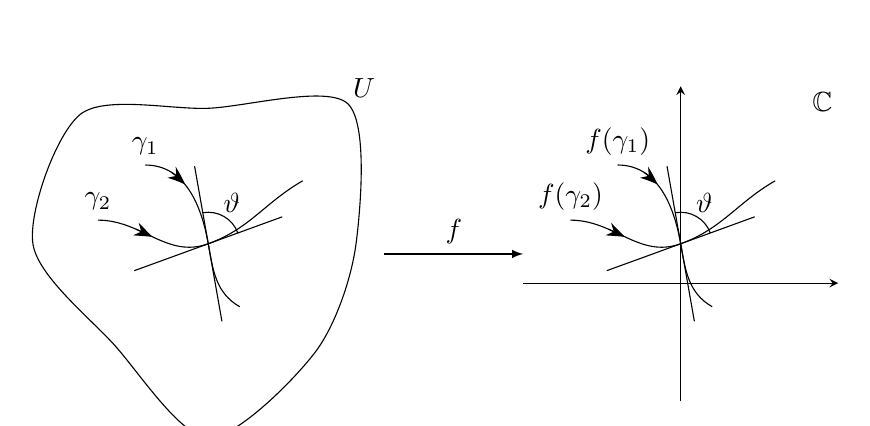
\begin{tikzpicture}[declare function={rr=2*(1+0.2*sin(3*\t-20)+0.1*rnd);}]
    \begin{scope}[local bounding box=L]
     \pgfmathsetseed{42}
     \draw plot[smooth cycle,variable=\t,samples at={0,45,...,315}] (\t:rr);
     \path (45:2.8) node{$U$};
     \draw[arr=0.25] (-0.8,1) node[above] {$\gamma_1$} to[out=0,in=100] (0,0) to[out=-80,in=150] (0.4,-0.8);
     \draw[arr=0.25] (-1.4,0.3) node[above] {$\gamma_2$} to[out=0,in=-160] (0,0) to[out=20,in=-150] (1.2,0.8);
     \draw (100:1) -- (100:-1) (20:1) -- (20:-1) (20:0.4) arc(20:100:0.4)
      (60:0.6) node{$\vartheta$};
    \end{scope}
    %
    \begin{scope}[xshift=6cm,local bounding box=R]
     \draw[arr=0.25] (-0.8,1) node[above] {$f(\gamma_1)$} to[out=0,in=100] (0,0) to[out=-80,in=150] (0.4,-0.8);
     \draw[arr=0.25] (-1.4,0.3) node[above] {$f(\gamma_2)$} to[out=0,in=-160] (0,0) to[out=20,in=-150] (1.2,0.8);
     \draw (100:1) -- (100:-1) (20:1) -- (20:-1) (20:0.4) arc(20:100:0.4)
      (60:0.6) node{$\vartheta$};
     \draw[-stealth] (0,-2) -- (0,2); 
     \draw[-stealth] (-2,-0.5) -- (2,-0.5); 
     \path (1.8,1.8) node{$\mathbb{C}$};
    \end{scope}
    %
    \draw[-latex] (L.east) -- (L.east-|R.west) node[midway,above]{$f$};
   \end{tikzpicture}
   \caption{Ohranjanje kotov pri konformni preslikavi.}
\end{figure}

\begin{izrek}
  Naj bo $D^{\ \text{odp}} \subseteq \C$ in $f: D \to \C$.
  \begin{itemize}
    \item Če je $f \in \mathcal{O} (D)$ in $f' \neq 0$ na $D$, je $f$ konformna na $D$.
    \item Če je $f$ diferenciabilna na $D$ in konformna na $D$, je $f \in \mathcal{O} (D)$
    in $f' \neq 0$ na $D$.
  \end{itemize}
\end{izrek}

\begin{dokaz}
  Dokažimo najprej prvo točko. Naj bo $\alpha \in D$.
  Potem je $f(\alpha + re^{i \theta}) - f(\alpha) = f'(\alpha) re^{i\theta} + o(r)$, torej je 
  $$\lim_{r \downarrow 0} \frac{f(\alpha + re^{i\theta}) - f(\alpha)}{|f(\alpha + re^{i\theta}) - f(\alpha)|} = \lim_{r \downarrow 0} \frac{f'(\alpha) e^{i \theta} + \frac{o(r)}{r}}{|f'(\alpha) e^{i \theta} + \frac{o(r)}{r}|} = \frac{f'(\alpha)}{|f'(\alpha)|} e^{i\theta}.$$
  Torej je $\varphi = \mathrm{arg}(f'(\alpha))$, $\frac{f'(\alpha)}{|f'(\alpha)|} = e^{i \varphi}$ in $f$ je konformna na $D$.
  Še druga točka. Naj bo $\alpha \in D$.
  Vemo, da je 
  $$f(\alpha + re^{i \theta}) - f(\alpha) = f_z (\alpha) re^{i \theta} + f_{\overline{z}} (\alpha) re^{-i\theta} + o(r).$$
  Če je $d_\alpha f = 0$, je seveda tudi $f_{\overline{z}} (\alpha) = 0$.
  Če pa je $d_\alpha f \neq 0$, ima največ 1-dimenzionalno jedro,
  saj je preslikava iz $\R^2$ nazaj vase in obstajata največ dve vrednosti $\theta \in \{ \theta_0, \theta_0+ \pi \}$, da je 
  $(d_\alpha f)e^{i \theta} = 0$. Naj bo $\theta \notin \{\theta_0, \theta_0 + \pi\}$.
  Tedaj dobimo 
  $$\lim_{r \downarrow 0} \frac{f(\alpha + r e^{i \theta}) - f(\alpha)}{|f(\alpha + r e^{i \theta}) - f(\alpha)|} = \frac{f_z (\alpha) e^{i \theta} + f_{\overline{z}} (\alpha) e^{-i\theta}}{|f_z (\alpha) e^{i \theta} + f_{\overline{z}} (\alpha) e^{-i\theta}|} = e^{i\varphi} e^{i\theta}.$$
  Od tod sledi 
  \begin{align*}
    f_z (\alpha)^2 e^{2i \theta} + f_z (\alpha) f_{\overline{z}} (\alpha) + f_{\overline{z}} (\alpha)^2 e^{-2 i \theta} &= |f_z|^2 e^{2 i \varphi} e^{2 i \theta} + f_z (\alpha) \overline{f_{\overline{z}}(\alpha)} e^{2 i \varphi} e^{4i\theta}\\
    &+ f_{\overline{z}} (\alpha) \overline{f_z (\alpha)} e^{2 i \varphi} + |f_{\overline{z}}|^2 e^{2 i \varphi} e^{2 i \theta}.
  \end{align*}
  Na to pa lahko gledamo kot enakost dveh Fourierovih vrst, zato morajo biti enaki koeficienti pri istležnh členih.
  Od tod pa sledi $f_{\overline{z}} (\alpha) = 0$, saj na desni ni členov $e^{-2 i \theta}$.
  Skupaj s prvo točko to že pomeni, da je $f \in \mathcal{O} (D)$.
  Če bi obstajal tak $\alpha \in D$, da je $f'(\alpha) = 0$, potem bi v okolici $\alpha$
  imeli $f(z) = f(\alpha) + (z - \alpha)^m h(z)$, kjer je $h \in \mathcal{O} (\Delta (\alpha, r))$,
  $h(\alpha) \neq 0$ in $m \geq 2.$ Torej je 
  $$\lim_{r \downarrow 0} \frac{f(\alpha + r e^{i \theta}) - f(\alpha)}{|f(\alpha + r e^{i \theta}) - f(\alpha)|} = e^{i m \theta} \frac{h(\alpha)}{|h(\alpha)|},$$
  s čimer smo pokazali, da $f$ ne ohranja kotov v točki $\alpha$.
\end{dokaz}

\begin{definicija}
  Območji $D$ in $\Omega$ v $\C$ sta konformno ekvivalentni,
  če obstaja biholomorfna preslikava $F: D \to \Omega$.
\end{definicija}

Konformna ekvivalenca je ekvivalenčna relacija na kompleksnih podmnožicah in če sta $D$ in $\Omega$
konformno ekvivalentni, potem sta tudi homeomorfni.
Obrat te trditve pa ne velja.

\begin{izrek}[Riemannov upodobitveni izrek]
  Naj bo $D$ enostavno povezano območje v $\C$, ki ni $\C$.
  Tedaj je $D$ konformno ekvivalenten disku $\Delta$, torej obstaja biholomorfizem 
  $f: D \to \Delta$.
\end{izrek}

Enostavno povezano območje je tako, ki "`nima lukenj"'.
To pomeni, da lahko vsako zanko stisnemo oziroma zvezno deformiramo v točko.
Če je območje $D$ zvezdasto, je seveda tudi enostavno povezano.

\begin{opomba}
  $\C$ je enostavno povezano območje, a izrek zanj ne velja, saj bi po Liouvillovem 
  izreku holomorfna funkcija $f: \C \to \Delta$ bila konstantna. Torej $\C$ in $\Delta$
  nista konformno ekvivalentni, kljub temu da sta homeomorfni.
  Tudi Riemannova sfera $\C P^1$ je enostavno povezano območje, vendar pa sploh ni homeomorfno $\C$ in $\Delta$,
  saj je kompakt.  
\end{opomba}

\begin{zgled}
  Vemo že, da preslikava $f: \Delta \to \C$ s predpisom $f(z) = \frac{z + 1}{z - 1}$
  preslika enotski disk v levo polravnino $\C$. Če to preslikavo komponiramo še z rotacijo, dobimo 
  biholomorfizem iz $\Delta$ v zgornjo polravnino $H = \{z \in \C;\ \mathrm{im}\, z > 0\}$, podan s predpisom $z \mapsto -i\frac{z+1}{z - 1}$.
  Njegov inverz iz $H$ nazaj v $\Delta$ je $z \mapsto \frac{iz + 1}{iz - 1}$
\end{zgled}

\begin{zgled}
  Območje $D = \{z \in \C;\ \arg (z) < \frac{\pi}{k}\}$ za $k \in (0, 1)$
  lahko konformno preslikamo v zgornjo polravnino z biholomorfizmom $z \mapsto z^k$.
\end{zgled}

\begin{zgled}
  Pas $\{z \in \C;\ 0 < |z| < \pi\}$ lahko konformno preslikamo v zgornjo polravnino s preslikavo $z \mapsto e^z$.
\end{zgled}

\begin{zgled}
  Dva kolobarja v $\C$ sta konformno ekvivalentna natanko tedaj, ko sta razmerji njunih premerov enaki.
\end{zgled}

\begin{figure}

  \centering
  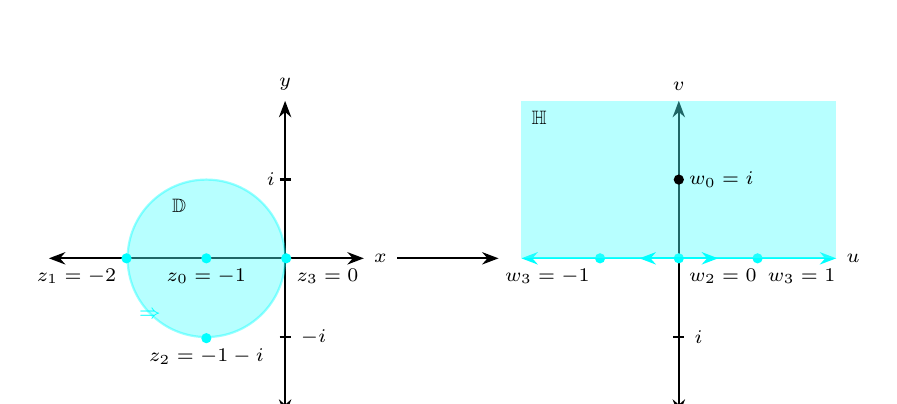
\begin{tikzpicture}[
    thick, font = \scriptsize, >={[scale =0.9]Stealth},
    fip/.style ={circle, fill = fcolor, draw = fcolor, inner sep = 1pt}
    ]


\def\OP{.4} % Deines the Opacity    
\def\GL{3}  % Defines the grid limit
\def\Fi{70} % Deines the filling percentage in contrast to the drawing
\def \yaxis{2}
    \draw [<->](-3, 0) -- (1, 0)  node (from)[anchor = west]{$x$};
    \draw [<->] (0, -\yaxis) -- (0, \yaxis) node [anchor = south]{$y$};
    \draw [->](from) --++(0:1.5)node [anchor = south, midway]{};
    \draw (-2pt, 1) -- (2pt, 1)   node    [anchor = east, left = 2pt]{$i$};
    \draw (-2pt, -1) -- (2pt, -1) node    [anchor = west]            {$-i$};

    \node (CI) at (-{\yaxis/2}, 0) [fip, fill = fcolor!\Fi, opacity = \OP, minimum size = \yaxis cm]{};
    \node at (CI.west)     [anchor = north east]   {$z_1 = -2$};
    \node at (CI.center)   [anchor = north]        {$z_0 = -1$};
    \node at (CI.east)     [anchor = north west]   {$z_3 = 0$};
    \node at (CI.south)    [anchor = north]        {$z_2 = -1 -i$};
    \node at (CI.110)   [anchor = north east, below = 2pt]{$\mathbb{D}$};

    \foreach \x/\y in {west, center, east, south}{
        \node [fip] at (CI.\x){};
        };
    \node at (CI.225)[color = fcolor]{$\Rightarrow$};

\begin{scope}[xshift = 5cm]
    \draw [<->, color = fcolor](-\yaxis, 0) -- (\yaxis, 0)  node [anchor = west,text = black]{$u$};
    \draw [<->] (0, -\yaxis) -- (0, \yaxis)                 node [anchor = south]            {$v$};

    \node at (0,0)  [anchor = north west]{$w_2 = 0$};
    \node at (1,0)  [anchor = north west]{$w_3 = 1$};
    \node at (-1,0) [anchor = north east]{$w_3 = -1$};
    \foreach \x in {-1, 0, 1}{
        \node at (\x, 0) [fip]{};
        }

    \fill [fill = fcolor!\Fi, opacity = \OP](-2, 0) rectangle (2, 2);
    \draw (0, 1) node [fip, fill = black, draw = black]{} node [anchor = west]{$w_0 = i$};
    \node at (-2, 2) [anchor = north west]{$\mathbb{H}$};
    \draw (-2pt, -1) -- (2pt, -1) node[anchor = west]{$i$};
    \draw [ color = fcolor, <->](-.5, 0) -- (.5, 0);
\end{scope}
    \end{tikzpicture}
    \caption{Slika konformne preslikave $z \mapsto \frac{(1-i) z + 2}{(1 + i) z + 2}$}
\end{figure}

Biholomorfni preslikavi $f: \Delta \to \Delta$ pravimo holomorfni avtomorfizem $\Delta$.
Ogledali si bomo si bomo množice avtomorfizmov $\mathrm{Aut}(\C)$, $\mathrm{Aut}(\C P^1)$ in $\mathrm{Aut} (\C P^{1})$,
ki so seveda grupe za kompozitum. 

Takoj lahko opazimo, da so funkcije oblike $f(z) = az + b,\ a\neq 0$ vsebovane v 
$\mathrm{Aut}(\C)$. Ali so to tudi vse?

\begin{trditev}
  Grupa evtomorfizmov $\C$ je podana kot $\mathrm{Aut} (\C) = \{az + b ;\ a, b \in \C,\ a \neq 0\}$.
\end{trditev}

\begin{dokaz}
  Takoj lahko predpostavimo, da je $f(0) = 0$ in $f(1) = 1$,
  saj bi sicer lahko nastavili $z \mapsto \frac{f(z) - f(0)}{f(1) - f(0)}$.
  Očitno je $\infty$ izolirana singularnost za $f$. Če bi bila bistvena singularnost,
  bi bila $f$ omejena in zato konstantna, kar bi bilo protislovje.
  Če je pol, potem je $f$ polinom in posledično tudi $f'$ polinom, ki pa nima ničle.
  Torej je $f'$ neničelna konstanta in zato $f(z) = z.$
  Za primer, ko je $\infty$ bistvena singularnost, bi lahko uporabili kar Picardov izrek.
  Ker je $f$ injektivna, mora veljati $f(\C \setminus \Delta) \cap f(\Delta) = \emptyset$.
  Ker je $\infty$ bistvena singularnost, je $f(\C \setminus \Delta)$ gosta v $\C$ in se zato seka 
  z odprto množico $f(\Delta)$, kar pa vodi v protislovje.
\end{dokaz}

\begin{trditev}
  Grupa avtomorfizmov Riemannove sfere je 
  $$\mathrm{Aut} (\C P^1) = \left\lbrace \frac{\alpha z + \beta}{\gamma z + \delta};\ \alpha,\beta, \gamma,\delta \in \C,\ \alpha \delta - \beta \gamma = 1 \right\rbrace.$$
\end{trditev}

\begin{dokaz}
  Naj bo $f: \C P^1 \to \C P^1$ biholomorfna funkcija.
  Naj bo $f(0) = a$, $f(1) = b$ in $f(\infty) = c$, kjer so $a, b, c$ paroma različni.
  Potem obstaja Mobiusova transformacija $\psi$, tako da je $\psi (a) = 0$, $\psi (b) = 1$ in $\psi (c) = \infty$.
  Sedaj definiramo $g := \psi \circ f \in \mathrm{Aut} (\C)$ in velja 
  $g(0) = 0$, $g(1) = 1$ in $g(\infty) = \infty$.
  Zaradi injektivnosti ima $g$ edini pol v $\infty$.
  Torej je $g \big| _{\C}: \C \to \C$ bijektivna in iz $g(0) = 0$ ter $g(1) = 1$ sledi $g = id$.
  Torej je res $f = \psi^{-1}$, kjer je $\psi$ Mobiusova transformacija. 
\end{dokaz}

\begin{izrek}[Schwartzova lema]
  Naj bo $f \in \mathcal{O} (\Delta)$, za katero velja 
  $f (\Delta) \subseteq \overline{\Delta}$ in $f(0) = 0$.
  Potem velja $|f(z)| \leq z$ za $\forall z \in \Delta$ in $|f'(0)| \leq 1$.
\end{izrek}

\begin{opomba}
  Dodatek k temu izreku je, da če velja $|f'(0)| = 1$ ali pa $|f(z)| = z$ za nek $z \in \Delta$,
  potem obstaja tak $\alpha \in \partial \Delta$, da je $f(z) = \alpha \cdot z$. 
\end{opomba}

\begin{dokaz}
  Definirajmo $g(z) := \frac{f(z)}{z}$ za $z \in \Delta^* = \Delta \setminus \{0\}$.
  Potem je $0$ izolirana singularna točka za $g$ in velja 
  $$\lim_{z \to 0} g(z) = \lim_{z \to 0} \frac{f(z)}{z} = \lim_{z \to 0} \frac{f(z) - f(0)}{z - 0} = f'(0).$$
  Za vsak $z \in \Delta$ je $|f(z)| \leq 1$. Naj bo $0 < r < 1$
  in potem je $|g(z)| = \frac{|f(z)|}{|z|} \leq \frac{1}{r}$ na $\overline{\Delta(0, r)}$.
  Torej je po principu maksima $|g(z)| \leq 1$ za $\forall z \in \Delta$ in od tod sledi 
  $|f(z)| \leq |z|$ in $|f'(0)| \leq 1$. Sedaj pokažimo še dodatek; če veljajo njegove predpostavke,
  potem je $|g(z_0)| = 1$ za nek $z_0 \in \Delta$.
  Po principu maksima je $g$ konstantna funkcija z absolutno vrednostjo $1$, torej je $g(z) = \alpha$,
  $|\alpha| = 1$. Potem pa že sledi $f(z) = \alpha z$.
\end{dokaz}

Sedaj bomo poiskali grupo avtomorfizmov $\mathrm{Aut} (\Delta)$.
Vemo, da Mobiusove transformacije slikajo krožnice in premice v krožnice in premice,
zato najprej poiščemo Mobiusove transformacije, ki slikajo $\partial \Delta$ vase in $\Delta$ nazaj v $\Delta$
(za drugi del je dovolj $\varphi(0) \in \Delta$).
\begin{itemize}
  \item Našim zahtevam zagotovo ustrezajo rotacije, torej Mobiusove preslikave 
  oblike $z \mapsto \alpha \cdot z$, kjer je $|\alpha| = 1$.
  \item Drugi tip preslikav je oblike $\varphi (z) = \frac{\alpha  - z}{1 - \overline{\alpha}z}$,
  kjer je $\alpha \in \Delta$, torej $|\alpha| < 1$.
\end{itemize}

Drugi tip preslikav ima nekaj lepih lastnosti, kot so na primer $\varphi(\alpha) = 0$ in $\varphi\left(\frac{1}{\overline{\alpha}}\right) = \infty$.
Prav tako velja $\varphi^{-1} = \varphi$ in $\varphi(z) \cdot \overline{\varphi(z)} = 1$.
Torej je res $\varphi \in \mathrm{Aut} (\Delta)$.

\begin{trditev}
  Avtomorfizmi diska so oblike 
  $$\mathrm{Aut} (\Delta) = \left\lbrace z \mapsto e^{i\varphi} \frac{\alpha - z}{1 - \overline{\alpha}z};\ \varphi \in [0, 2\pi),\ \alpha \in \Delta\right\rbrace.$$
\end{trditev}

\begin{dokaz}
  Naj bo $f \in \mathrm{Aut}(\Delta)$ in $f(0) = \alpha \in \Delta$.
  Vzemimo $\varphi_\alpha (\alpha) = 0$ in definiramo $g = \varphi_\alpha \circ f \in \mathrm{Aut}(\Delta)$.
  Potem je $g(0) = 0$, $g: \Delta \to \Delta$ in zato po Schwartzevi lemi $|g'(0)| \leq 1$.
  Po drugi strani pa je tudi $g^{-1} \in \mathrm{Aut} (\Delta)$ preslikava, ki slika $0$ v $0$.
  Torej je $|(g^{-1})'(0)| \leq 1$, a hkrati velja $(g^{-1})'(0) = \frac{1}{g'(0)}$.
  Torej je tudi $1 \leq |g'(0)|$, zato je $|g'(0)| = 1$ in po dodatku Schwartzeve leme
  je $g$ oblike $g(z) = (\varphi \circ f) (z) = e^{i\theta} z$, kjer je $\theta \in [0, 2\pi).$
  Zato je $f(z) = \varphi^{-1} (e^{i\theta} z) = \varphi (e^{i\theta} z)$.
  Od tod pa sledi 
  \begin{equation*}
    f(z) = e^{i\theta} \frac{\alpha e^{-i \theta} - z}{1 - \overline{\alpha e^{-i\theta}}z}. \qedhere 
  \end{equation*}
\end{dokaz}

Vrnimo se k vprašanju, koliko je biholomorfnih preslikav iz enostavno povezanega odbočja $D \subsetneq \C$
v $\Delta$. Če sta $F: D \to \Delta$ in $G: D \to \Delta$ biholomorfizma,
potem je $G \circ F^{-1} \in \mathrm{Aut} (\Delta)$ in zato $G = \varphi \circ F$
za nek $\varphi \in \mathrm{Aut} (\Delta).$ Biholomorfizem iz $D$ v $\Delta$
fiksiramo s pogojema, da se izbrani $a \in D$ slika v $0$ in je odvod v $a$ pozitiven.

Za dani biholomorfizem $F: D \to \Delta$ je $F(a) = \alpha \in \Delta$.
Avtomorfizmi diska, ki slikajo $\alpha$ v $0$, so oblike $z \mapsto e^{i \theta} \frac{\alpha - z}{1 - \overline{\alpha}z}$
za poljuben $\theta \in [0, 2\pi).$ 
Naj bo torej $\varphi (z) := \frac{\alpha - z}{1 - \overline{\alpha}z}$ in $G := \varphi \circ F$ biholomorfizem iz $D$ v $\Delta$,
ki slika $a$ v $0$. Njegov odvod je $G'(a) = \varphi'(\alpha) \cdot F'(a) \neq 0$.
Naj bo $\omega = \arg G'(a)$ in definiramo $H(z) := e^{i\omega} G(z)$.
Slednja preslikava je prav tako biholomorfizem iz $D$ v $\Delta$, ki slika $a$ v $0$,
vendar pa zanjo velja tudi $H'(a) = e^{-i \omega} G'(a) = |G'(a)| > 0$. Torej želeni biholomorfizem res obstaja.
Denimo, da obstajata dva taka biholomorfizma; naj bosta $H_1 , H_2 : D \to \Delta$,
tako da je $H_1 (a) = H_2 (a) = 0$ in $H_1'(a), H_2 '(a) > 0$.
Potem je $K = H_2 \circ H_1^{-1} \in \mathrm{Aut} (\Delta)$ tak biholomorfizem, ki slika 
$0$ v $0$ in velja $K'(0) > 0$. To pa je možno le, če je $K = id$ oziroma $H_1 = H_2$.
S tem smo dokazali naslednjo trditev.

\begin{trditev}
  Naj bo $D \subsetneq \C$ enostavno povezano območje, ki ni enako $\C$, in $a \in D$.
  Potem obstaja natanko en biholomorfizem iz $D$ v $\Delta$, ki slika $a$ v $0$ in ima v $a$ pozitiven odvod.
\end{trditev}

\begin{opomba}
  Vzemimo poljubno preslikavo $g: D \to \Delta$, za katero velja $g(a) = 0$, ter poljuben biholomorfizem $F$ 
  iz $D$ v $\Delta$, ki slika $a$ v $0$. Potem je $g \circ F^{-1}$ preslikava iz $\Delta$ v $\Delta$,
  ki slika $0$ v $0$. Torej je po Schwartzevi lemi $|(g \circ F^{-1})' (0)| \leq 1$ 
  in zato $|g'(a) (F^{-1})' (0)| \leq 1$. Ker pa je $F(^{-1})'(0) = \frac{1}{F'(a)}$, sledi 
  $|g'(a)| \leq |F'(a)|$. To pomeni, da ima med vsemi holomorfnimi preslikavami iz $D$ v $\Delta$,
  ki slikajo $a$ v $0$, biholomorfizem največji odvod v $a$. Na tem dejstvu sloni najbolj znan 
  dokaz Riemannovega upodobitvenega izreka; med vsemi holomorfnimi funkcijami iz $D$ v $\Delta$ iščemo tisto z največjim
  odvodom po absolutni vrednosti.
\end{opomba}

\clearpage
\section{LAPLACEOVA TRANSFORMACIJA}

\begin{definicija}
  Naj bo $f: [0, \infty) \to \C$ odsekoma zvezna funkcija.
  Če za nek $z \in \C$ obstaja integral $\int_0 ^\infty e^{-zt} f(t)\, dt$,
  imenujemo funkcijo $F(z) = \mathcal{L} (f) (z) = \int_0 ^\infty e^{-zt} f(t)\, dt$
  Laplaceova transformacija funkcije $f$.
\end{definicija}

\begin{zgled}
  Naj bo $f(t) = 1$. Laplaceova transformacije te funkcije je funkcija 
  $F(z) = \int_0 ^\infty e^{-zt}\, dt = \frac{1}{z}$ za $\mathrm{Re}\, z > 0$.
\end{zgled}

\begin{zgled}
  Nadaljujmo s funkcijo $f_n (t) = t^n$ za $n \in \N$.
  Potem je 
  \begin{align*}
    F_n (z) &= \mathcal{L} (f_n) (z) = \int_0 ^\infty e^{-zt} t^n\, dt\\
    &= -\frac{1}{z} e^{-zt} t^n \big|_0 ^\infty + \frac{n}{z} \int_0 ^\infty e^{-zt}\, t^{n - 1}\, dt
  \end{align*}
  in zato $F_n (z) = \frac{n}{z} F_{n - 1} (z)$ za $\re z > 0$.
  Torej je po indukciji $F_n (z) = \frac{n!}{z^{n + 1}}$ za $n \in \N$ in $\re z > 0$.
\end{zgled}

\begin{zgled}
  Laplaceova transformiranka funkcija $f(t) = e^{\alpha t}$ za $\alpha \in \C$
  je $F(z) = \int_0 ^\infty e^{-zt} e^{\alpha t}\, dt = \frac{1}{z - \alpha}$
  za $\re z > \re \alpha$.
\end{zgled}

\begin{zgled}
  Oglejmo si Laplaceovi transformiranki funkcij $f(t) = \sin t$ in $g(t) = \cos t$.
  Iz prejšnjega zgleda sledi 
  $$\mathcal{L} (\cos t) (z) + i \mathcal{L} (\sin t) (z) = \mathcal{L} (e^{it}) (z) = \frac{1}{z - i} = \frac{z + i}{z^2 + 1}$$
  za $\re z > 0$. Ker sta $\sin t$ in $\cos t$ realni na $\R$, za $z \in \R$ sledi 
  $\mathcal{L} (\cos t) (z) = \frac{z}{z^2 + 1}$ in $\mathcal{L} (\sin t) (z) = \frac{1}{z^2 + 1}$.
  Po principu identičnosti lahko sedaj to razširimo na vse $z$, za katere velja $\re z > 0$.
\end{zgled}

Nadaljujemo z nekaterimi zadostnimi pogoji za obstoj Laplaceove transformiranke.

\begin{definicija}
  Funkcija $f: [0, \infty) \to \C$ je funkcija eksponentnega naraščanja, če obstajata 
  taki konstanti $M > 0$ in $k \in \R$, da je $|f(t)| \leq M e^{kt}$ za vsak $t \geq 0.$
\end{definicija}

\begin{trditev}
  Naj bo $f: [0, \infty) \to \C$ funkcija eksponentnega naraščanja, torej $|f(t)| \leq M e^{kt}$ za vsak $t \geq 0.$
  Potem Laplaceova transformiranka $f$ obstaja na polravnini $\{z \in \C;\ \re z > k\}$ in je na njej holomorfna funkcija.
\end{trditev}

\begin{dokaz}
  Naj bo $\varepsilon > 0$ in $z$ tak, da je $\re z \geq k + \varepsilon$.
  Potem je 
  \begin{align*}
    \left|\int_a ^\infty f(t) e^{-zt}\, dt \right| &\leq M \int_a ^\infty e^{kt} e^{-(\re z) t}\, dt\\
    &\leq M \int_a ^\infty e^{-\varepsilon t}\, dt = \frac{M}{\varepsilon} e^{-\varepsilon a},
  \end{align*}
  kar pomeni, da integral konvergira enakomerno na $\re z \geq k + \varepsilon$.
  Prav tako je 
  \begin{align*}
    \left| \int_a ^\infty t f(t) e^{-zt}\, dt \right| &\leq M \int_a ^\infty t e^{-\varepsilon t}\, dt\\
    &= M \left(\frac{a e^{-\varepsilon a}}{\varepsilon} + \frac{e^{-\varepsilon a}}{\varepsilon^2}\right)
  \end{align*}
  in tudi integral, ki pripada odvodu $\frac{\partial}{\partial z}$ po parametru $z$ 
  konvergira enakomerno na $\re z \geq k + \varepsilon.$
  Torej je $\mathcal{L} (f)$ zvezna na $\re z > k$ in tam tudi holomorfna z odvodom 
  \begin{equation*}
    \mathcal{L} (f)' = F'(z) = -\int_0 ^\infty t f(t)\, e^{-zt}\, dt = - \mathcal{L} (tf). \qedhere
  \end{equation*}
\end{dokaz}

V primeri, ki smo jih do sedaj obravnavali, obstaja Laplaceova transformiranka na neki polravnini.
Izkaže se, da to velja tudi v splošnem.

\begin{definicija}
  Abscisa konvergence Laplaceove transformacije funkcije $f$ je kompleksna premica, definirana kot 
  $\sigma (f) = \inf \{\re z;\ \textup{$\mathcal{L} (f) (z)$ obstaja}\}$.
\end{definicija}

\begin{zgled}
  Oglejmo si abscise konvergence do sedaj obravnavanih transformirank.
  \begin{enumerate}
    \item $f(t) = e^{-t^2} \Rightarrow \sigma (f) = - \infty$.
    \item $f(t) = e^{t^2} \Rightarrow \sigma (f) = \infty$.
    \item $f(t) = t^n \Rightarrow \sigma (f) = 0$.
    \item $f(t) = e^{\alpha t} \Rightarrow \sigma (f) = \re \alpha$.
  \end{enumerate}
\end{zgled}

\subsection{Osnovne lastnosti Laplaceove transformacije}

\begin{trditev}
  \begin{itemize}
    \item Če $\mathcal{L} (f)$ in $\mathcal{g}$ obstajata za $\re z > k$,
    potem za vsaka $\alpha, \beta \in \C$ velja $\mathcal{L} (\alpha f + \beta g) = \alpha \mathcal{L} (f) + \beta \mathcal{L} (g)$
    za $\re z > k$.
    \item $\mathcal{L} (e^{\alpha t} f(t)) (z) = \mathcal{L} (f) (z - \alpha)$ za $\re z > \re \alpha + \sigma (f)$.
  \end{itemize}
\end{trditev}

\begin{dokaz}
  Dokažimo drugo točko:
  \begin{align*}
    \mathcal{L} (e^{\alpha t f(t)}) (z) &= \int_0 ^\infty e^{\alpha t} f(t) e^{-zt}\, dt\\
    &= \int_0 ^\infty f(t) e^{-(z - \alpha)t}\,dt\\
    &= \mathcal{L} (f) (z - \alpha). \qedhere
  \end{align*}
\end{dokaz}

Funkcijo $f: [0, \infty) \to \C$ od sedaj naprej razširimo na $\R$
tako, da definiramo $f(t) := 0$ za $t < 0$.

\begin{trditev}
  Za vsak $k > 0$ je $\mathcal{L} (f(t - k)) (z) = e^{-kz} \mathcal{L} (f) (z)$
  za $\re z > \sigma (f)$.
\end{trditev}

\begin{dokaz}
  \begin{align*}
    \mathcal{L} (f(t - k)) (z) &= \int_0 ^\infty f(t - k) e^{-zt}\, dt\\
    &= \int_k ^\infty f(t - k) e^{-zt}\, dt\\
    &\stackrel{t-k = s}{=} \int_0 ^\infty f(s) e^{-zs} e^{-zk}\, ds. \qedhere
  \end{align*}
\end{dokaz}

\begin{trditev}
  Za $k > 0$ je $\mathcal{L} (f(t - k)) (z) = \frac{1}{k} \mathcal{L} (f) \left(\frac{z}{k}\right)$
  na $\re z > k \cdot \sigma (f)$. 
\end{trditev}

\begin{dokaz}
  \begin{align*}
    \mathcal{L} (f(kt)) (z) = \int_0 ^\infty e^{-zt} f(kt)\, dt \stackrel{s = kt}{=} \int_0 ^\infty e^{-\frac{z}{k}t} f(s) \frac{ds}{k} \qedhere
  \end{align*}
\end{dokaz}

\begin{trditev}
  Za vsak $n \in \N$ je $\mathcal{L} (f) ^{(n)} (z) = (-1)^n \mathcal{L} (t^n f(t)) (z)$
  za $\re z > \sigma (f)$.
\end{trditev}

\begin{dokaz}
  Dokaz sledi iz trditve za funkcije eksponentnega naraščanja, saj to velja tudi v splošnem za $\re z > \sigma (f)$.
\end{dokaz}

\begin{trditev}
  Naj bo $f$ $n$-krat zvezno odvedljiva funkcija na $[0, \infty)$
  in naj obstajajo transformiranke funkcij $f, f', \dots, f^{(n)}$
  za $\re z> k$. Tedaj za $\re z > k$ velja
  $$\mathcal{L} (f^{(n)}) (z) = z^n \mathcal{L} (f) (z) - f(0) z^{n - 1} - f'(0) z^{n - 2} - \dots - f^{(n - 1)} (0).$$
\end{trditev}

\begin{opomba}
  Laplceove transformacija analitično operacijo odvajanja pretvori v množenje z 
  neodvisno spremenljivko $z$, pri čemer upošteva tudi začetne pogoje: $f(0), f'(0), \dots, f^{(n)} (0)$.
\end{opomba}
 
\begin{dokaz}
  Po indukciji:
  \begin{align*}
    \mathcal{L} (f^{(n)}) (z) &= \int_0 ^\infty e^{-zt} f^{(n)} (t)\, dt\\
    &=e^{-zt} f^{(n - 1)} (t) \Big|_0 ^\infty + z \int_0 ^\infty e^{-zt} f^{(n - 1)} (t)\, dt\\
    &= -f^{(n - 1)} (0) + z \int_0 ^\infty e^{-zt} f^{(n - 1)}(t)\, dt. \qedhere 
  \end{align*}
\end{dokaz}

Pri zgornjem dokazu smo upoštevali, da je $\lim_{z \to \infty} f^{(n - 1)} (t) e^{-zt} = 0$
za $\re z > k$. Podoben razmislek smo srečali že pri Fourierovi vrsti.
Oglejmo si sklep za $n = 1$; dokazati želimo, da je $\lim_{t \to \infty} f(t) e^{-zt} = 0$.
To seveda nedvomno velja za funkcije eksponentnega naraščanja, če je $\re z$ dovolj velik.
V splošnem pa je dovolj pokazati, da ta limita obstaja, saj vemo, da obstaja integral 
$\int_0 ^\infty e^{-zt} f(t)\, dt$. Obstoj limite pa dobimo iz enačbe 
$$e^{-zt} f(t) = \int_0 ^t f' (s) e^{-zs}\, ds - \int_0 ^t z f(s) e^{-zs}\, ds + f(0).$$
Potem pa po predpostavkah obstaja limita 
$$\lim_{t \to \infty} f(t)\, e^{-zt} = \mathcal{L} (f') (z) - z \mathcal{L} (f) (z) + f(0).$$

\subsection{Konvolucija}

\begin{definicija}
  Naj bosta $f, g: [0, \infty) \to \C$ kompleksni funkciji.
  Potem definiramo konvolucijo kot integral
  $$(f * g) (t) := \int_0 ^t f(t - s) g(s)\, ds$$
  za $t \geq 0$.
\end{definicija}

\begin{opomba}
  Upoštevajoč dogovor, da $f$ in $g$ z ničlo razširimo na celotno realno os,
  je zgornja definicija ekvivalentna $\int_{-\infty} ^\infty f(t - s) g(s)\, ds$,
  kar pa sovpada z definicijo konvolucije, ki smo jo definirali pri Fourierovi tarnsformaciji.
\end{opomba}

Vemo že, da je konvolucija komutativna in asociativna operacija; velja torej 
$f * g = g * f$ in $(f * g) * h = f * (g * h)$. 

\begin{zgled}
  Če imamo konstantni funkciji $f(t) = 1$ in $g(t) = 1$,
  potem je njuna konvolucija $(1 * 1) (t) = \int_0 ^t 1\, ds = t$.
\end{zgled}

\begin{zgled}
  Naj bosta sedaj funkciji $f(t) = t^n$ in $g(t) = t^m$ za $m, n \in \N$.
  Spomnimo se, da imata omenjeni funkciji Laplacevi transformaciji
  $\mathcal{L} (f) (z) = \frac{n!}{z^{n + 1}}$ in $\mathcal{L} (g) (z) = \frac{m!}{z^{m + 1}}$.
  Sedaj izračunajmo njuno konvolucijo:
  \begin{align*}
    (f * g) (t) &= \int_0 ^t (t - s)^n s^m\, ds\\
    &\stackrel{s = tu}{=} \int_0 ^1 t^n (1 -u)^n t^m u^m t\, du\\
    &= B(n + 1, m + 1) t^{n + m + 1}\\
    &= \frac{n! m !}{(n + m + 1)!} t^{n + m + 1}.
  \end{align*}
\end{zgled}

\begin{trditev}
  Naj bosta $f, g: [0, \infty) \to \C$ funkciji eksponentnega naraščanja, torej 
  $|f(t)|, |g(t)| \leq M e^{kt}$ za vsak $t$.
  Potem za $\re z > k$ velja $\mathcal{L} (f * g) = \mathcal{L} (f) \mathcal{L} (g)$.
\end{trditev}

\begin{dokaz}
  Dokaz poteka s Fubinijevim izrekom:
  \begin{align*}
    \mathcal{L} (f * g) (z) &= \int_0 ^\infty e^{-zt} (f * g) (t)\, dt\\
    &=\int_0 ^\infty e^{-zt} \left(\int_0 ^t f(t - s) g(s)\, ds\right)\, dt\\
    &= \int_0 ^\infty \left(\int_s ^\infty f(t - s) g(s) e^{-z (t - s)} e^{-zs}\, dt\right)\, ds\\
    &= \int_0 ^\infty g(s) e^{-zs} \left(\int_s ^\infty f(t - s) e^{-z(t - s)}\, dt\right)\, ds\\
    &= \mathcal{L} (f) (z) \cdot \mathcal{L} (g) (z). \qedhere
  \end{align*}
\end{dokaz}

\begin{izrek}
  Naj bo $f: [0, \infty) \to \C$ zvezna in odsekoma zvezno odvedljiva. Naj 
  $\mathcal{L} (f)$ obstaja za $\re z > k$ in naj za nek $x > k$
  obstaja integral $\int_0 ^\infty e^{-xt} |f(t)|\, dt$.
  Tedaj za vsak $t > 0$ velja 
  $$f(t) = \lim_{R \to \infty} \frac{1}{2 \pi i} \int_{x - iR} ^{x + iR} e^{zt} F(z)\, dz,$$
  kjer je $F(z) = \mathcal{L} (f) (z)$. 
\end{izrek}

\begin{opomba}
  Če je tudi $f$ odsekoma zvezna, je leva stran v zgornji enačbi $\frac{f(t+) + f(t-)}{2}$.
\end{opomba}

\begin{zgled}
  Naj bo $F(z) = \frac{1}{z^2 + 1}$, kar je transformiranka funkcije $f(t) = \sin t$.
  Izračunajmo integral $\frac{1}{2 \pi i} \int_{x - iR} ^{x + iR} e^{zt} \frac{1}{z^2 + 1}\, dz$.
  Oglejmo si območje $D$, ki ga omejujeta daljica od $x -iR$ do $x + iR$
  in levi del krožnice s središčem v izhodišču in polmerom $\rho = \sqrt{x^2 + R^2}$,
  ki povezuje ti dve točki.
  Potem je po izreku o ostankih 
  \begin{align*}
    \frac{1}{2 \pi i} \int_{\partial D} e^{zt} F(z)\, dz &= \res{e^{zt} F(z)}{i} + \res{e^{zt} F(z)}{-i}\\
    &= \frac{e^{it}}{2i} - \frac{e^{-it}}{2i} = \sin t.
  \end{align*}
  Sedaj ocenimo integral po delu krožnice (označimo ga z $\gamma$):
  $$\left| \frac{1}{2 \pi i} \int_{\gamma} e^{zt} F(z)\, dz \right| \leq \frac{e^{tx} }{2 \pi} \frac{\rho}{\rho^2 - 1} \stackrel{R \to \infty}{\to} 0,$$
  torej je res $\lim_{R \to \infty} \frac{1}{2 \pi i} \int_{x - iR} ^{x + iR} e^{zt} \frac{1}{z^2 + 1}\, dz = \sin t$.
\end{zgled}

\begin{dokaz}
  Uporabimo eno izmed osnovnih lastnosti Laplaceove transformacije:
  \begin{align*}
    \mathcal{L} (f) (z) = F(z) &=\int_0 ^\infty e^{-zt} f(t)\, dt\\
    &\stackrel{z = x + iy}{=} \int_0 ^\infty e^{-iyt} \left(e^{-xt f(t)}\right)\, dt\\
    &= \mathcal{F} (e^{-xt} f(t)) \left(\frac{y}{2 \pi}\right).
  \end{align*}
  Torej je $F(x + i 2 \pi y) = \mathcal{F} (e^{-xt} f(t)) (y)$.
  Naj bo $$g^x (t) := \begin{cases}
    e^{-xt} f(t); & t \geq 0\\
    0; &t < 0
  \end{cases}$$
  in ker je $f$ zvezna in odsekoma zvezno odvedljiva na $[0, \infty)$,
  je taka tudi $g^x$ na $(0, \infty)$. Zato po inverzni formuli za Fourierovo transformacijo za $t > 0$ velja
  \begin{align*}
    g^x (t) &= \lim_{R \to \infty} \int_{-R} ^R e^{2 \pi i yt} F(x + 2 \pi i y)\, dy.\\
    \intertext{Sedaj vpeljemo $2 \pi y_{\mathrm{stari}} = y_{\mathrm{novi}}$ in dobimo}
    &= \lim_{R \to \infty} \frac{1}{2 \pi} \int_{-2 \pi R} ^{2 \pi R} e^{iyt} F(x + iy)\, dy
  \end{align*}
  in od tod $$f(t) = \lim_{R \to \infty} \frac{1}{2 \pi} \int_{-R} ^R e^{zt} F(z)\, dy.$$
  Ker je $z = x + iy$, je $dz = i\, dy$ in dobimo želeno enačbo:
  \begin{equation*}
    f(t) = \lim_{R \to \infty} \frac{1}{2 \pi i} \int_{x - iR} ^{x + iR} e^{zt} F(z)\, dz. \qedhere
  \end{equation*}
\end{dokaz}

Laplaceova transformacija predstavlja enega od možnih pristopov reševanja začetnih nalog 
za linearne diferencialne enačbe s konstantnimi koeficienti.

\begin{zgled}
  Poiščimo rešitev diferencialne enačbe $y'' - 4 y' + 3y = 1$,
  za katero velja $y(0) = 0$ in $y'(0) = 1$.
  Na zgornji enačbi uporabimo Laplaceovo transformacijo in dobimo 
  $$\mathcal{L} (y'') - 4 \mathcal{L} (y') + 3 \mathcal{L} (y) = \mathcal{L}(1).$$
  Če označimo $Y = \mathcal{L} (y)$, dobimo 
  $$(z^2 Y - z - 1) - 4 (zY - 1) + 3 Y = \frac{1}{z}$$
  in od tod 
  $(z^2 - 4z + 3)Y = z - 3 + \frac{1}{z}.$
  Tako dobimo $$Y = \frac{z^2 - 3z + 1}{z(z - 3) (z - 1)} = \frac{1}{3} \frac{1}{z} + \frac{1}{2} \frac{1}{z - 1} + \frac{1}{6} \frac{1}{z - 3},$$
  torej je $y = \frac{1}{3} + \frac{1}{2} e^t + \frac{1}{6} e^{3t}$.
\end{zgled}

\begin{opomba}
  V zgornjem zgledu nismo vnaprej vedeli, ali rešitev zadošča pogojem Laplaceove transformacije,
  vendar pa se je izkazalo, da je bilo tem pogojem res zadoščeno.
\end{opomba}

\begin{zgled}
  Oglejmo si rešitev $y'' + y = \sin t$ pri pogojih $y(0) = 1$ in $y'(0) = 0$.
  Ponovno uporabimo $\mathcal{L}$ in dobimo $(z^2 Y - z) + Y = \frac{1}{z^2 + 1}$.
  Od tod 
  $Y = \frac{1}{(z^2 + 1)^2} + \frac{z}{(z^2 + 1)}$ in dobimo 
  $$y = \sin t * \sin t + \cos t.$$
  Preostane nam še, da izračunamo konvolucijo.
  \begin{align*}
    (\sin t * \sin t) (t) &= \int_0 ^t \sin (t - s) \sin s\, ds\\
    &= \int_0 ^t (\sin t \cos s - \cos t \sin s) \sin s\, ds\\
    &= \frac{\sin t}{2} \int_0 ^t \sin (2s)\, ds - \frac{\cos t}{2} \sin_0 ^t (1 - \cos (2s))\, ds\\
    &= \frac{\sin t}{4} (1 - \cos (2t)) - \frac{\cos t}{2} (t - \frac{\sin (2t)}{2}).
  \end{align*}
  Tako je $y = \cos t + \frac{\sin t}{2} + \frac{t}{2} \cos t.$
\end{zgled} 

\begin{zgled}
  Oglejmo si sedaj še primer sistema linearnih diferencialnih enačb:
  \begin{align*}
    \dot{x} + x + 2y &= e^{2t}\\
    2\dot{x} + \dot{y} -x &= 0
  \end{align*}
  pri pogojih $x(0) = y(0) = 0.$
  Ponovno uporabimo Laplaceovo transformacijo in dobimo 
  \begin{align*}
    (z + 1) X + 2Y &= \frac{1}{z - 2}\\
    (2z - 1)X + zY &= 0.
  \end{align*}
  Od tod naprej
  \begin{align*}
    X &= \frac{2}{(z - 2)^2} - \frac{1}{z - 2} + \frac{1}{z - 2}\\
    Y &= -\frac{3}{(z - 2)^2} + \frac{1}{z - 2} - \frac{1}{z - 1}.
  \end{align*}
  Ker je $\mathcal{L} (e^{2t}) (z) = \frac{1}{z - 2}$ in $$\mathcal{L} (e^{2t})' (z) = - \mathcal{L} (t e^{2t}) (z) = - \frac{1}{(z - 2)^2},$$
  dobimo 
  \begin{align*}
    x &= 2te^{2t} - e^{2t} + e^t\\
    y &= -3te^{2t} + e^{2t} - e^t.
  \end{align*}
\end{zgled}

\end{document}